%!TEX root = ../AliStrangeJets.tex

\section{Results and discussion}%
\label{sec:Results}

\subsection{Particles $\pT$-differential density}
\label{subsec:ParPtDensity}

For the strange hadrons discussed in this paper, the ratios of yields for particles and anti-particles are around one within the uncertainties, as expected at these collision energies in the mid-rapidity region.
Therefore, all the $\pT$-differential density is shown in the following are reported after summing particles and anti-particles.
The different selections shown in the following have been introduced in section~\ref{sec:ParJetMatch}, inwhich also introduced the normalization method.

The $\pT$-differential density ($\dd \rho/ \dd \pT$ defined by Eq.~\ref{eq:normalize}), for all particle species, in \pp and MB \pPb collisions are shown in Fig.~\ref{fig:ppSpect} and \ref{fig:pPbSpect}, respectively.
All the hadrons' densities with $\pT$ are observed to become harder within events that require at least one charged particle jet with $\pTjch > 10$~\GeVc.
Also, as expected, the particle $\pT$-differential density in jet is harder than that in underlying events.

\begin{figure}[!ht]
	\begin{center}
		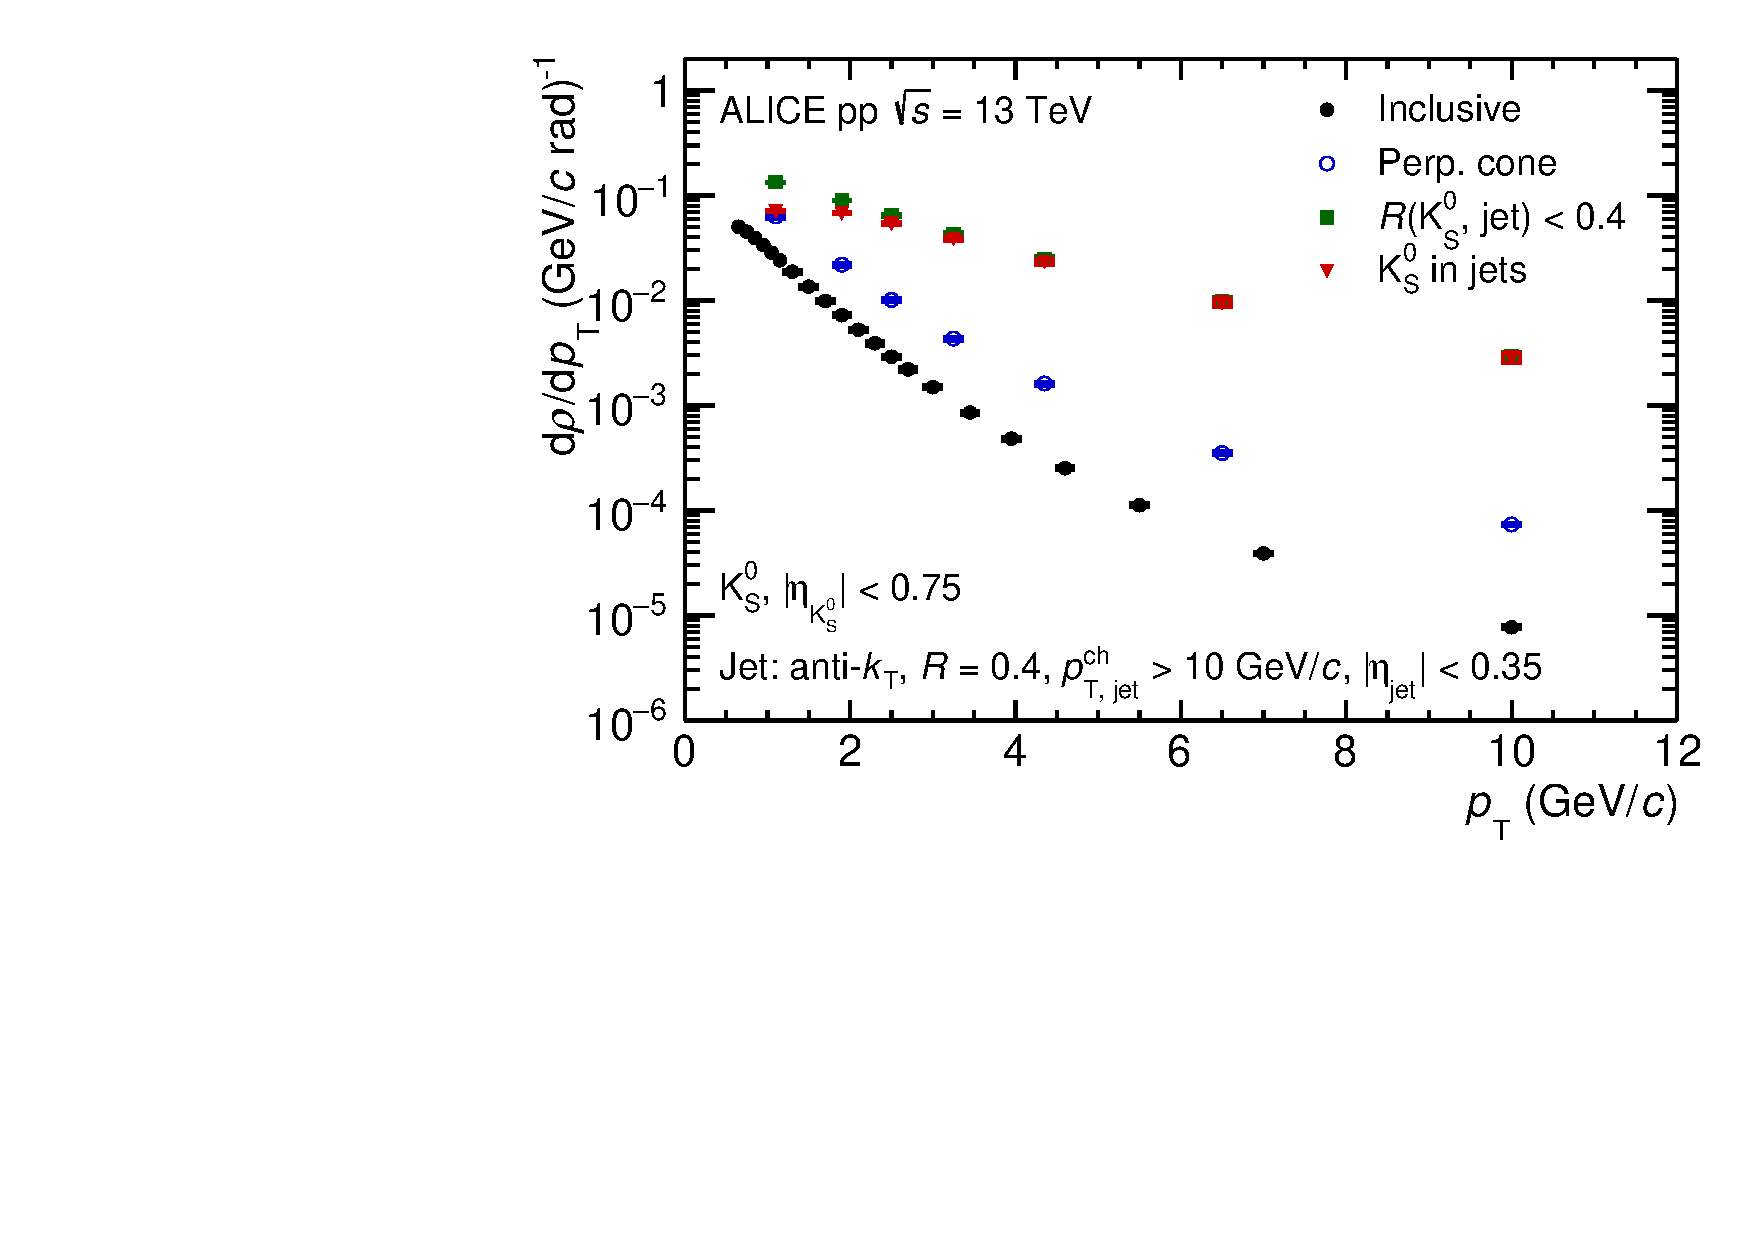
\includegraphics[width=.4\textwidth]{cf04_1}
		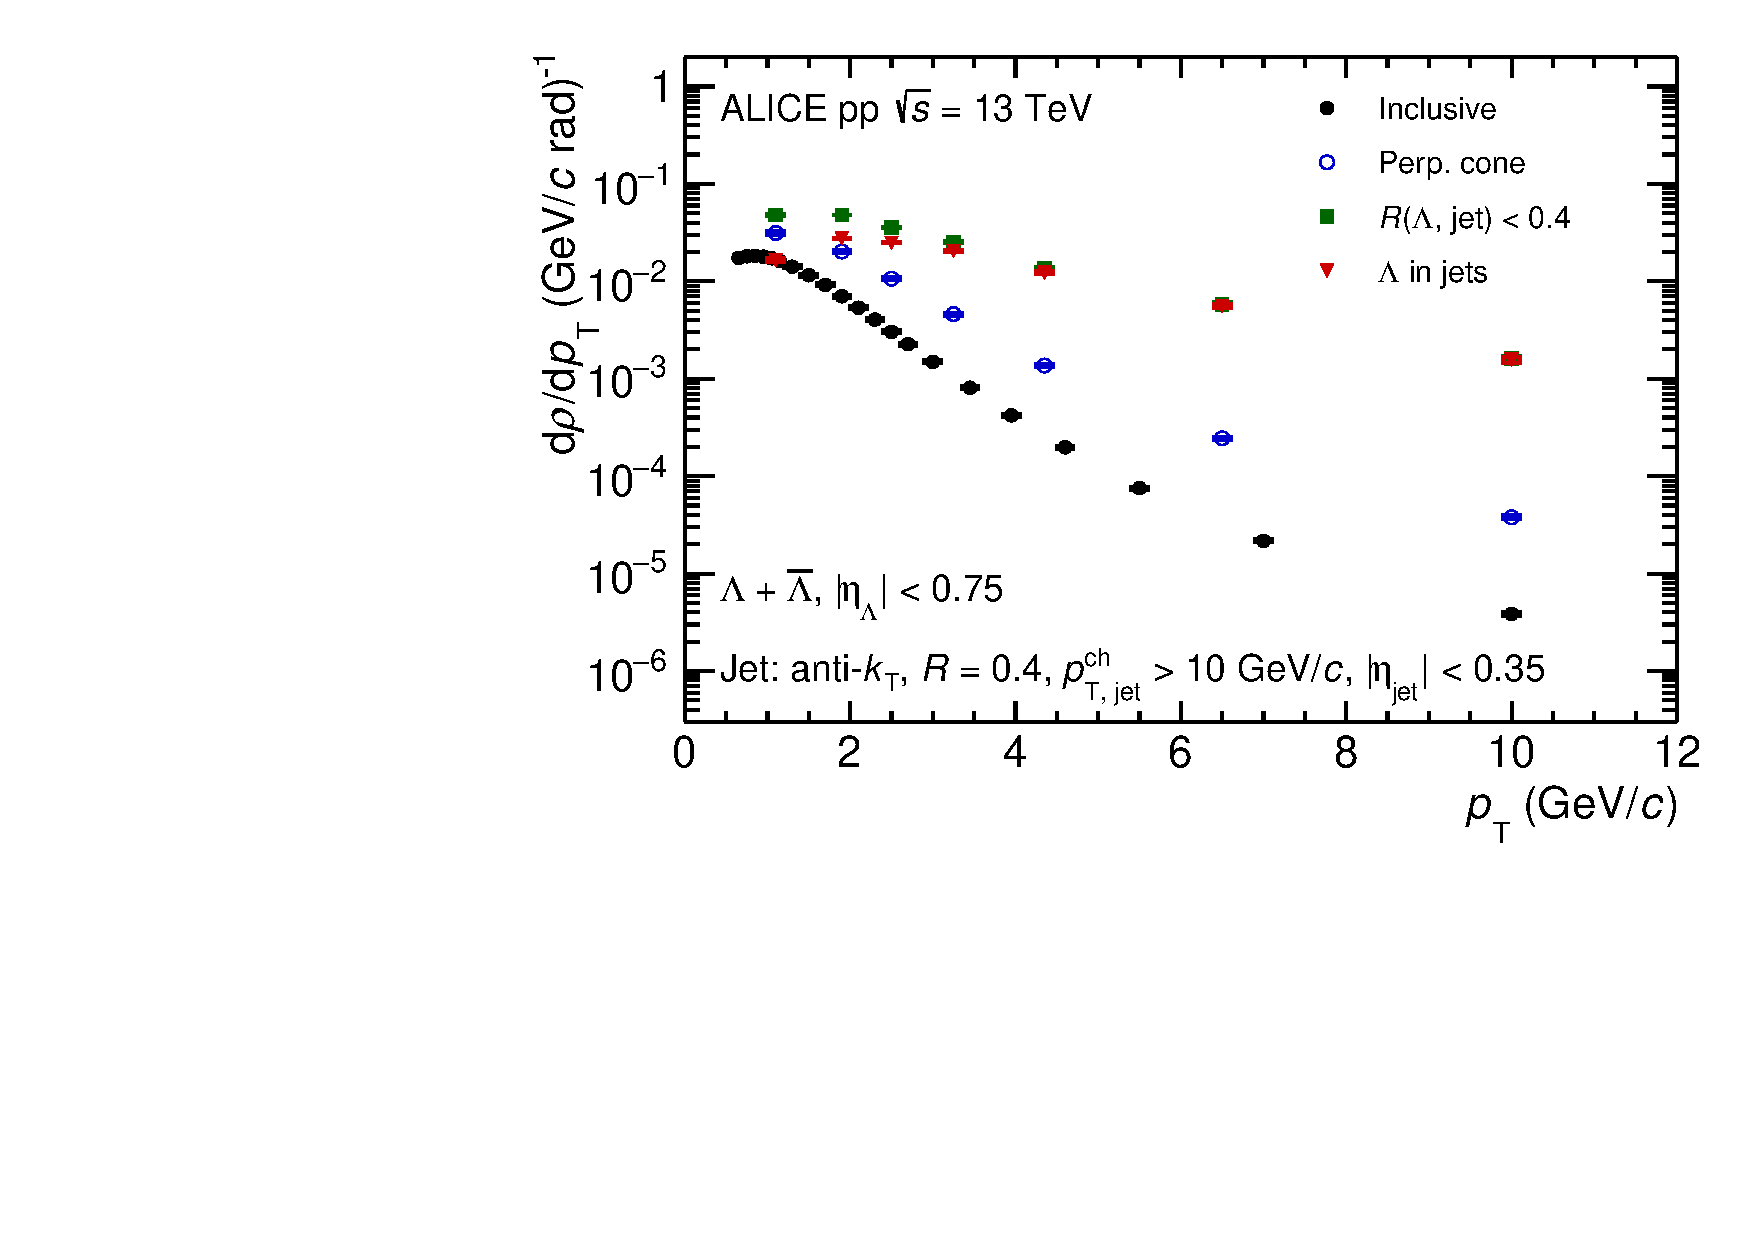
\includegraphics[width=.4\textwidth]{cf04_2}
		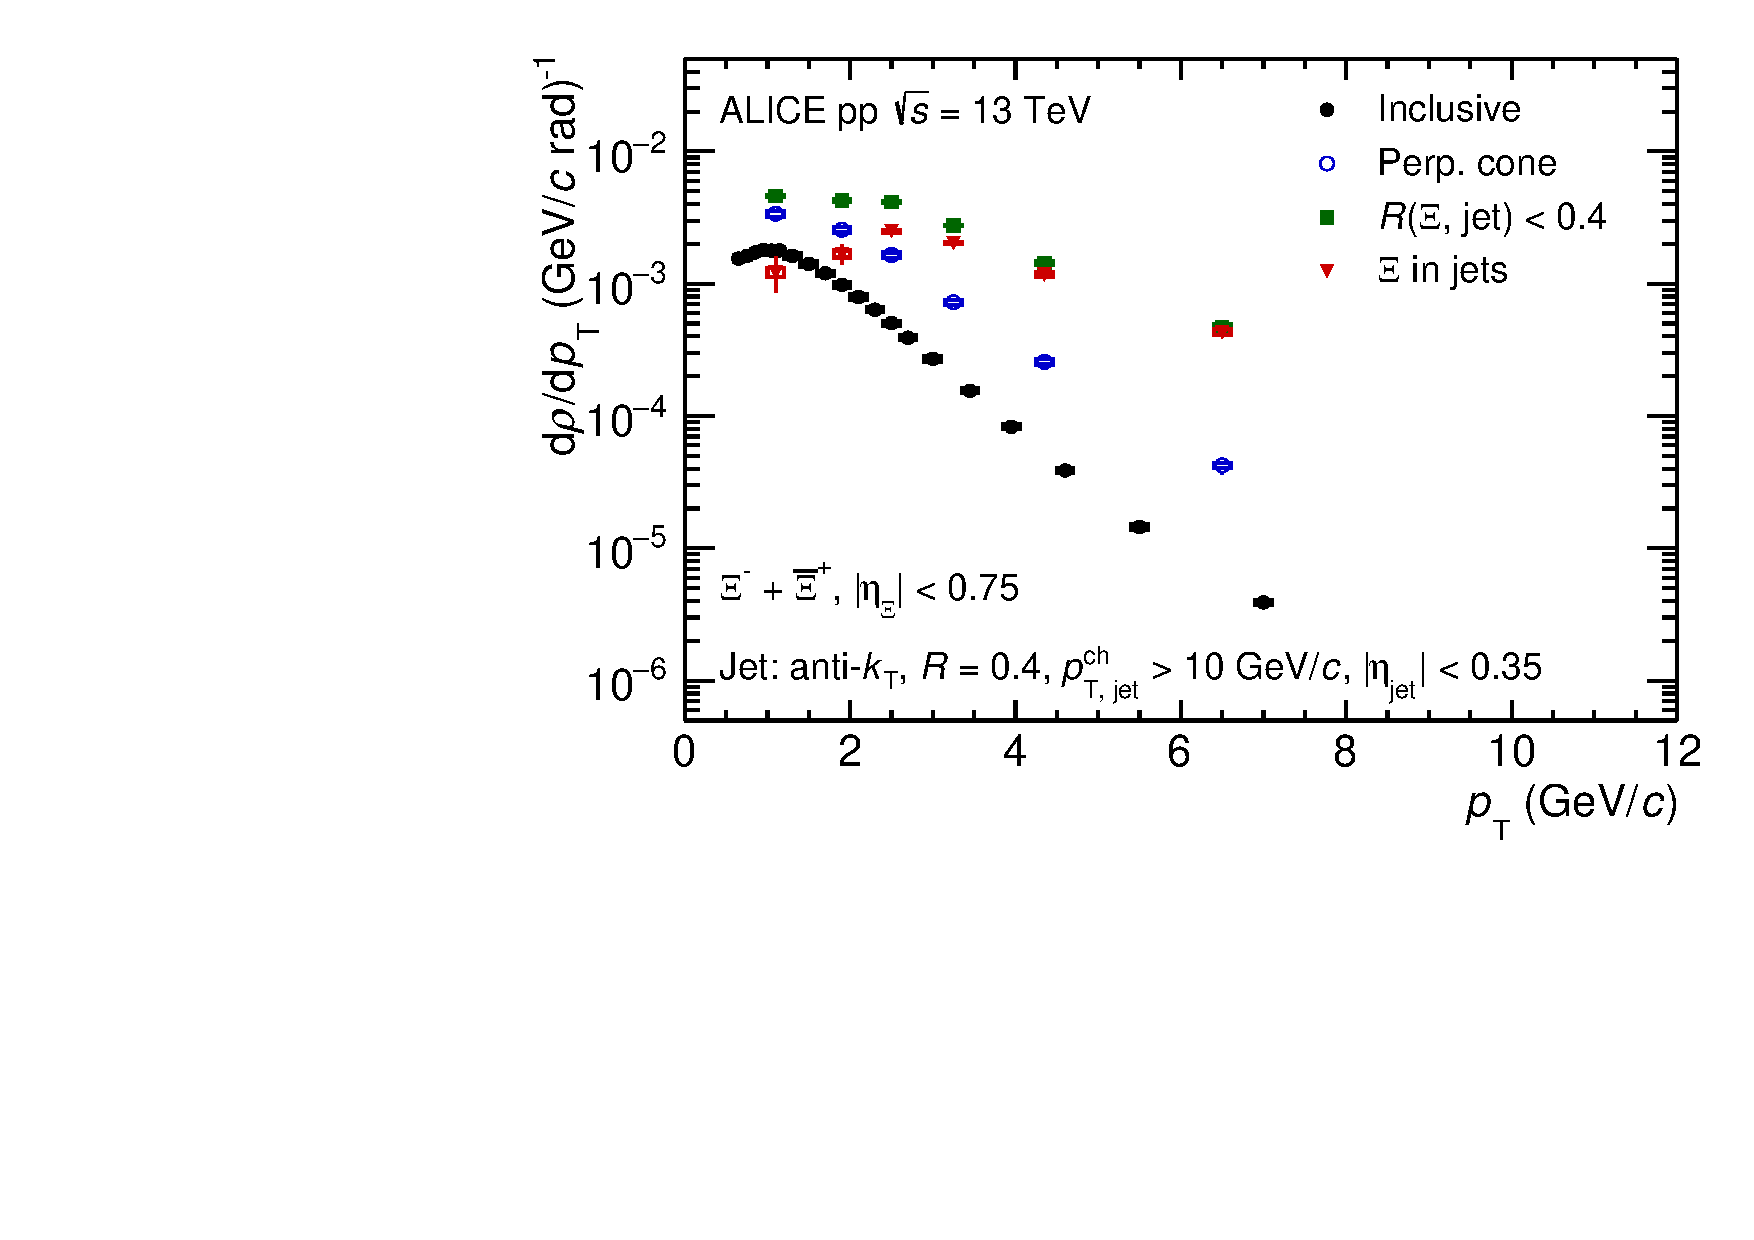
\includegraphics[width=.4\textwidth]{cf04_3}
		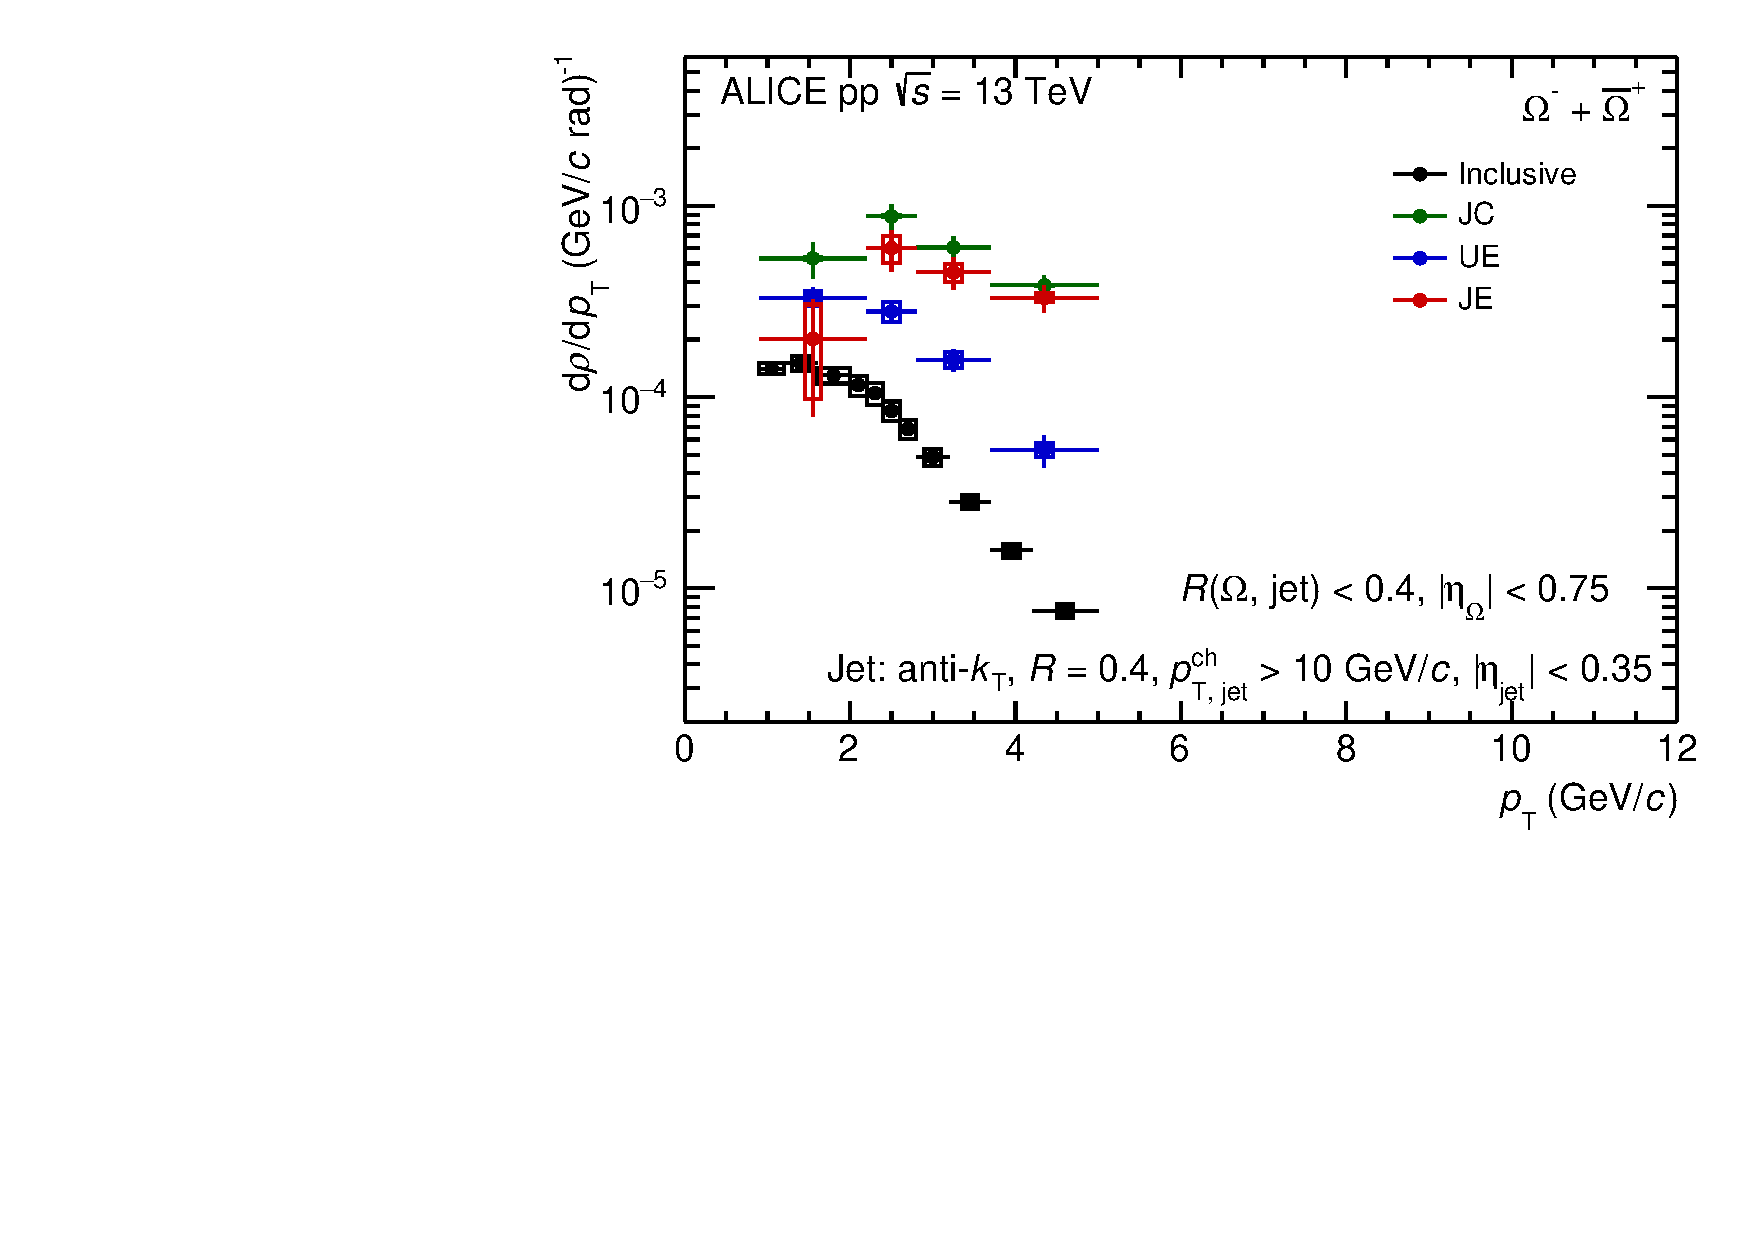
\includegraphics[width=.4\textwidth]{cf04_4}
	\end{center}
	\caption{$\pT$-differential density of $\kzero$, $\lmb + \almb$, $\X + \Ix$ and $\Om + \Mo$ in \pp at \thirteen. In those plots, the black point represent particles witch from minimum bias events, the green point represent particles which from the jet cones, the blue point represent particles within perpendicular cone of jet which associated with the underlying event and the red point represent the particle from the jet fragmentation.}
	\label{fig:ppSpect}
\end{figure}
\begin{figure}[!ht]
	\begin{center}
		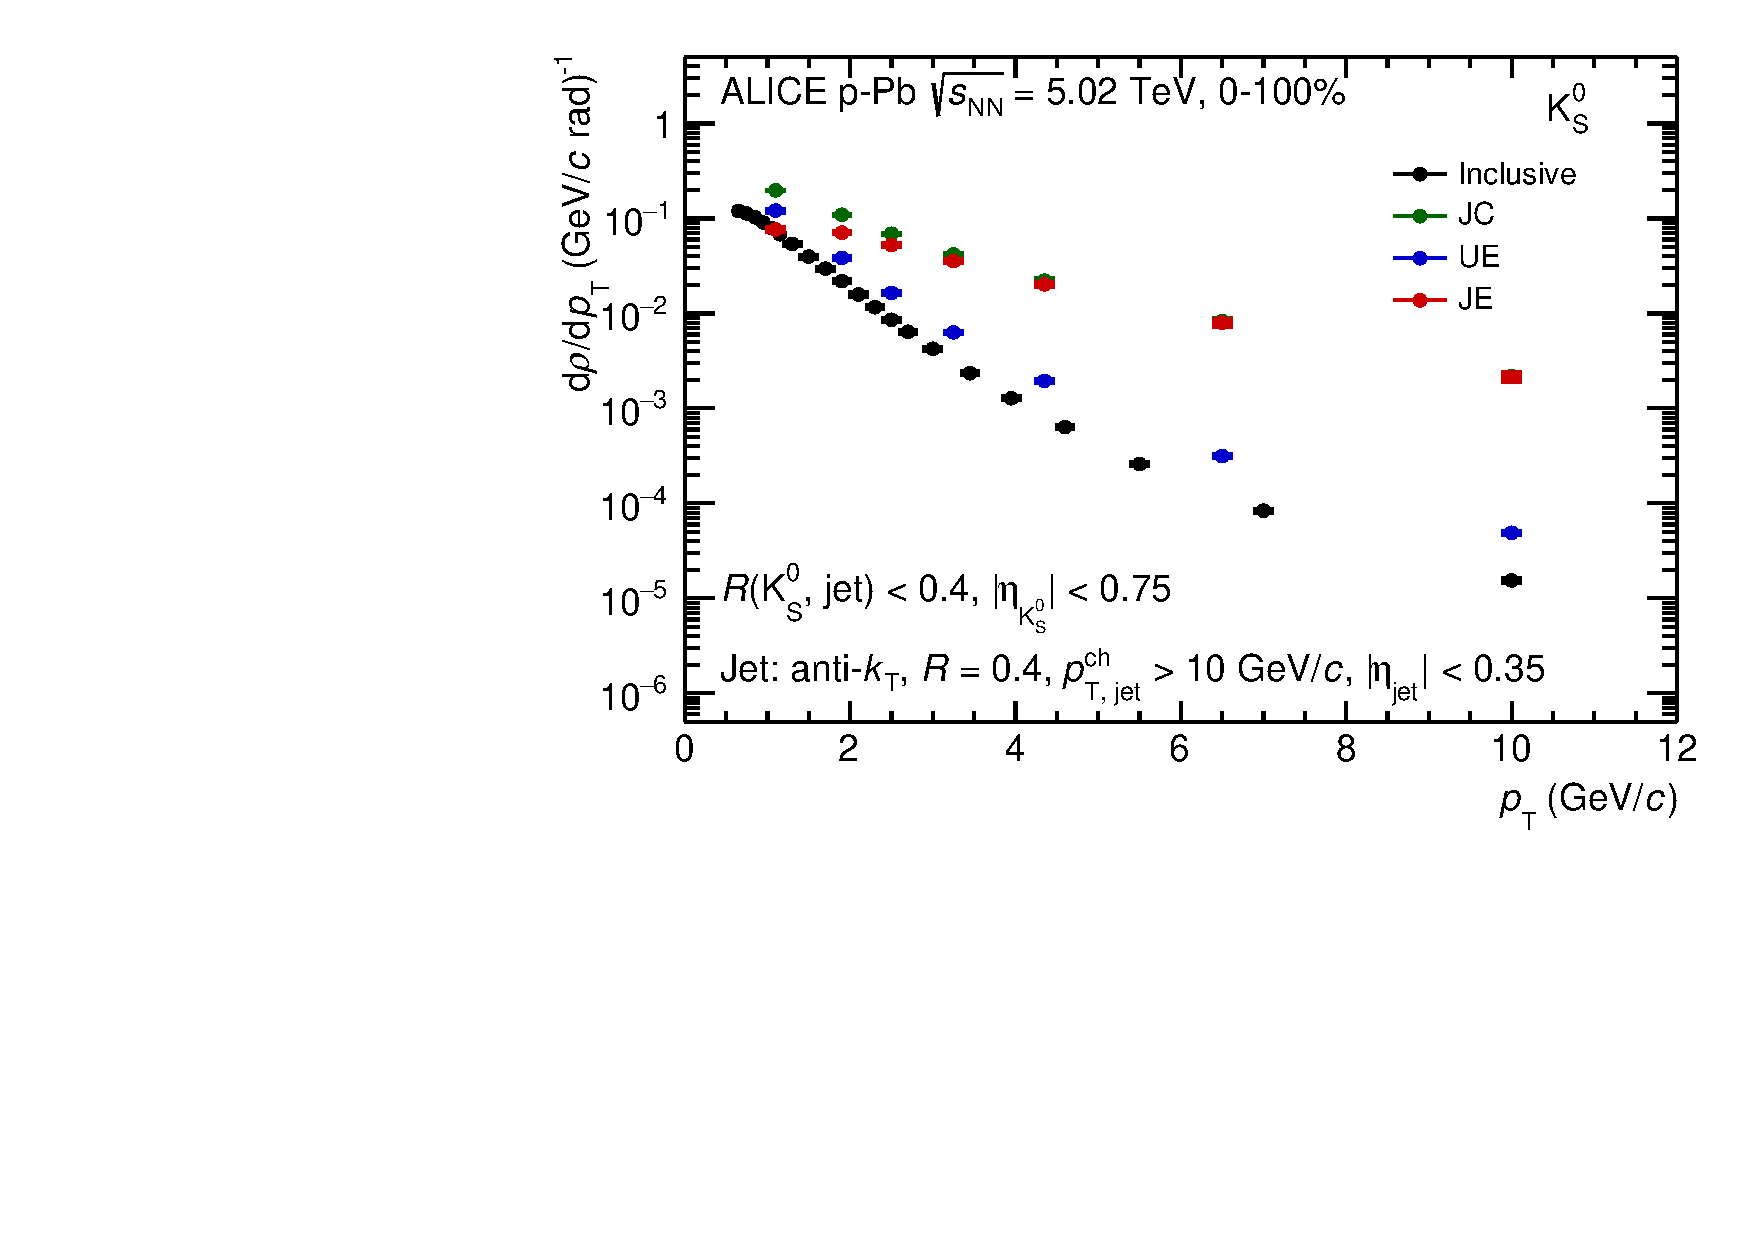
\includegraphics[width=.4\textwidth]{cf05_1}
		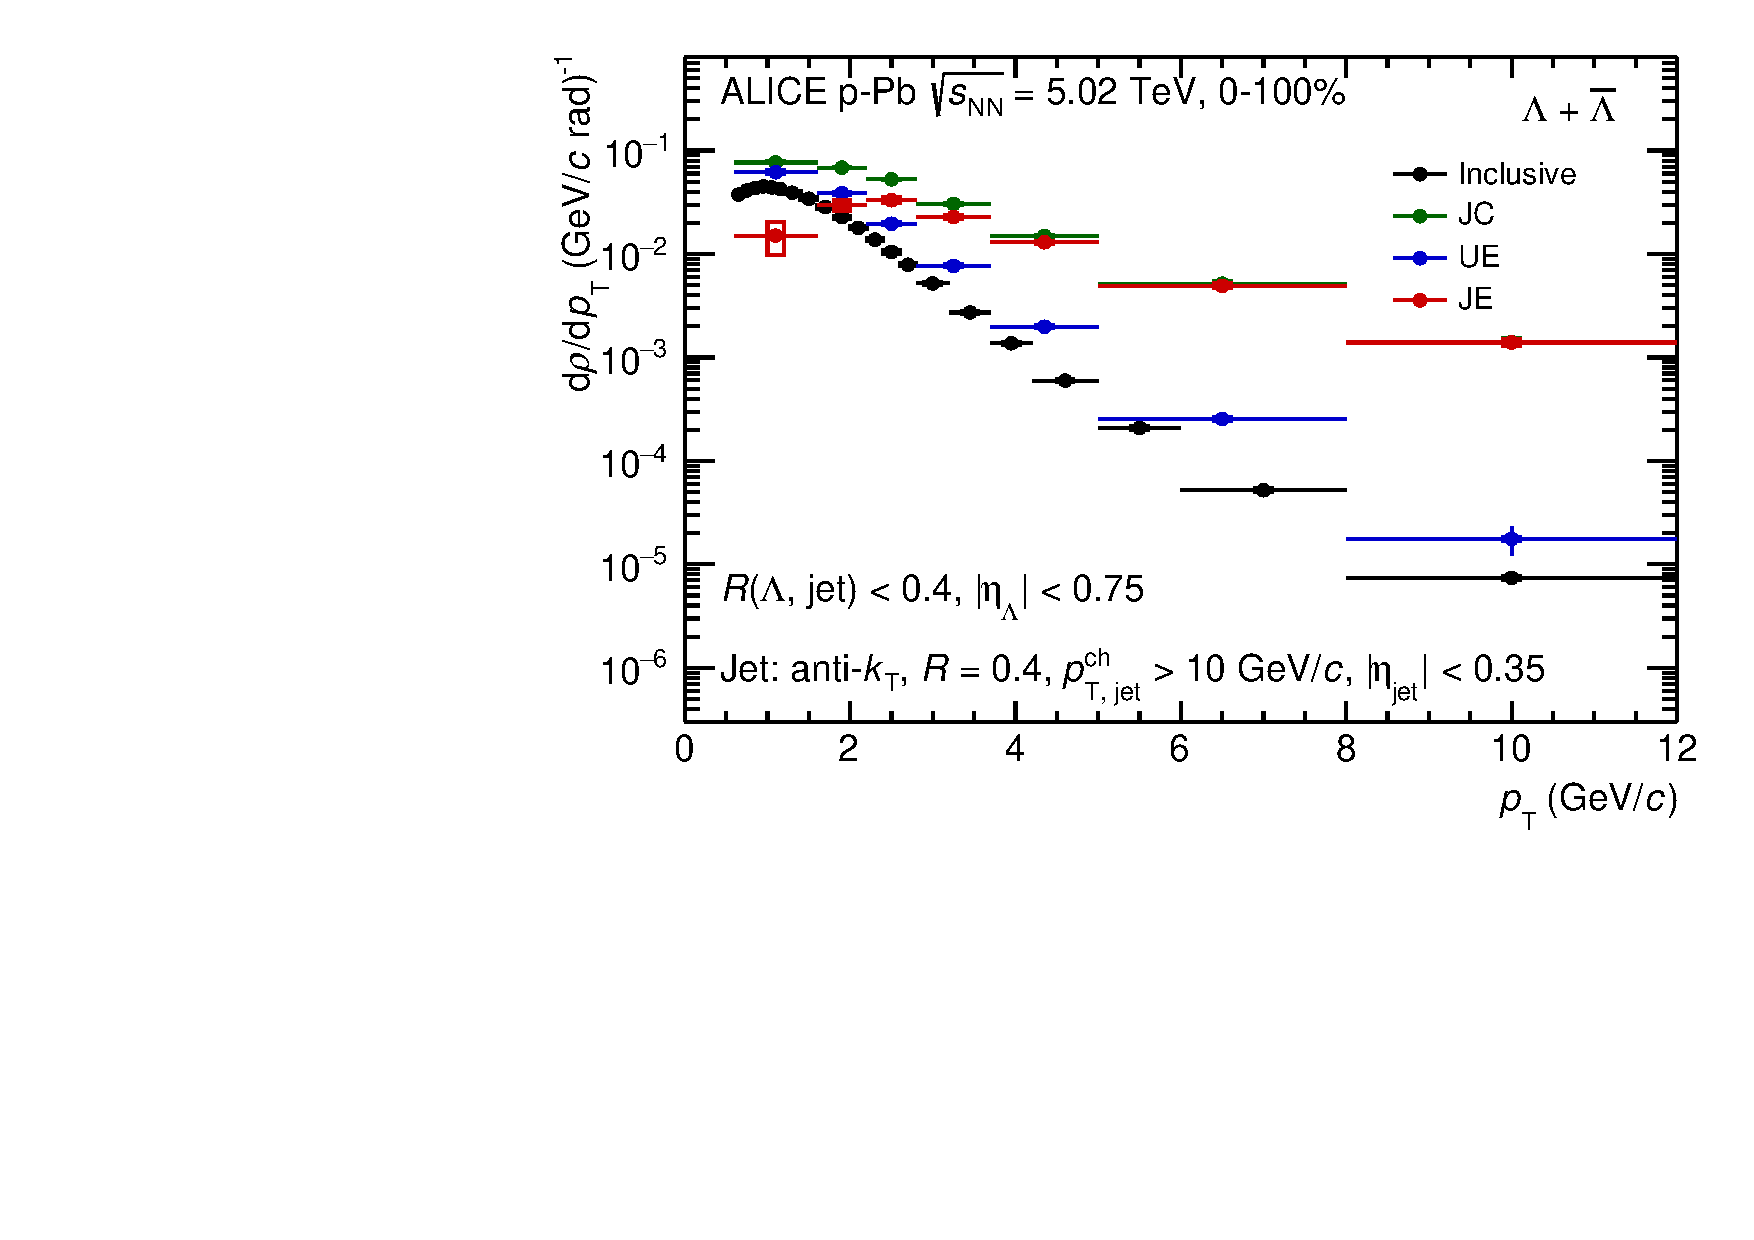
\includegraphics[width=.4\textwidth]{cf05_2}
		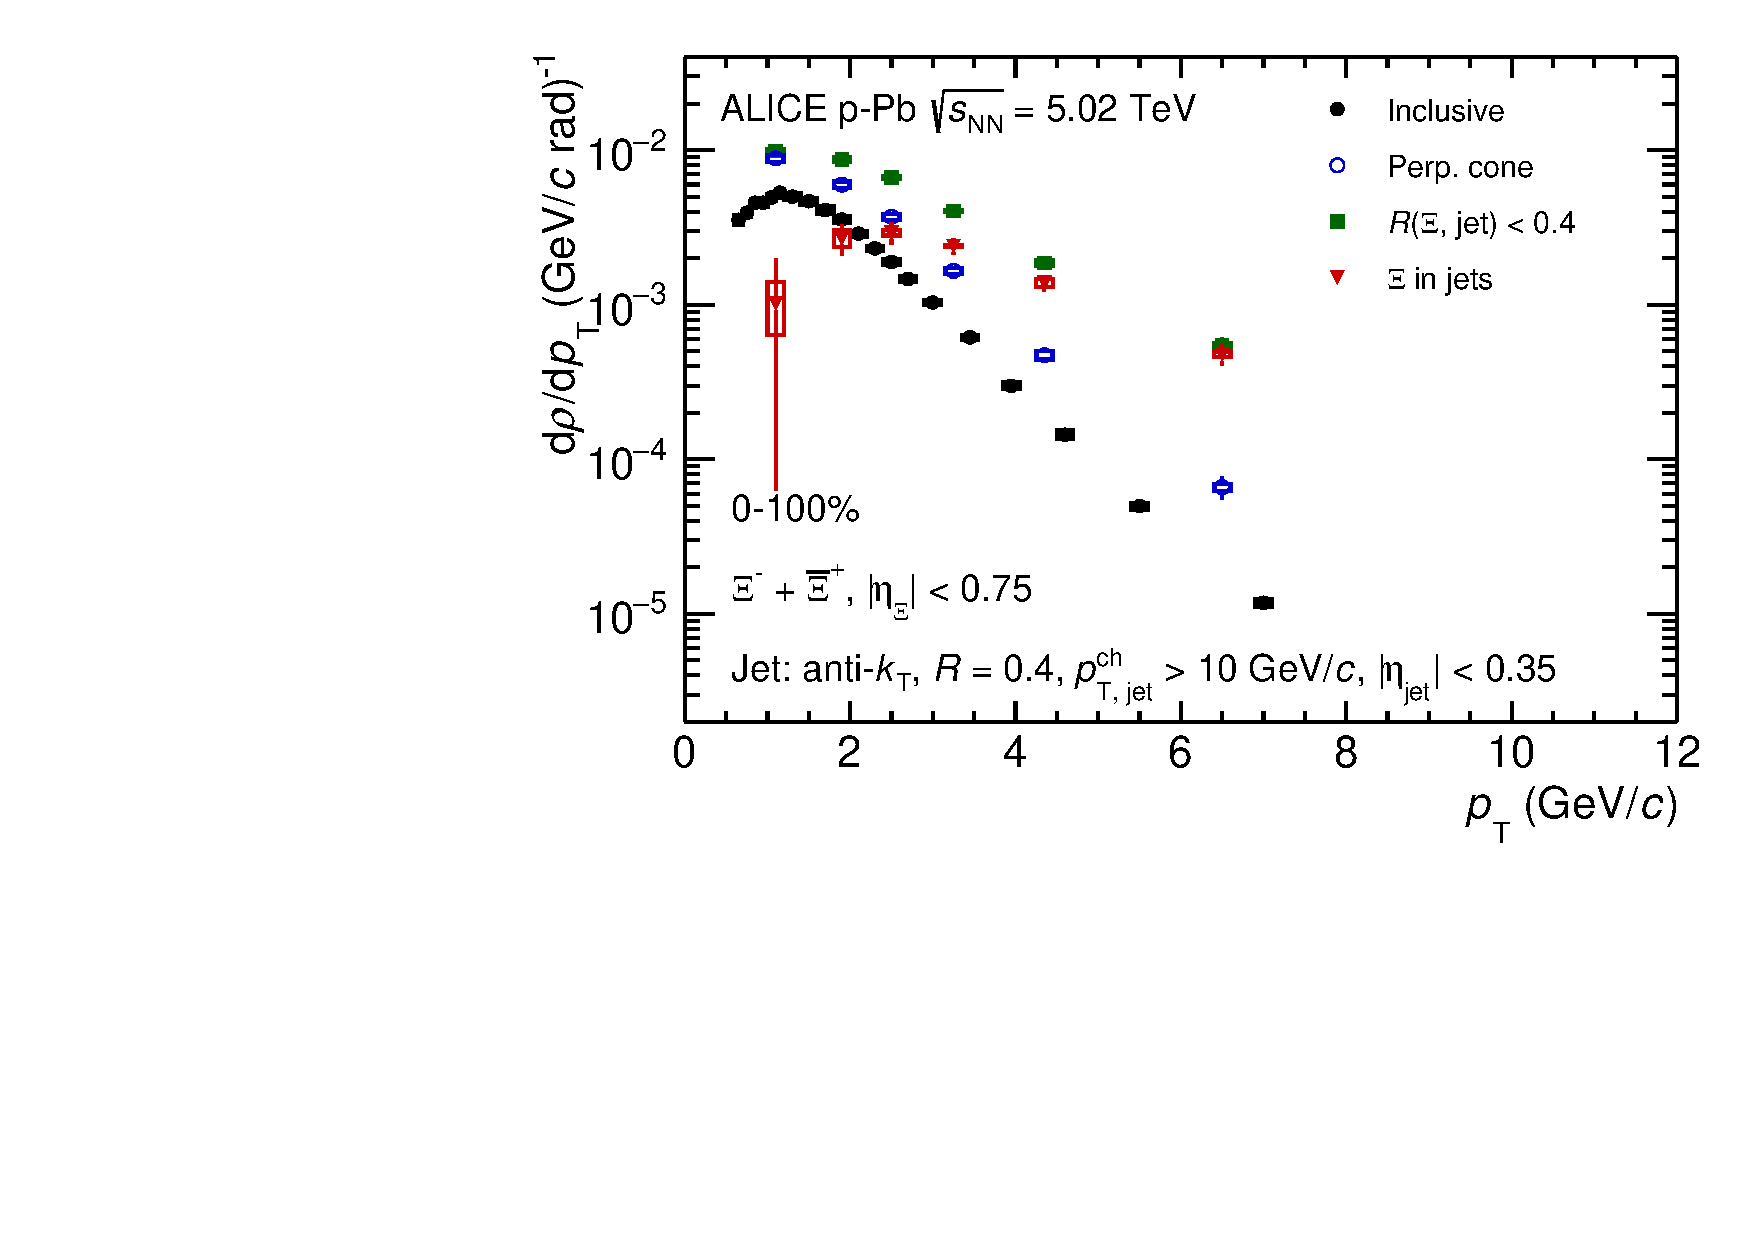
\includegraphics[width=.4\textwidth]{cf05_3}
		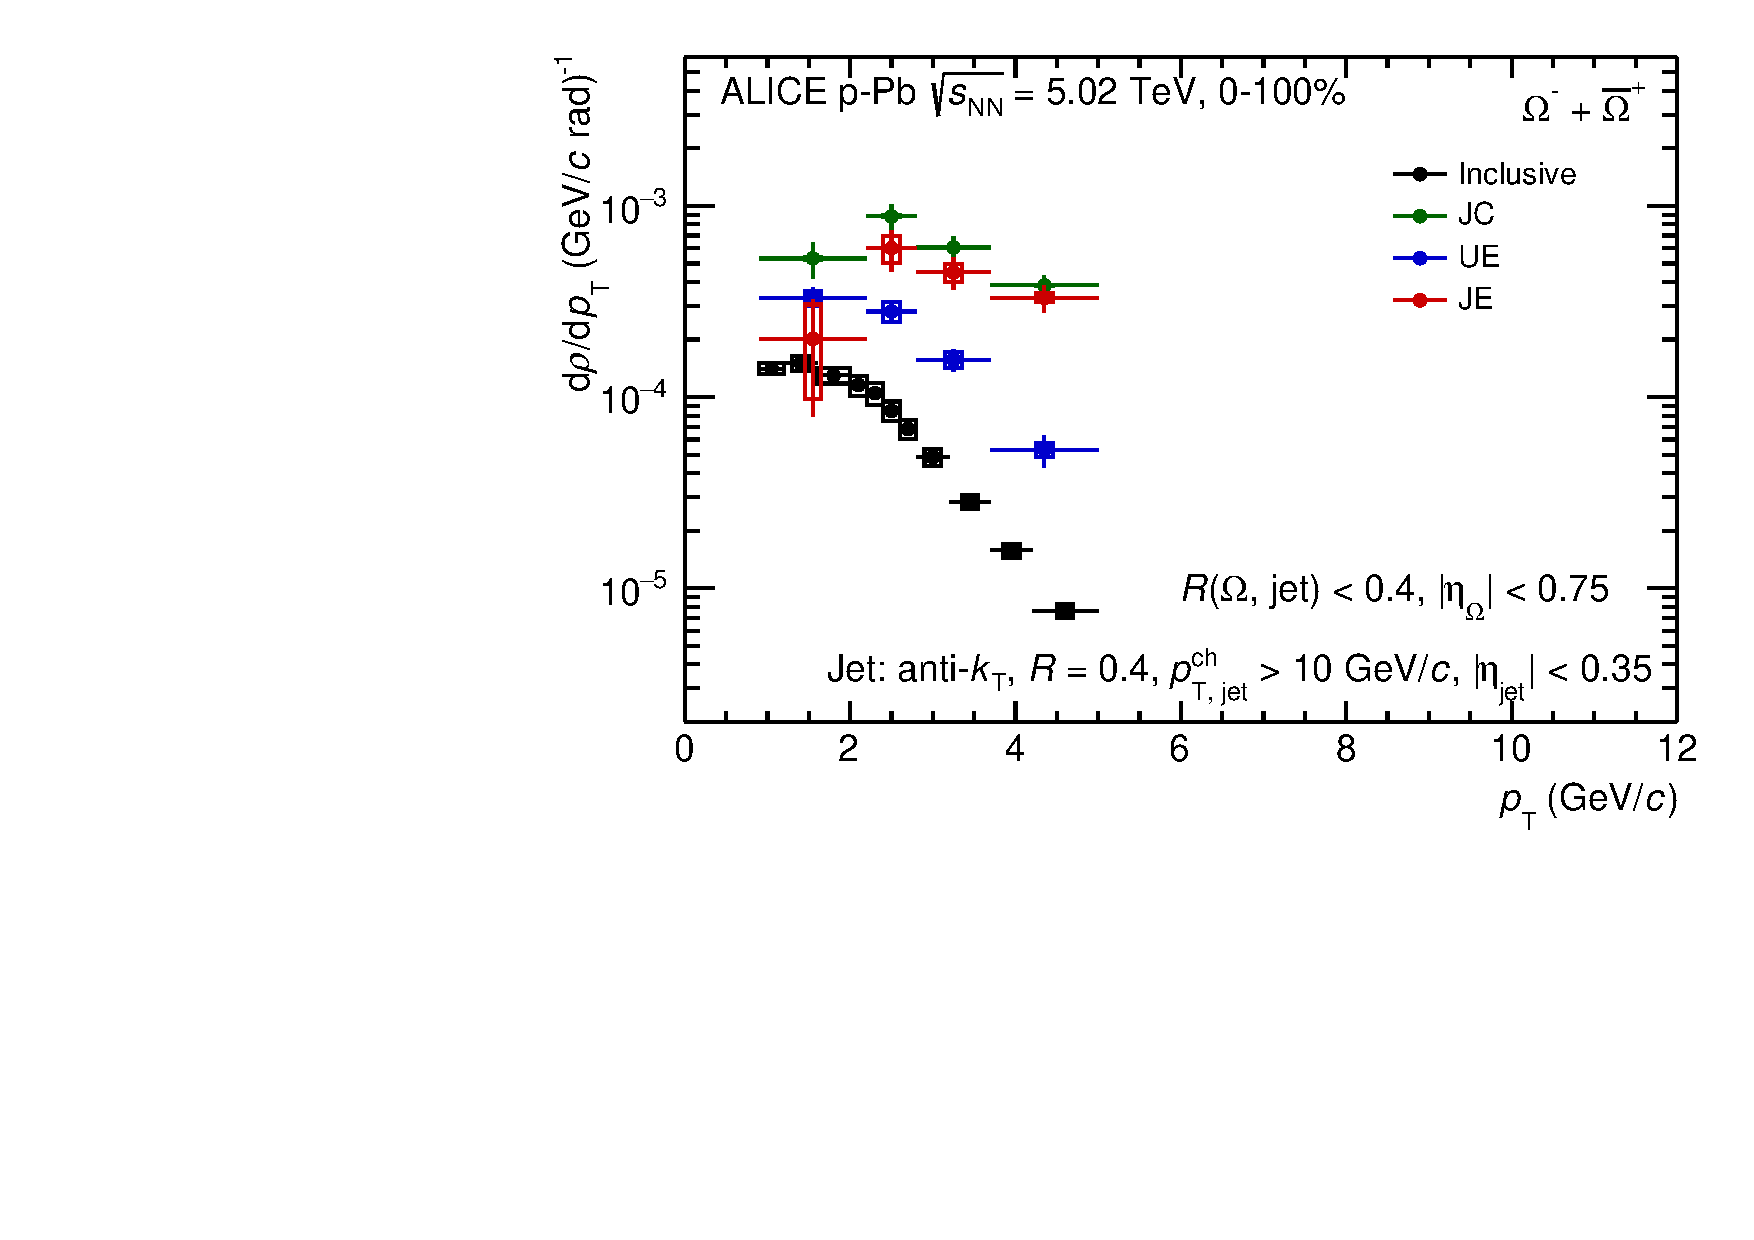
\includegraphics[width=.4\textwidth]{cf05_4}
	\end{center}
	\caption{$\pT$-differential density of $\kzero$, $\lmb + \almb$, $\X + \Ix$ and $\Om + \Mo$ in 0-100\% in \pPb at \fivenn. In those plots, the black point depicts particles witch from minimum bias events, the green point depicts particles which from the jet cones, the blue point depicts particles within perpendicular cone of jet which associated with the underlying event and the red point depicts the particle from the jet fragmentation.}
	\label{fig:pPbSpect}
\end{figure}

The $\pT$ distributions of $\kzero$, $\lmb + \almb$ and $\X + \Ix$ for the event classes defined in Tab.~\ref{tab:multi} are show in Fig.~\ref{fig:pPbSpectwCent}. The inclusive distributions become harder with increasing charged-particle multiplicity. Particles in JE, which generated by jet fragmentation, are systematically independent with centrality classes.
\begin{figure}[!ht]
	\begin{center}
		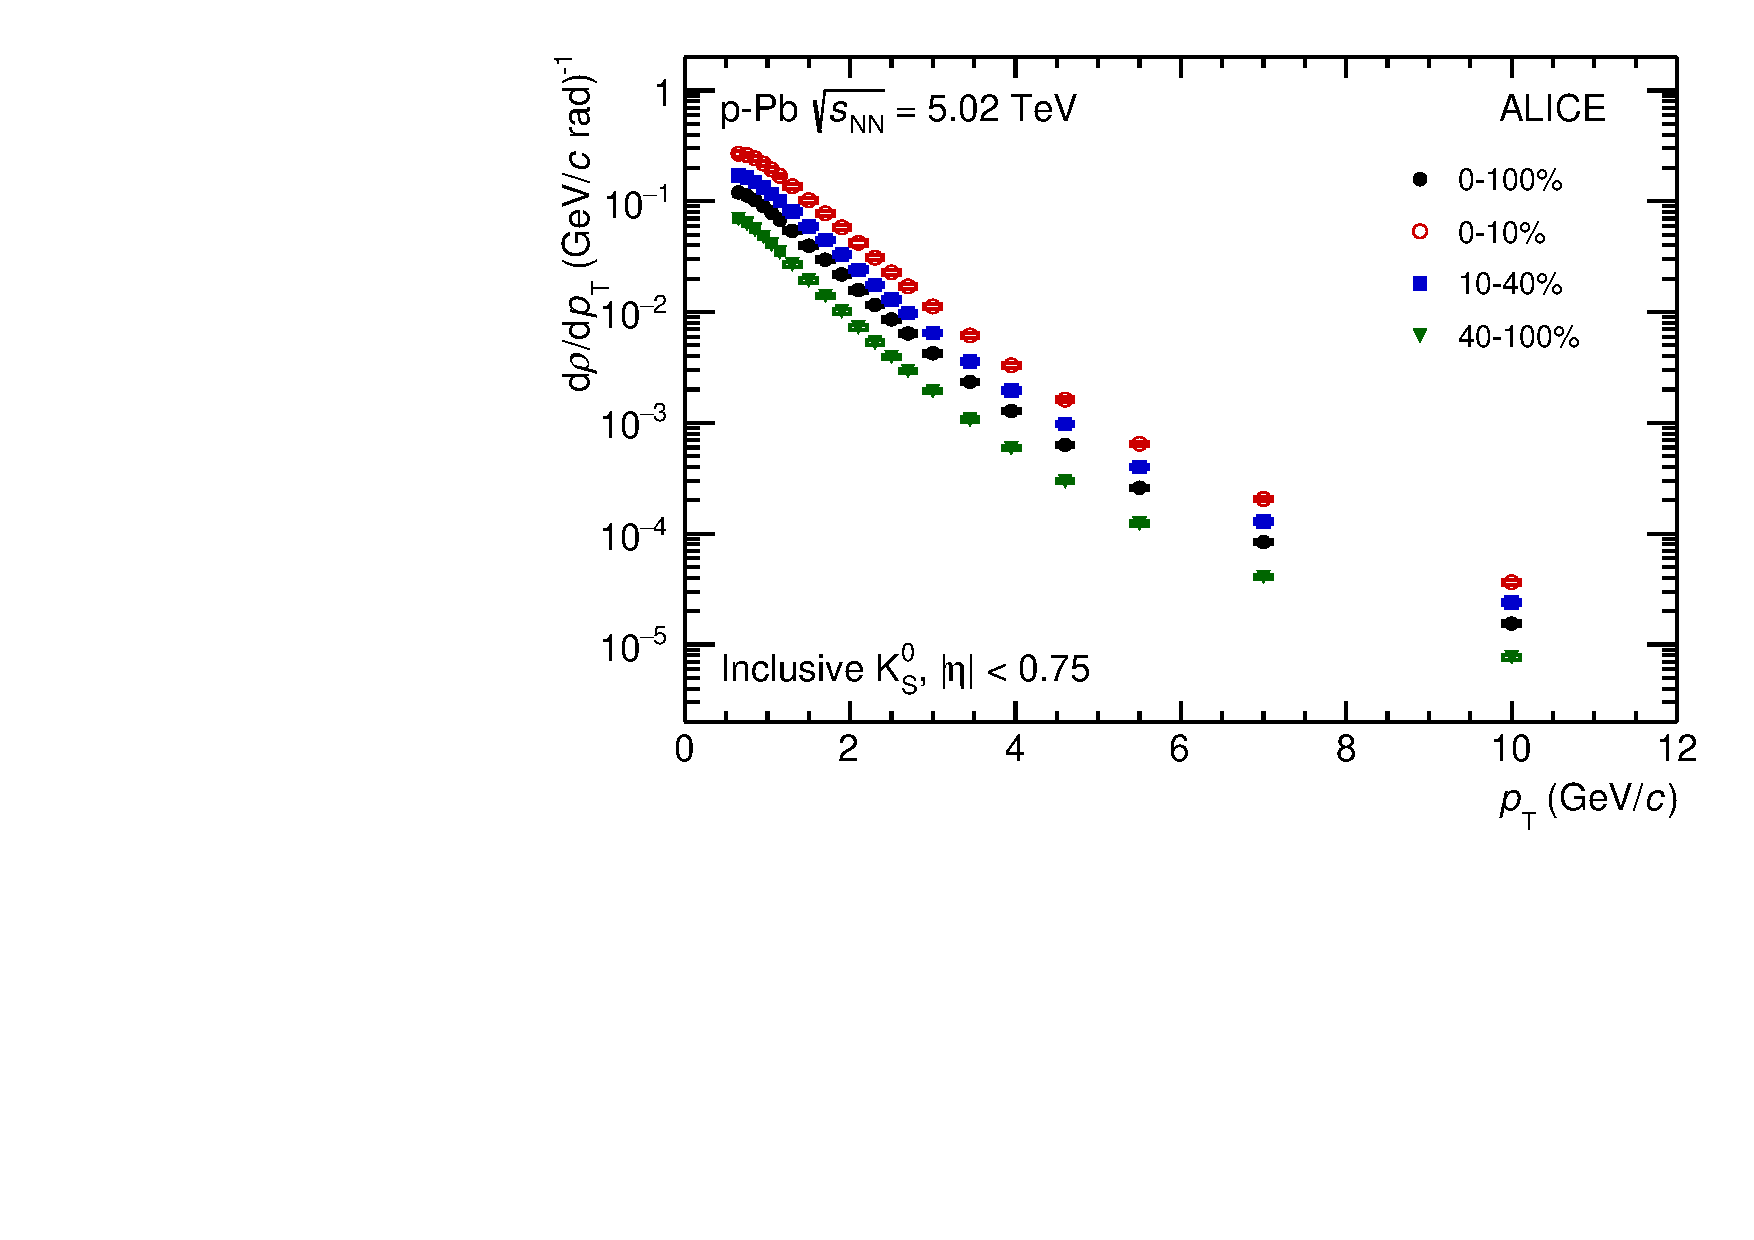
\includegraphics[width=.3\textwidth]{cf06_1}
		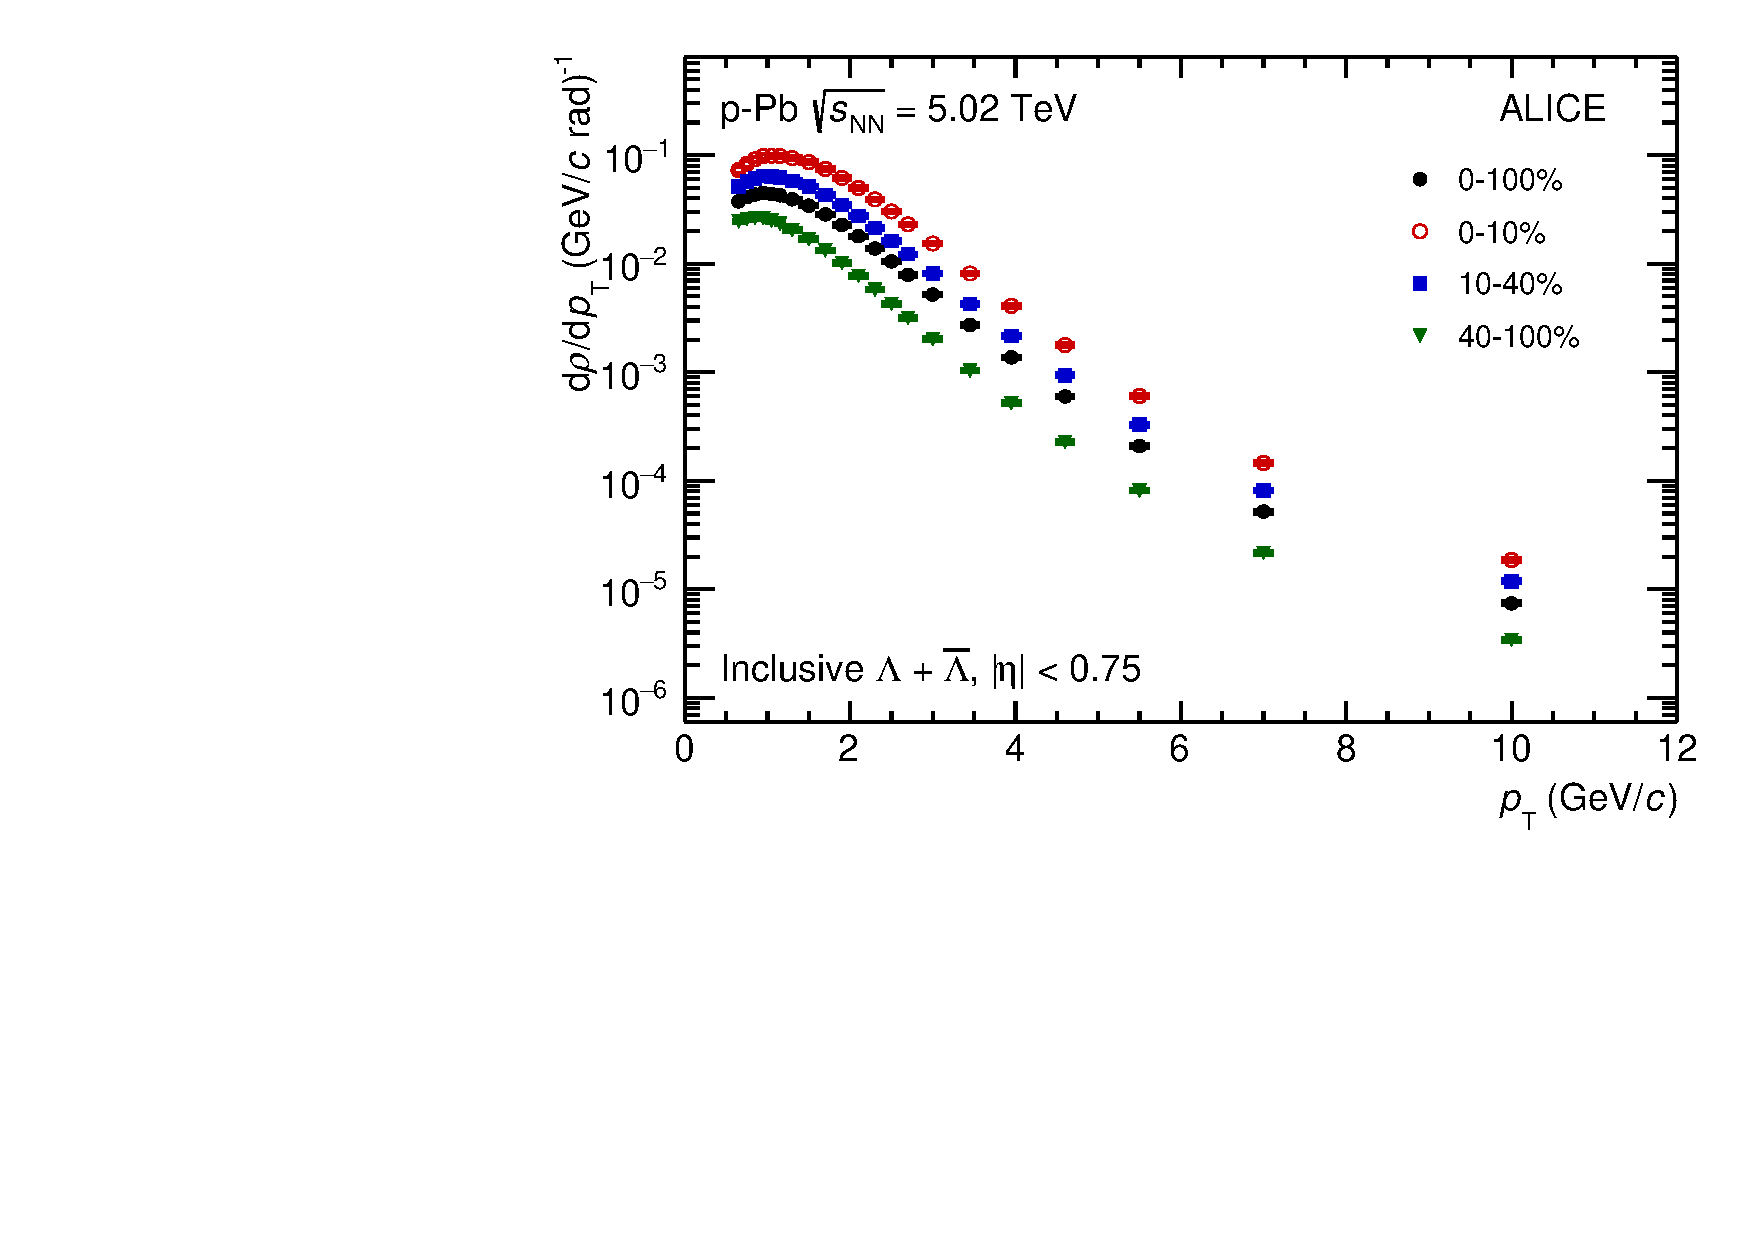
\includegraphics[width=.3\textwidth]{cf06_2}
		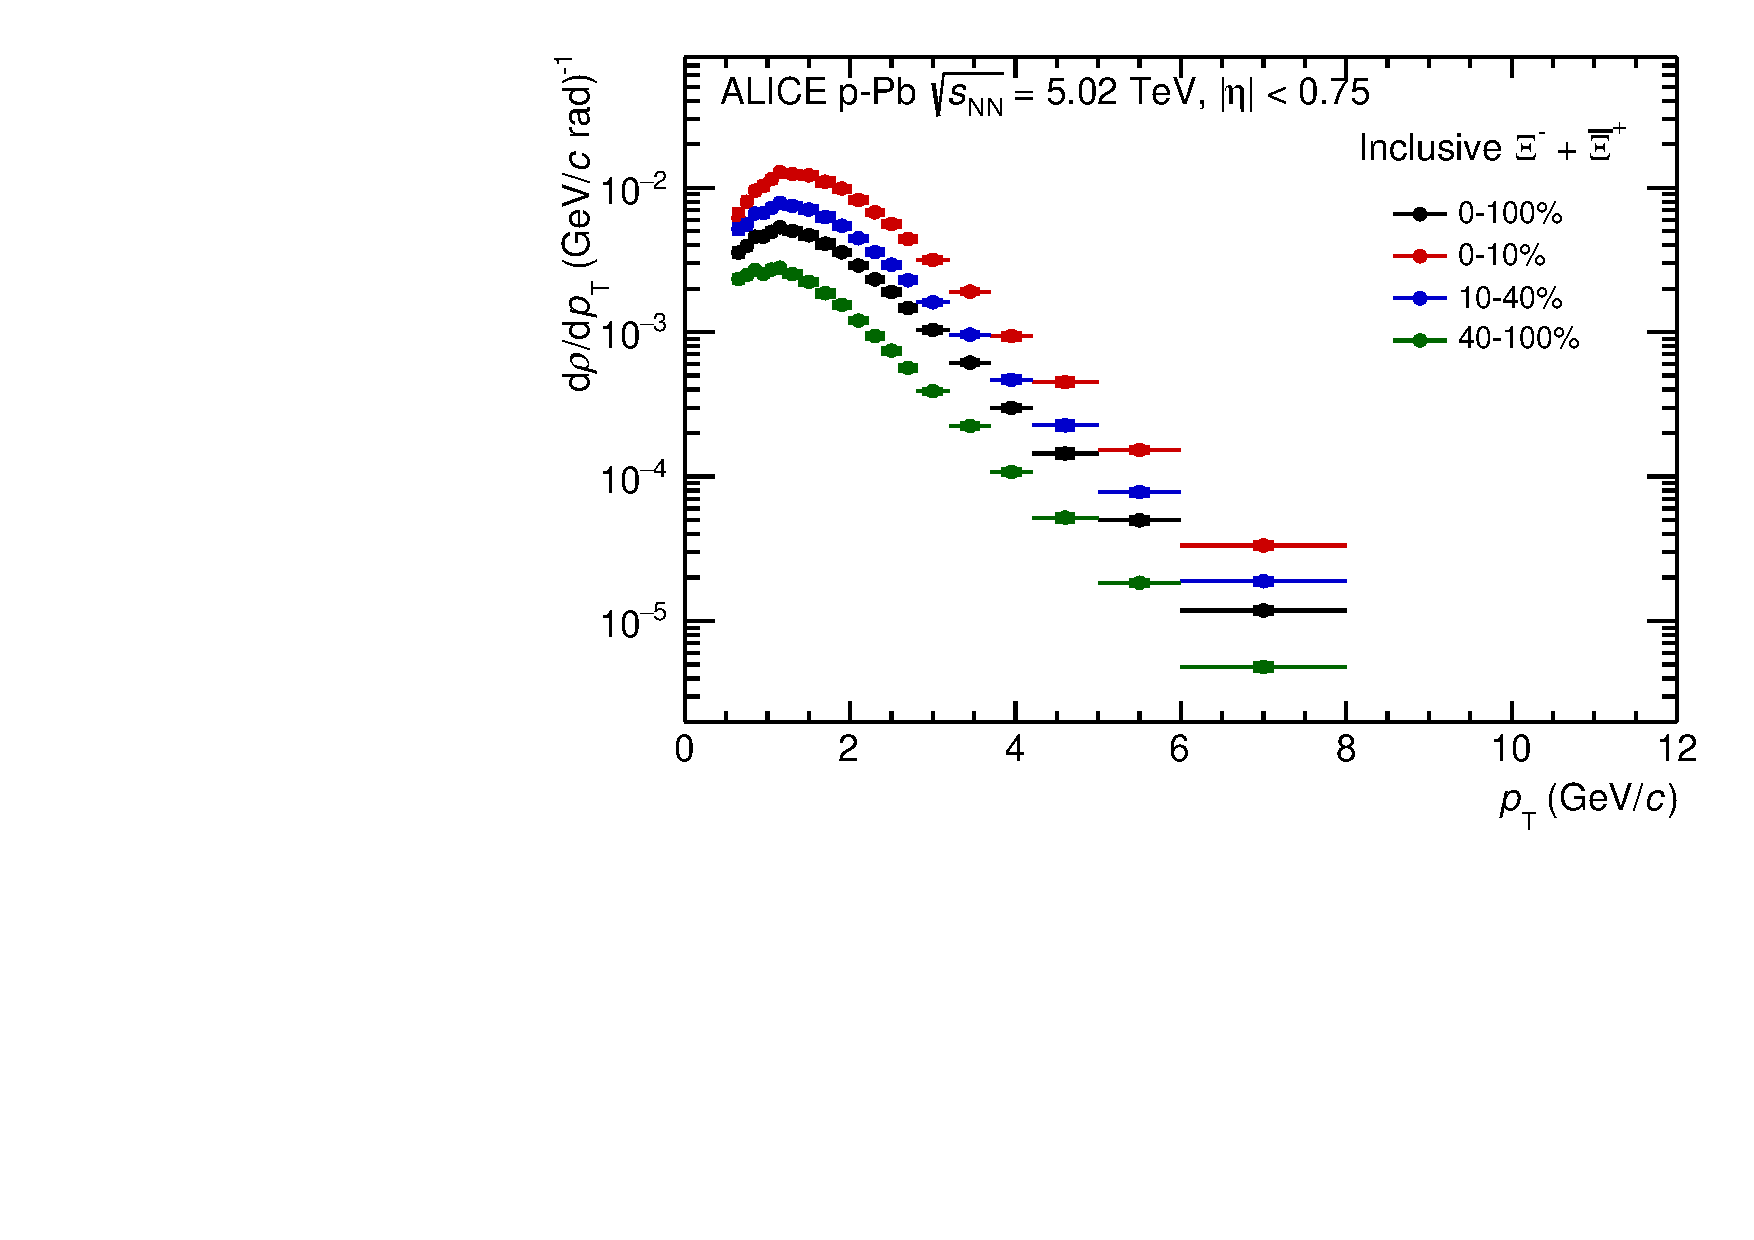
\includegraphics[width=.3\textwidth]{cf06_3}
		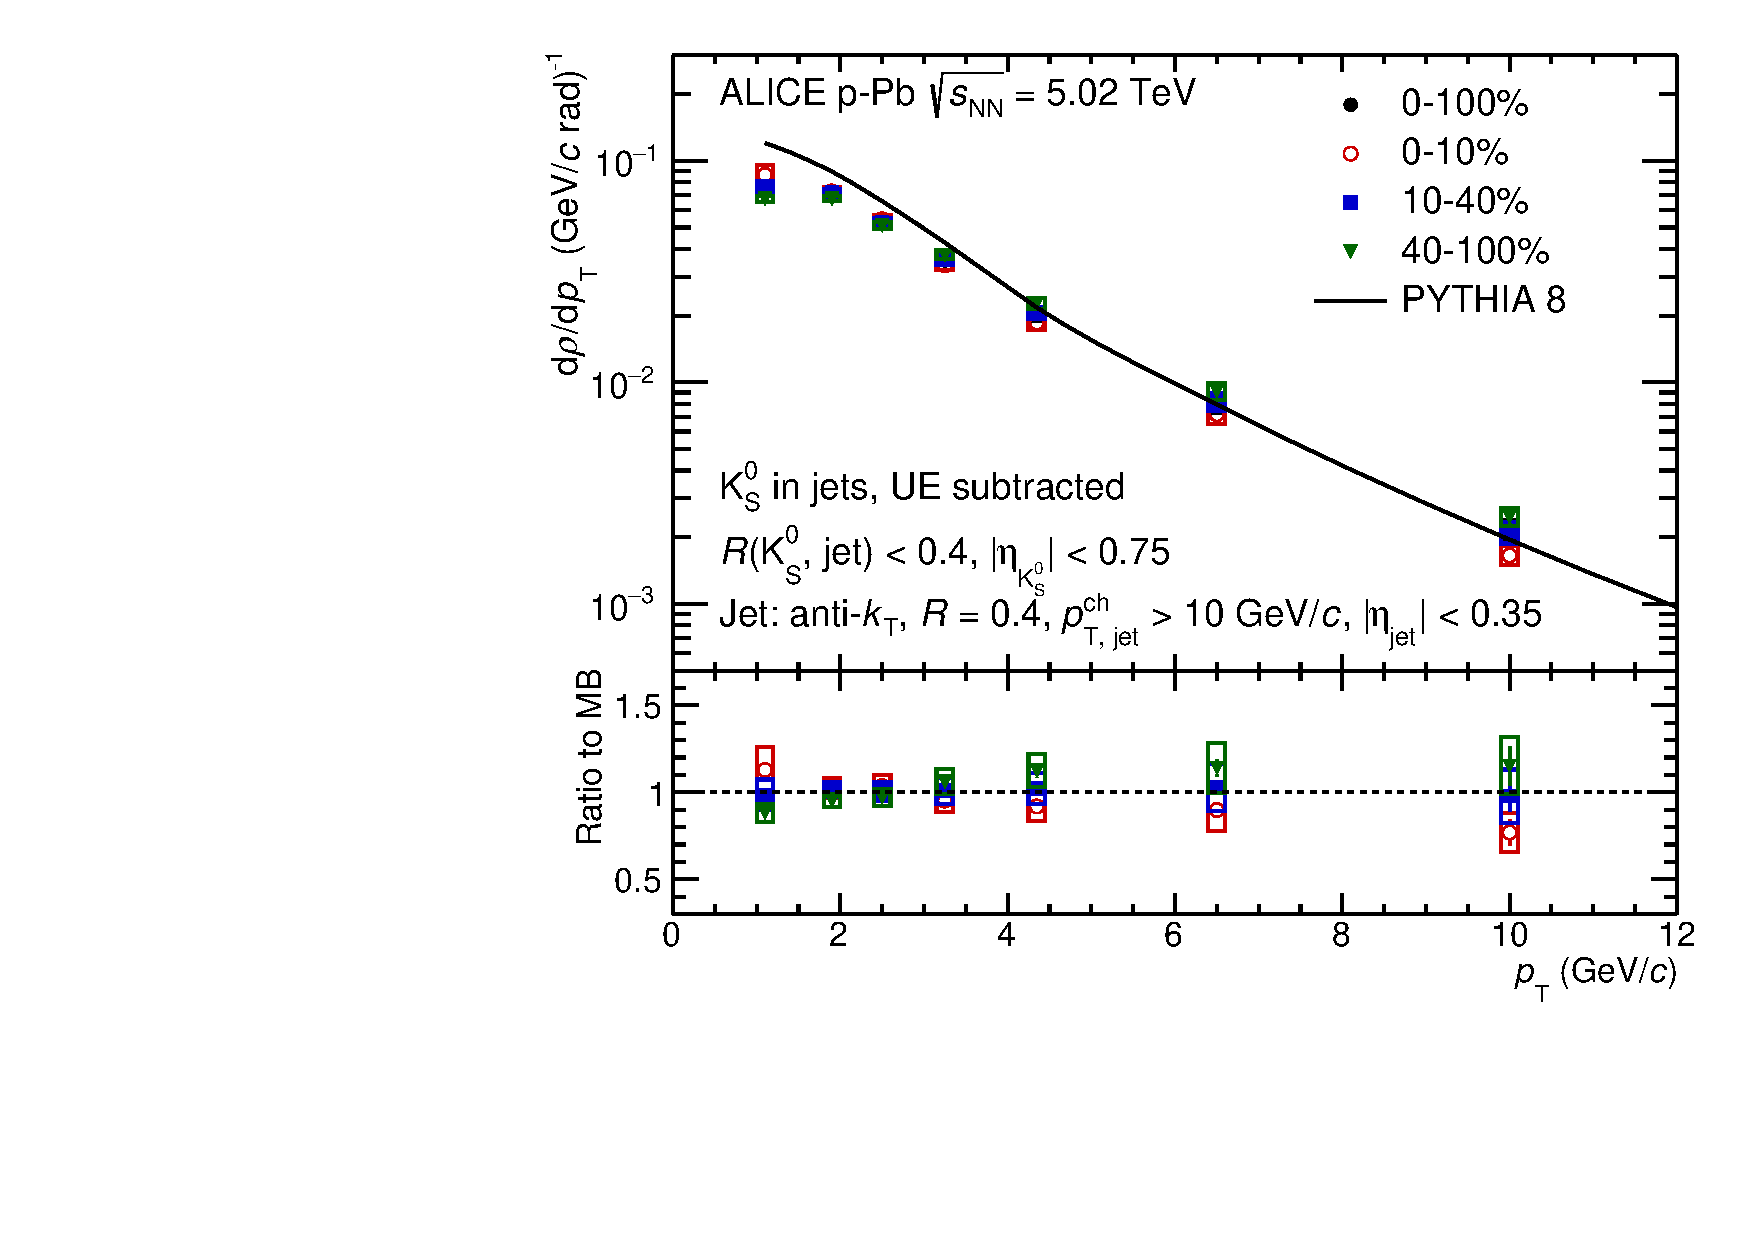
\includegraphics[width=.3\textwidth]{cf06_4}
		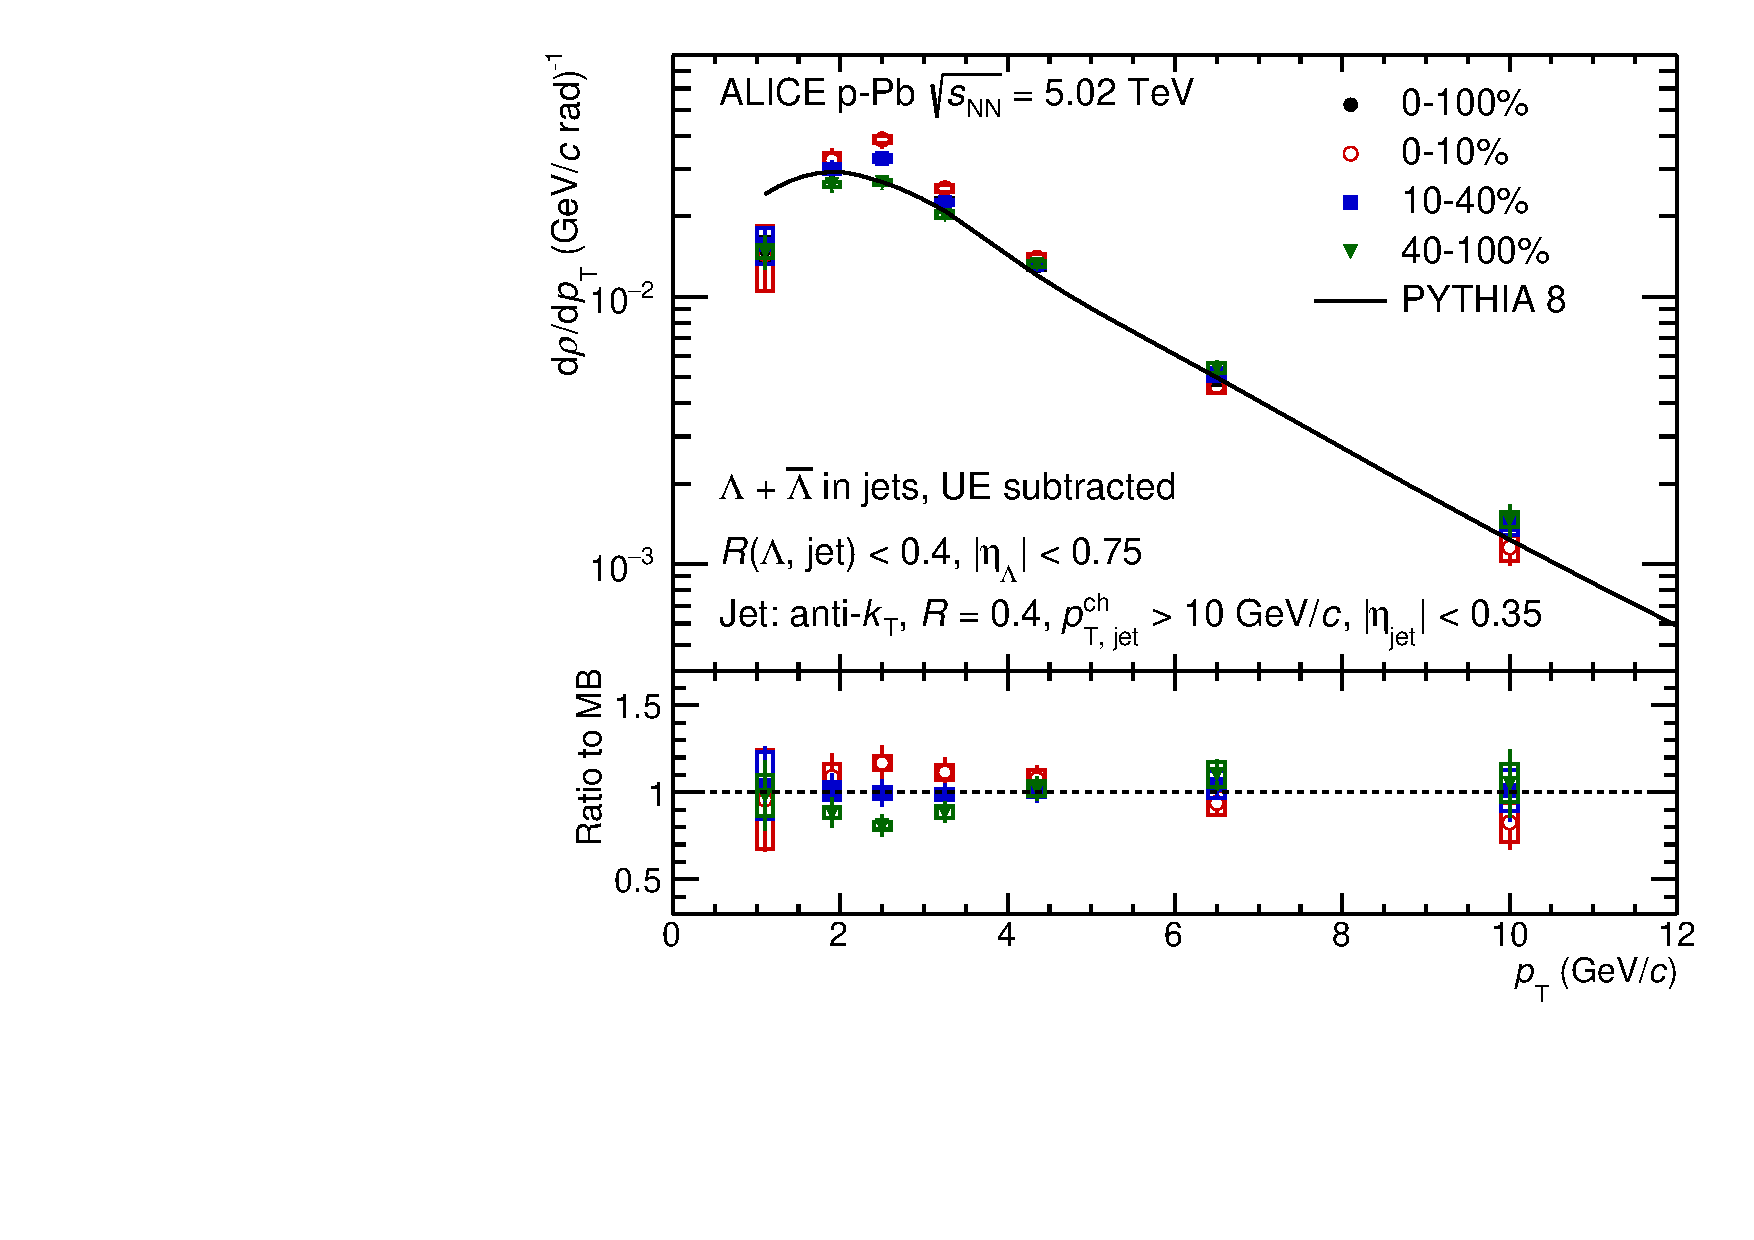
\includegraphics[width=.3\textwidth]{cf06_5}
		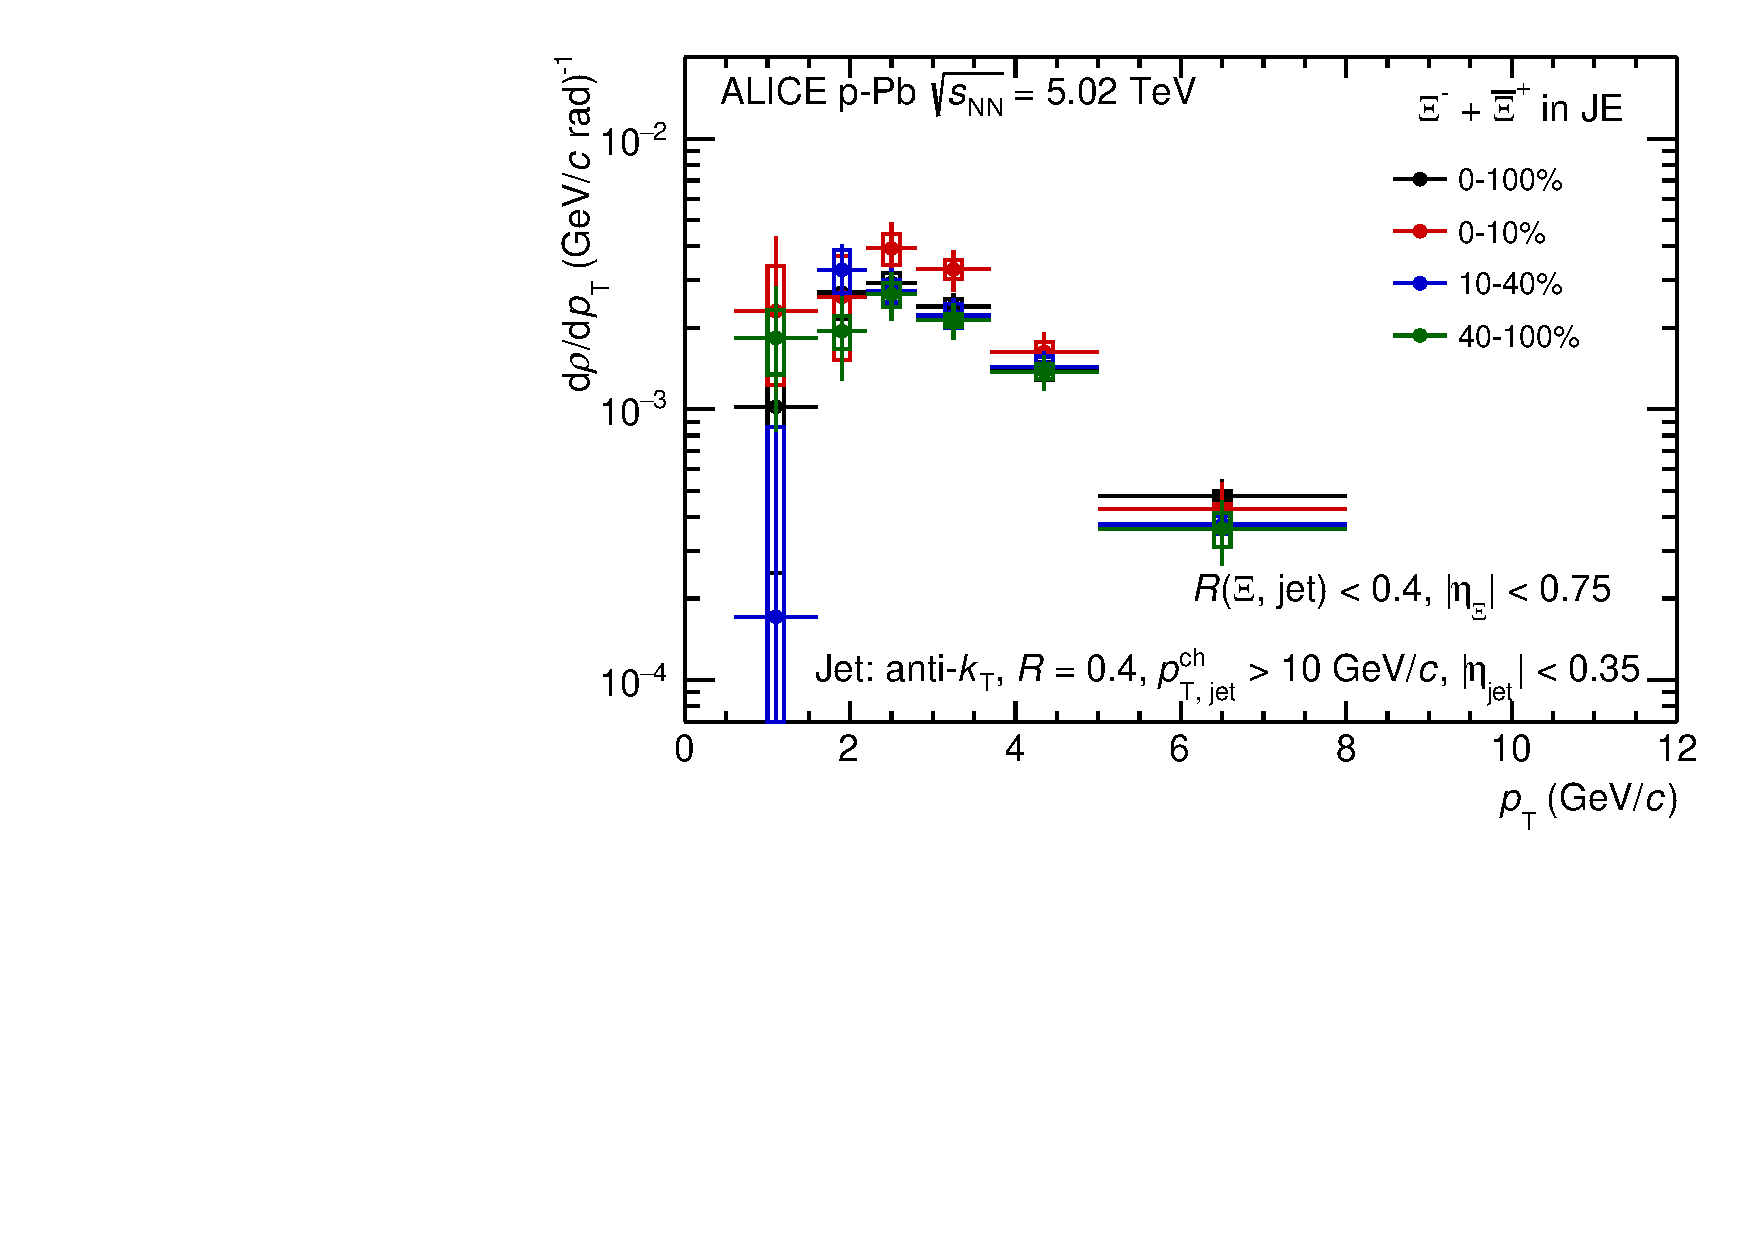
\includegraphics[width=.3\textwidth]{cf06_6}
	\end{center}
	\caption{$\pT$-differential density of $\kzero$, $\lmb + \almb$ and $\X + \Ix$ in different V0A event centrality classes in \pPb at \fivenn. Top panels show the inclusive particle and bottom panels show particles generated by jet fragmentation. The different centrality classes are depicted with different color.}
	\label{fig:pPbSpectwCent}
\end{figure}

\subsection{Baryon-to-meson and baryon-to-baryon ratios}
\label{subsec:ParRatios}
The $\lmb/\kzero$, $\Xi/\kzero$ and $\Omega/\kzero$ baryon-to-meson ratios and $\Xi/\lmb$, $\Omega/\lmb$ and $\Omega/\Xi$ baryon-to-baryon ratios are investigated as a function of $\pT$ for several selections in \pp and \pPb collisions. As can be seen in Figs.~\ref{fig:ppRatio} (\pp at \thirteen) and \ref{fig:pPbRatio} (\pPb at \fivenn, 0-100\%), the inclusive particle ratios have an enhancement at $\pT \sim 3 - 4 $~\GeVc. Additionally, the same case of particle ratios in underlying events can be observed. However, the particle ratios in jet are significantly lower than the inclusive and UE cases at low and intermediate $\pT$. Also the ratios in jet are approximately independent of $\pT$ beyond 2~\GeVc. This suggests that the ratios of baryon-to-meson and baryon-to-baryon enhancement at intermediate $\pT$ is not driven by the jet fragmentation.

\begin{figure}[!ht]
	\begin{center}
		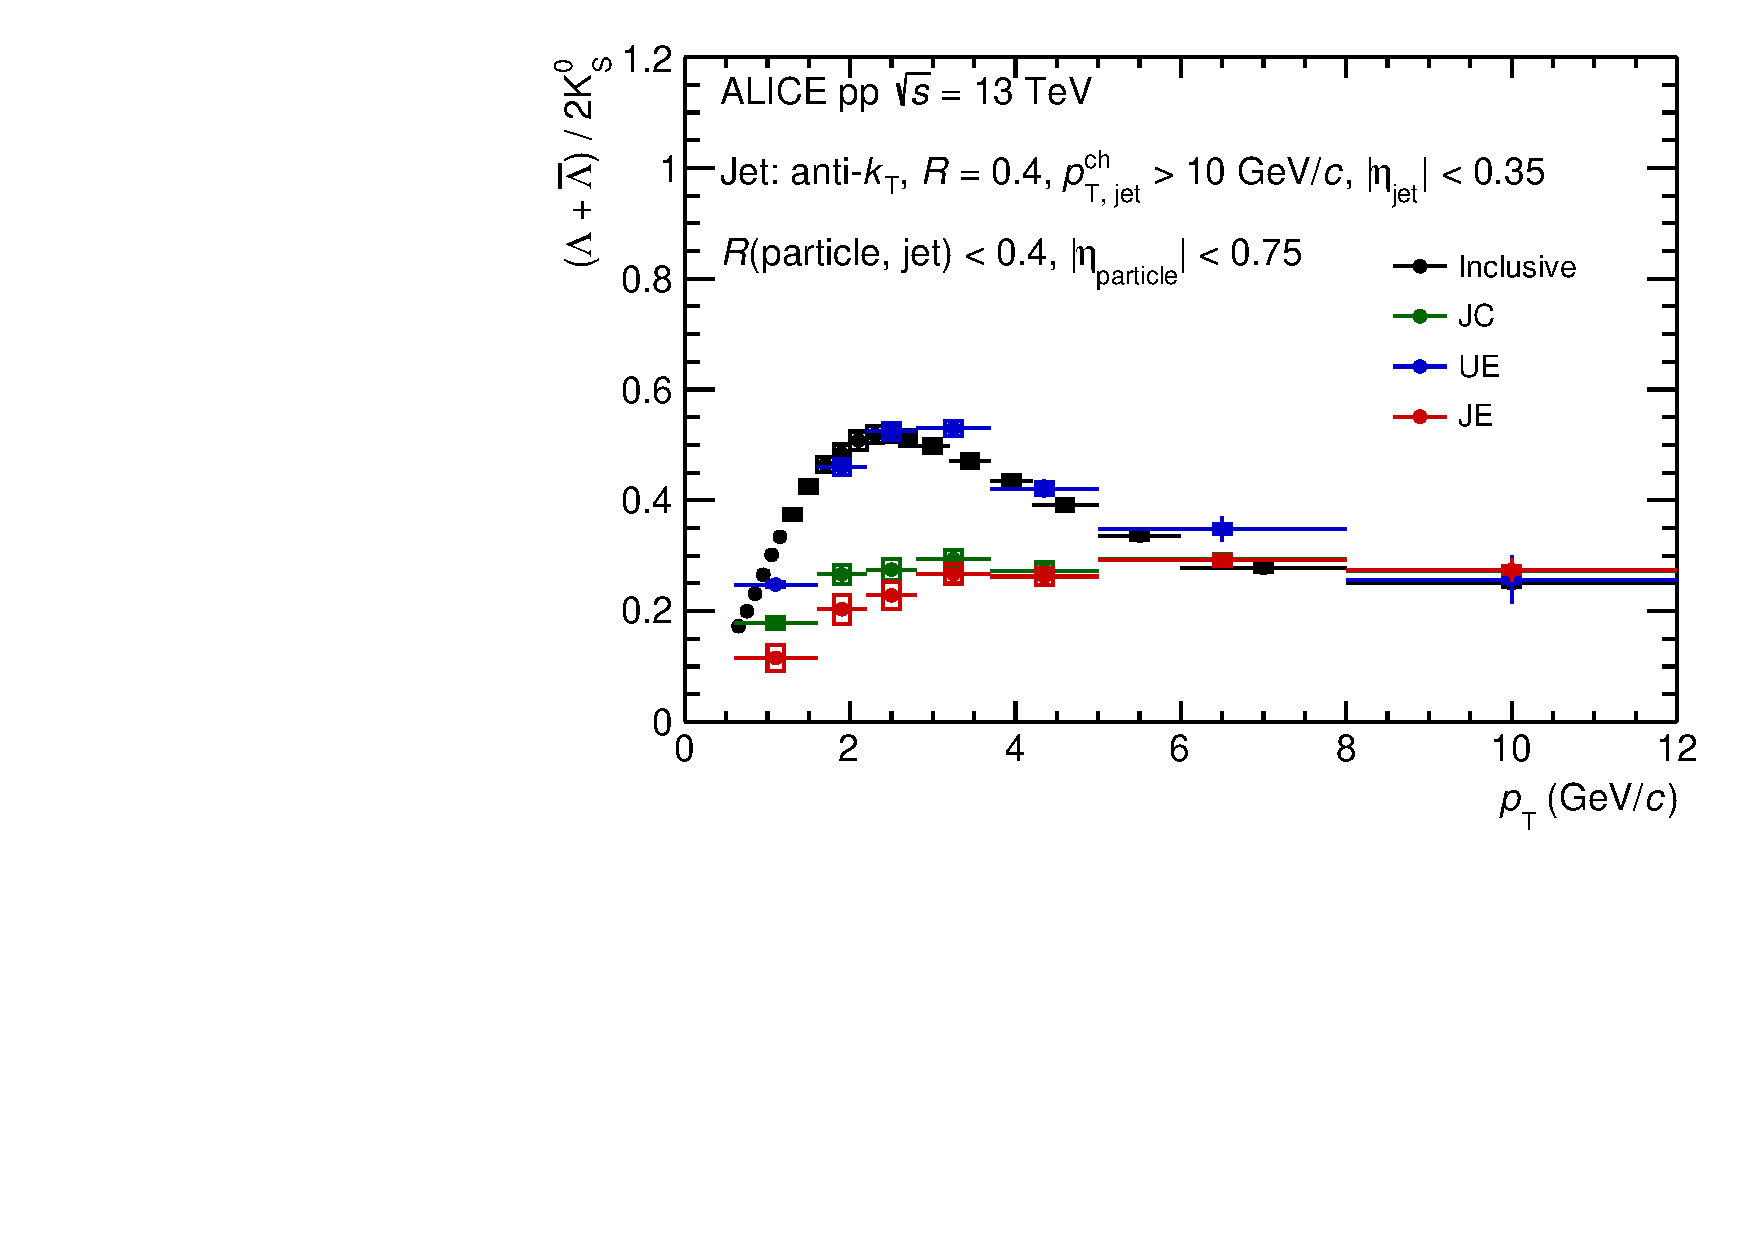
\includegraphics[width=.3\textwidth]{cf07_1}
		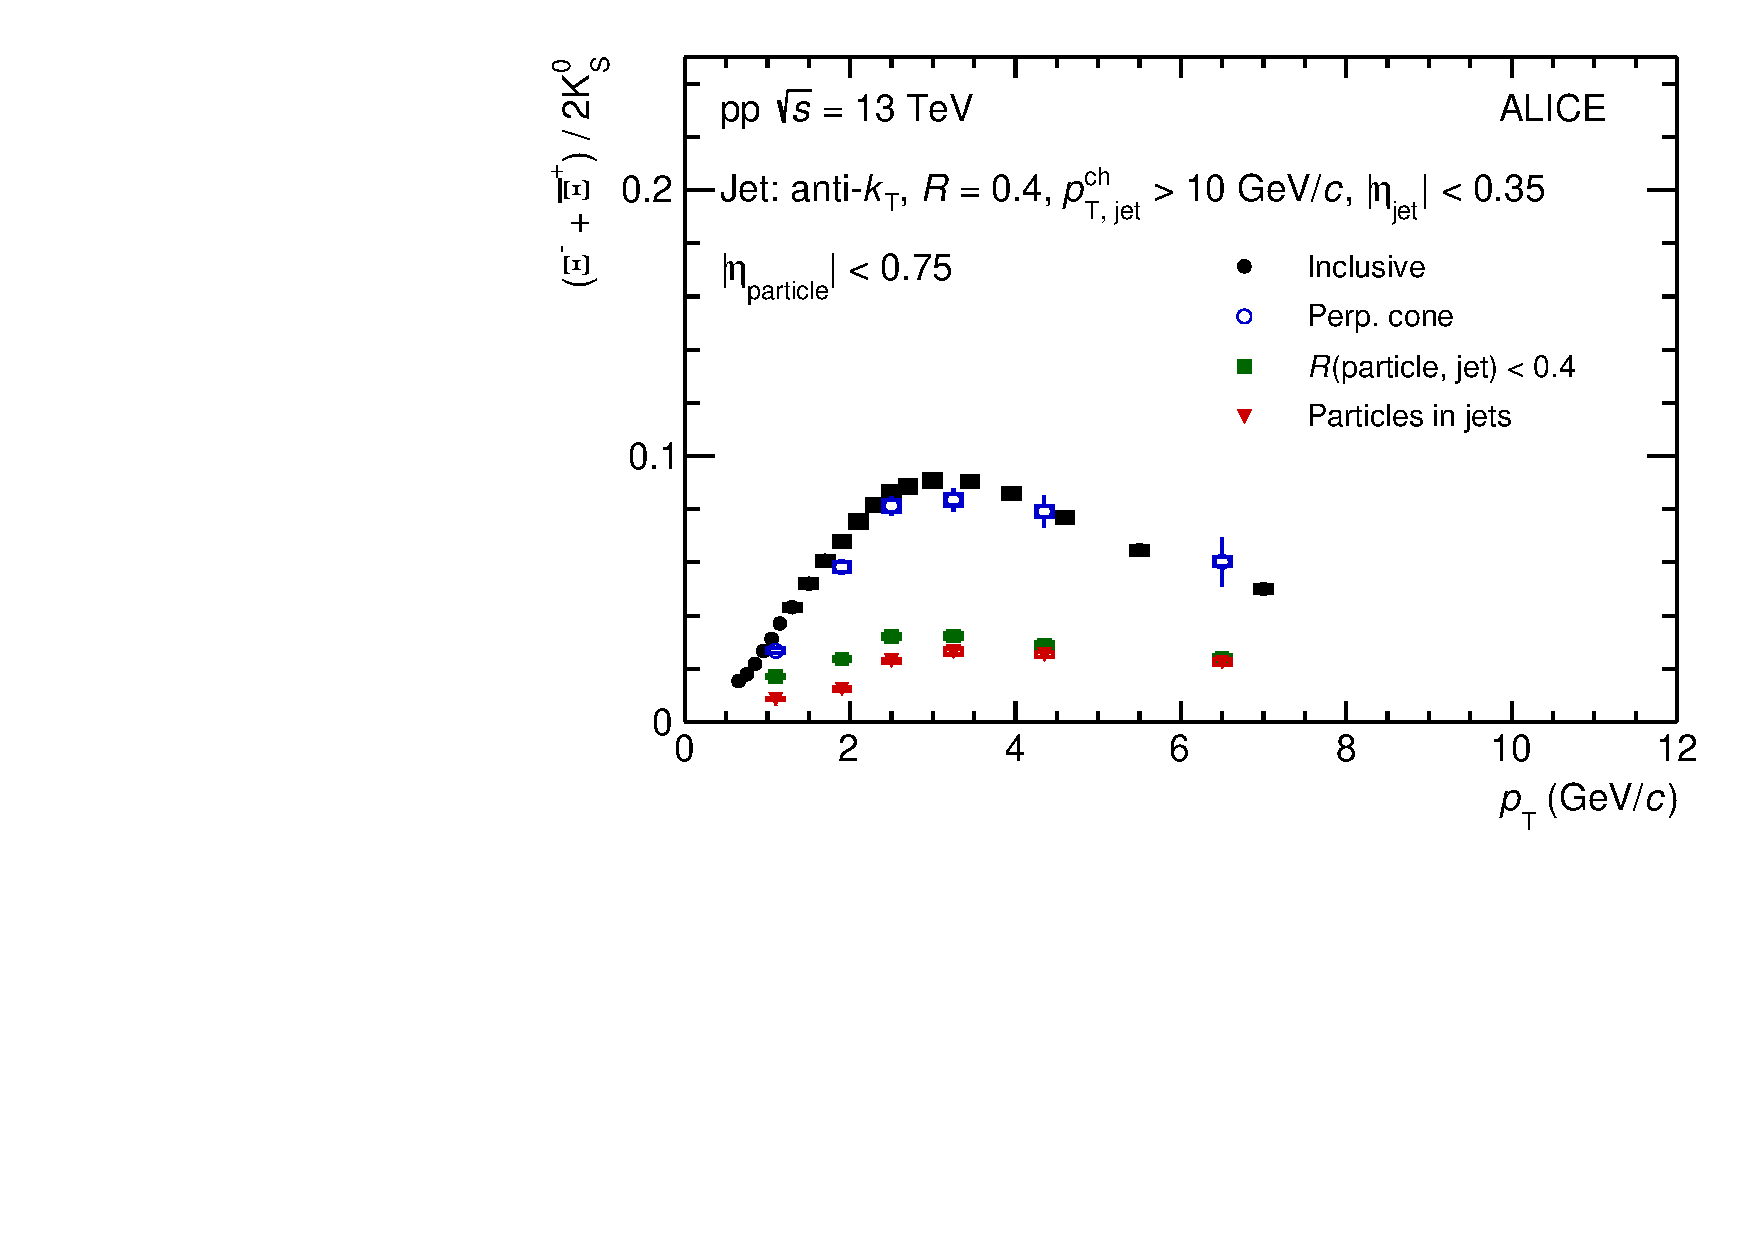
\includegraphics[width=.3\textwidth]{cf07_2}
		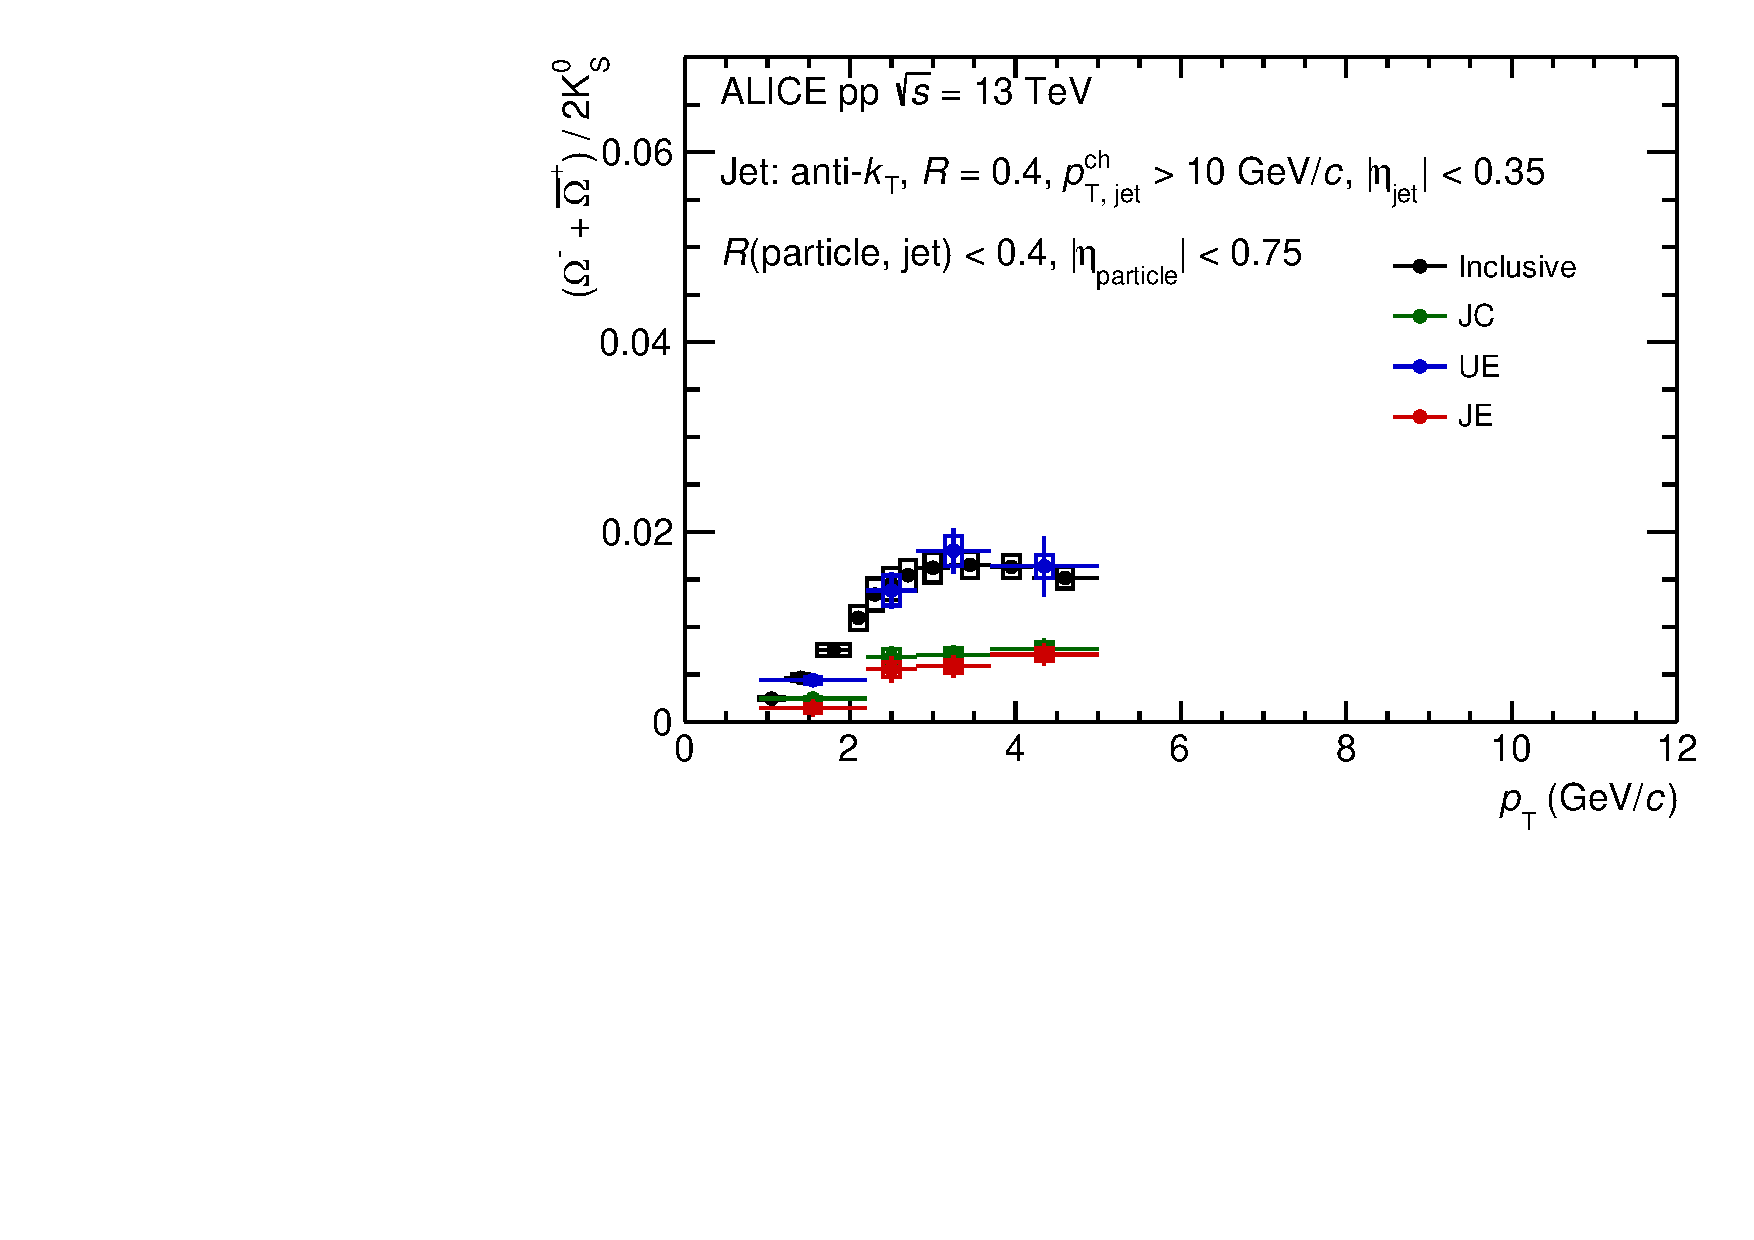
\includegraphics[width=.3\textwidth]{cf07_3}
		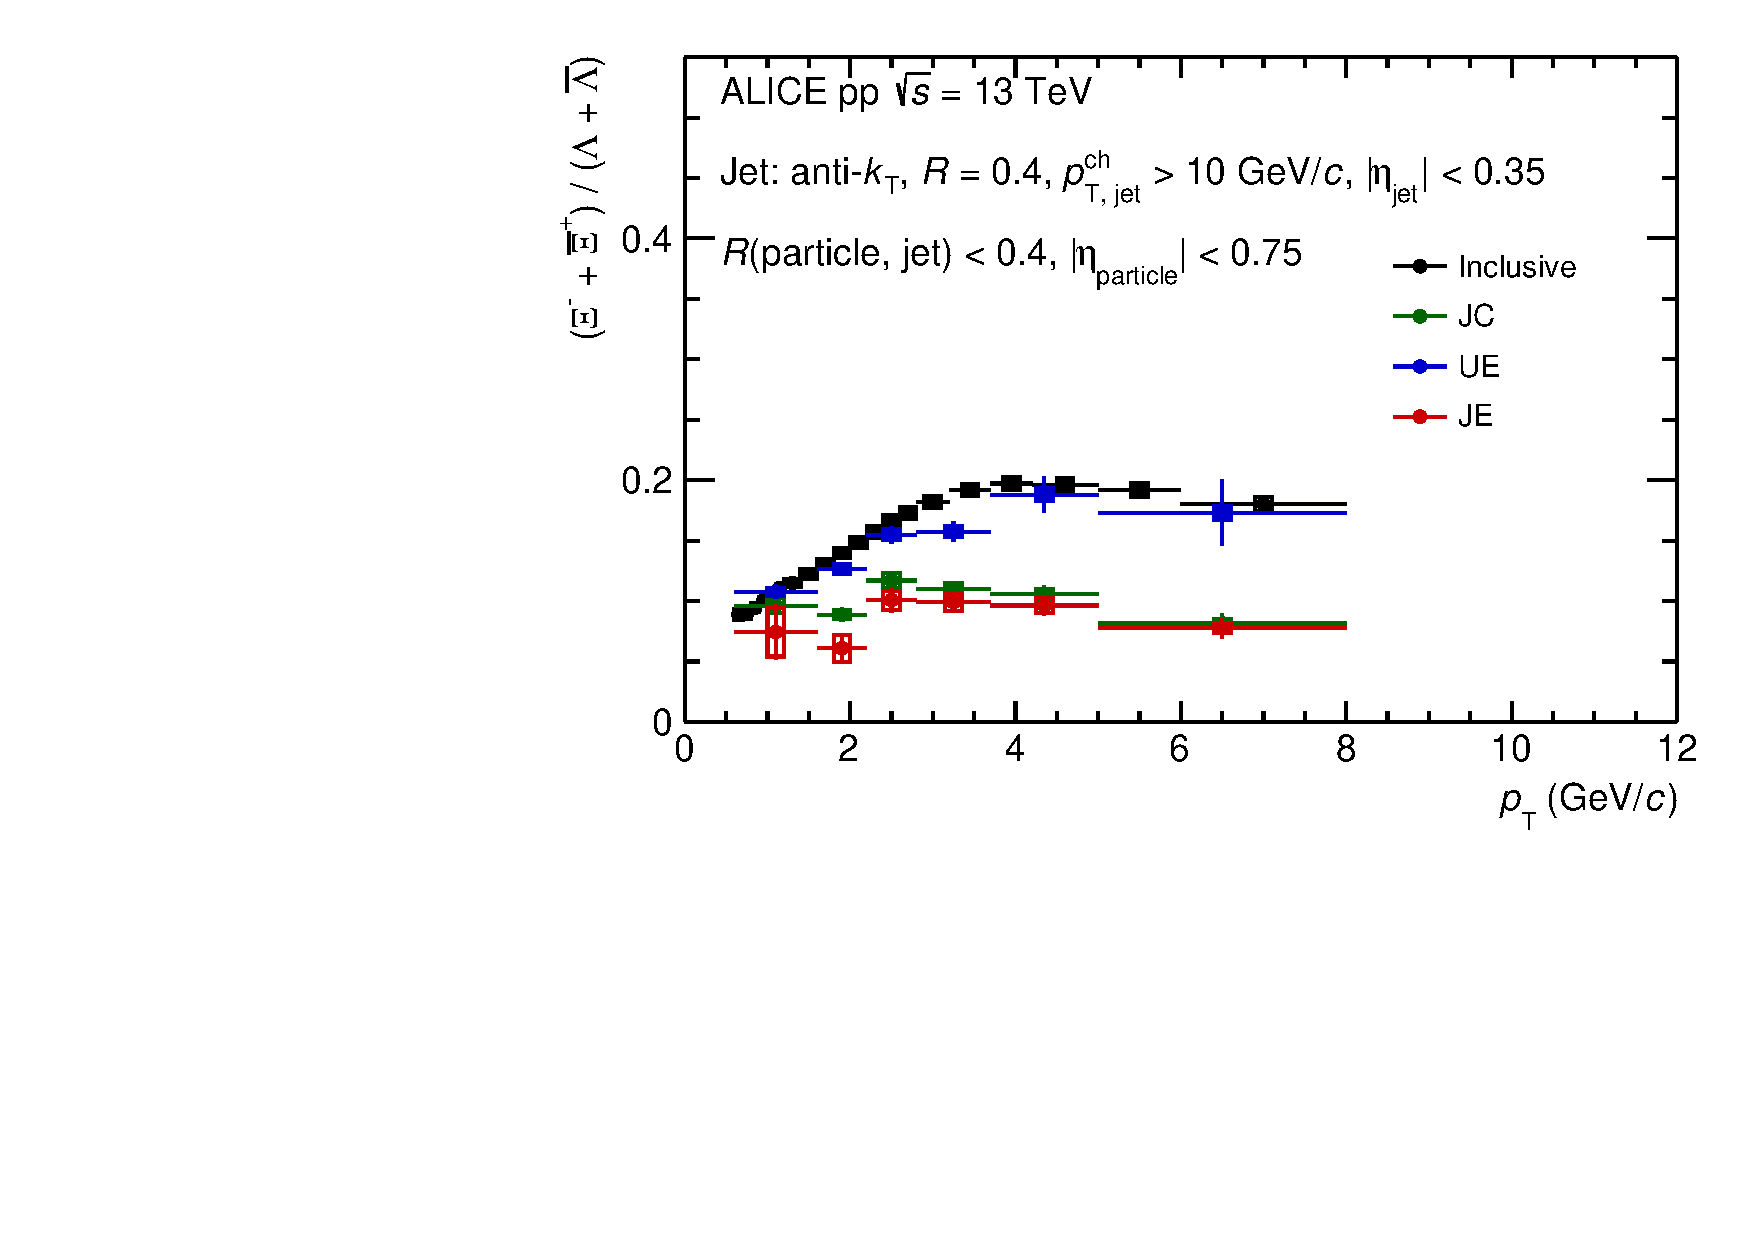
\includegraphics[width=.3\textwidth]{cf07_4}
		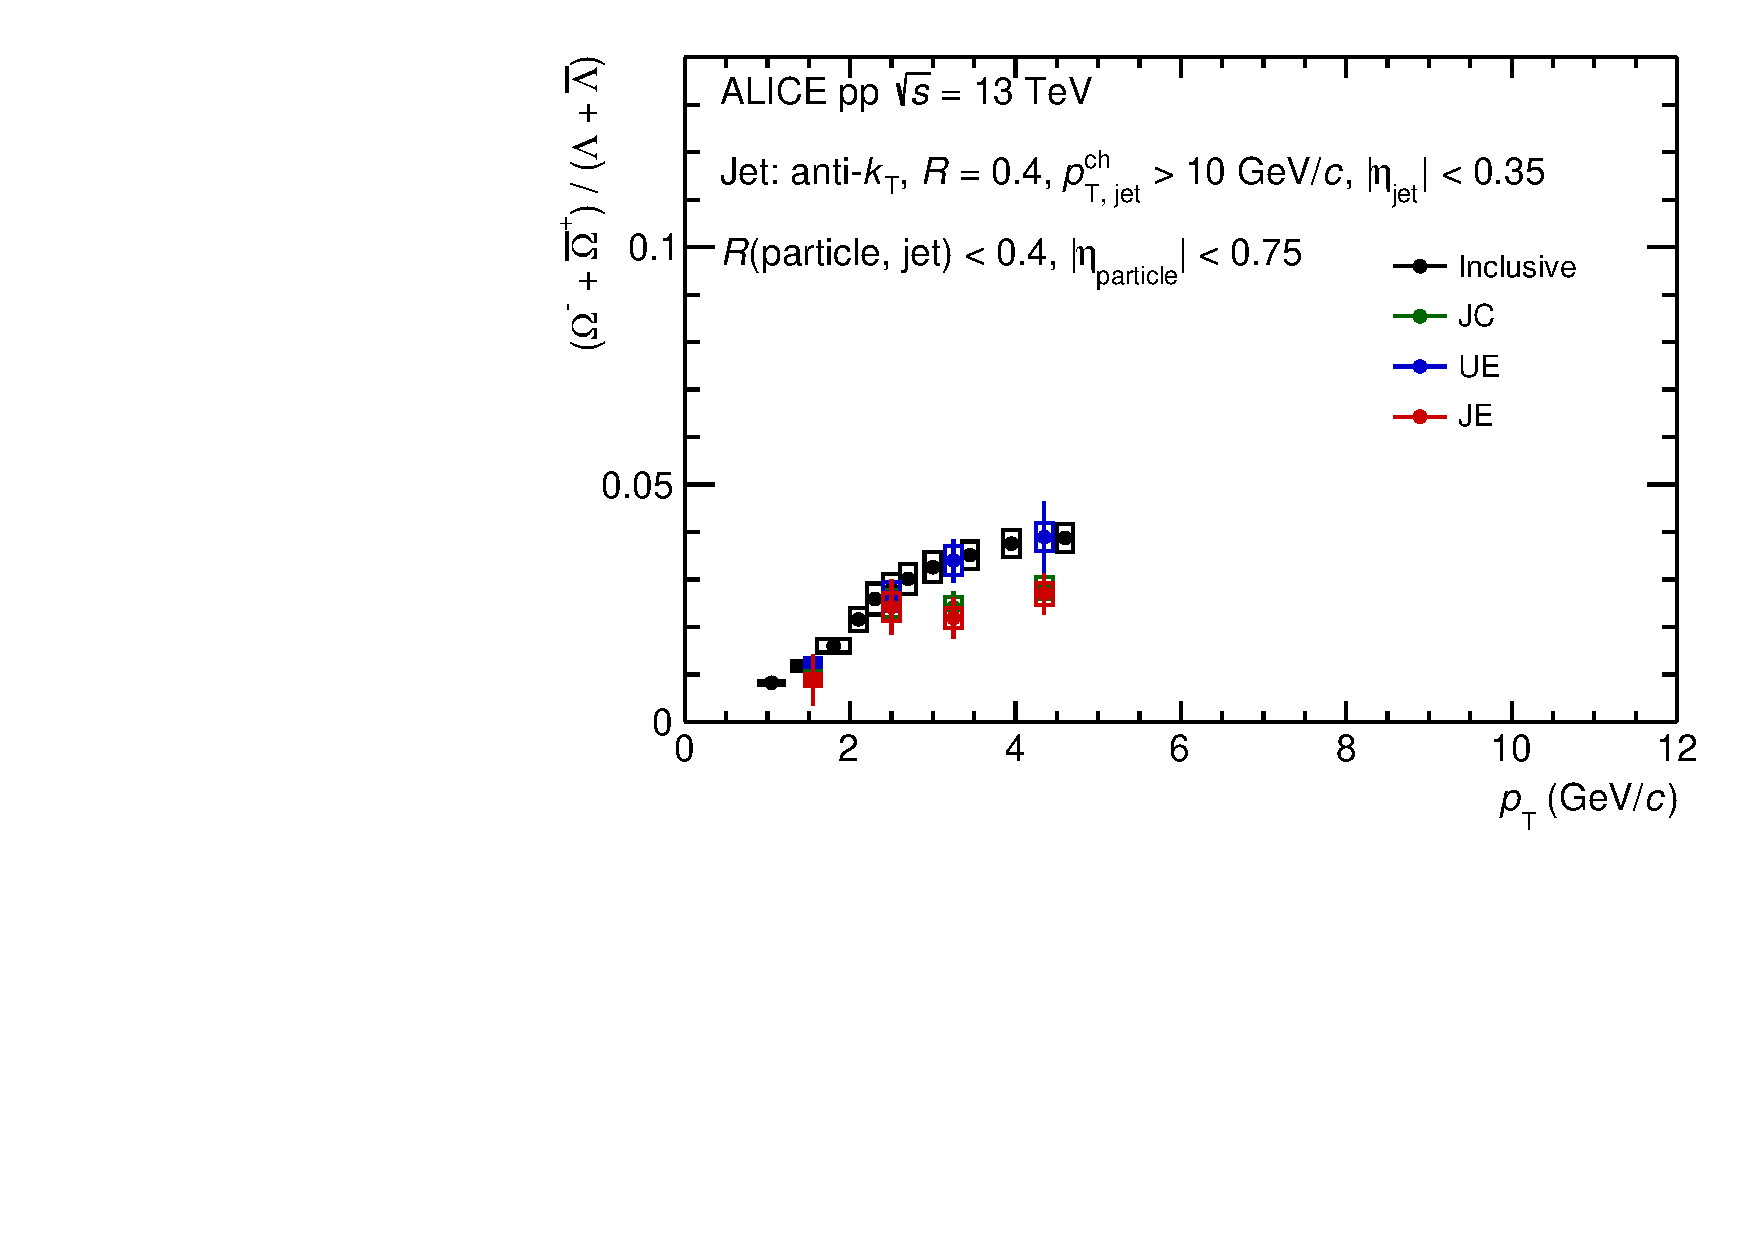
\includegraphics[width=.3\textwidth]{cf07_5}
		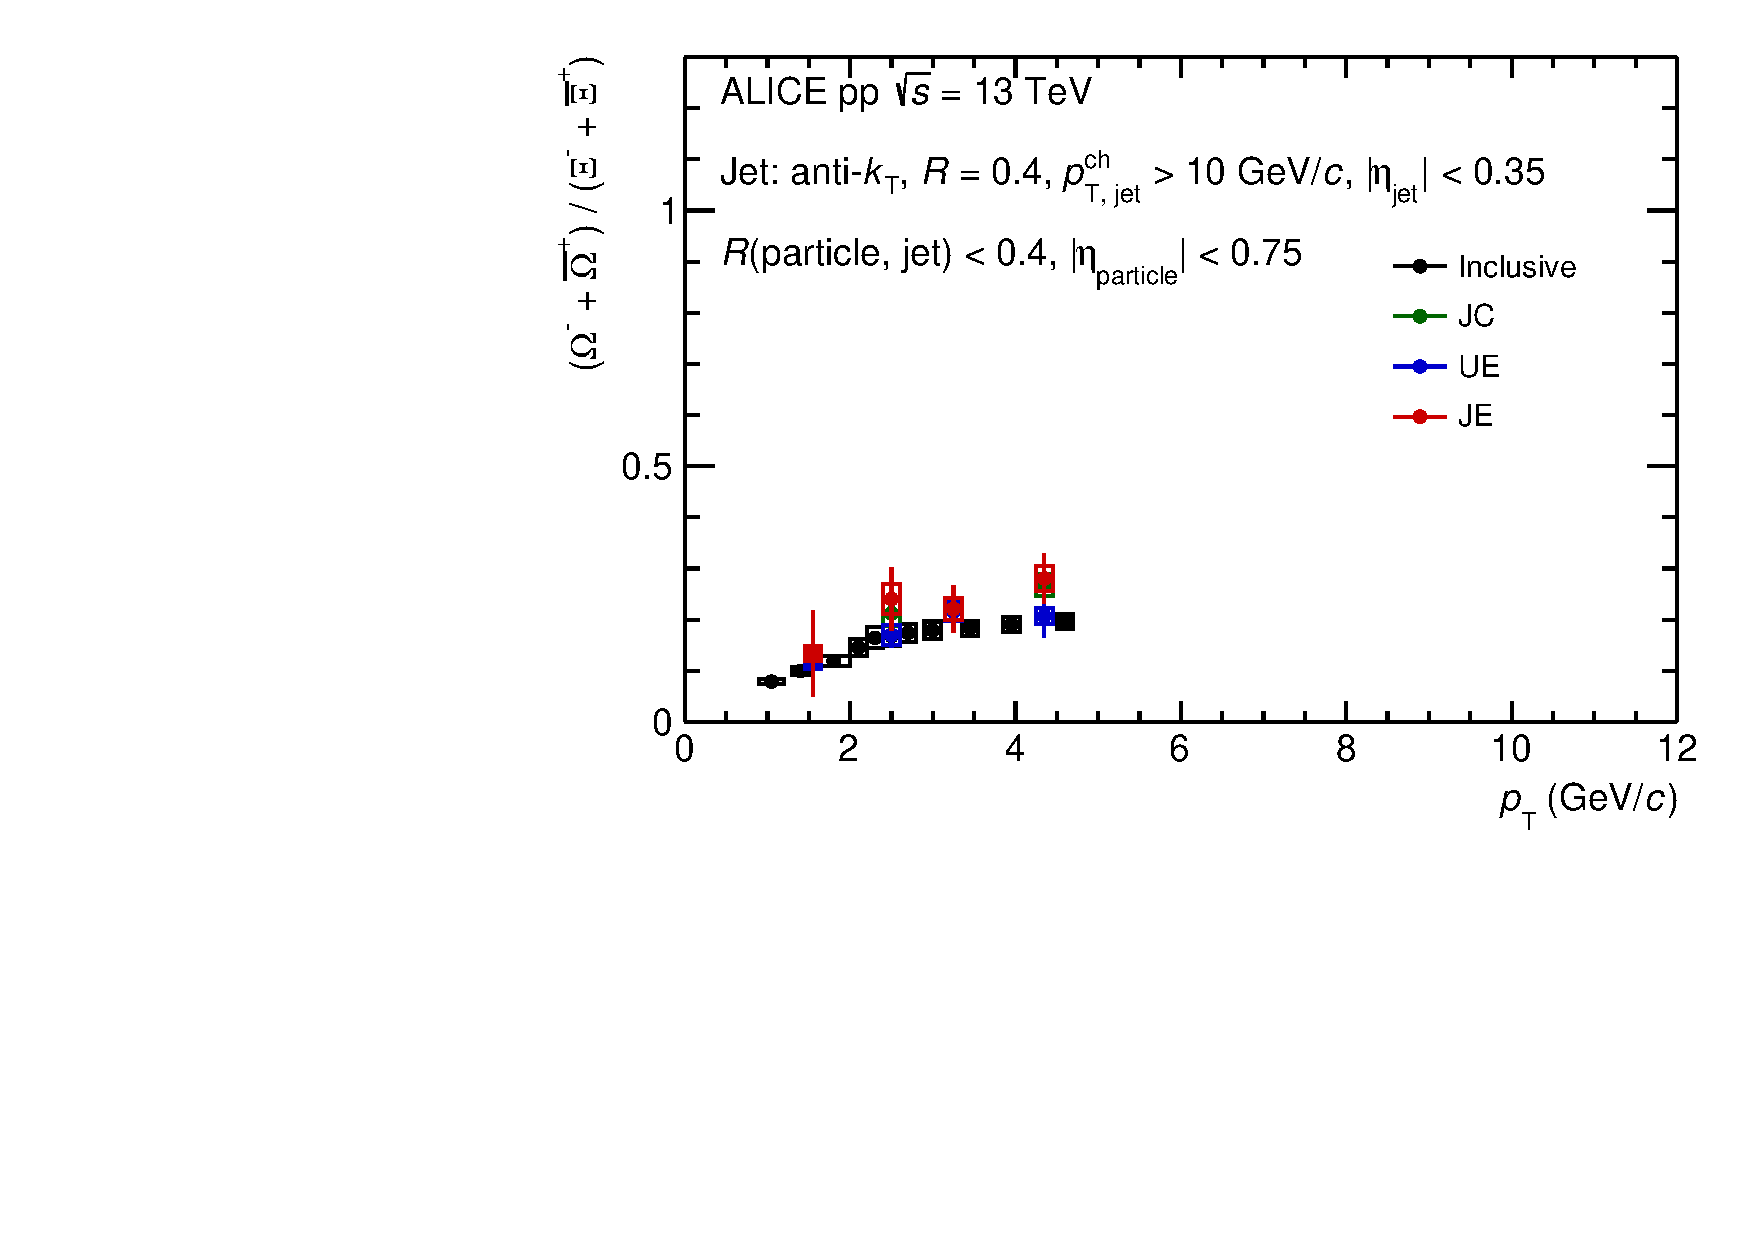
\includegraphics[width=.3\textwidth]{cf07_6}
	\end{center}
	\caption{The baryon-to-meson (top) and baryon-to-baryon(bottom) ratio as a function of particle $\pT$ in \pp collisions at \thirteen. In those panels, the black point shows the ratio with particles from minimum bias events, the green point shows the ratio with particles from the jet cones, the blue point shows the ratio with particles from perpendicular cones with jet and the red point shows the ratio with particles that generated by jet.}
	\label{fig:ppRatio}
\end{figure}
\begin{figure}[!ht]
	\begin{center}
		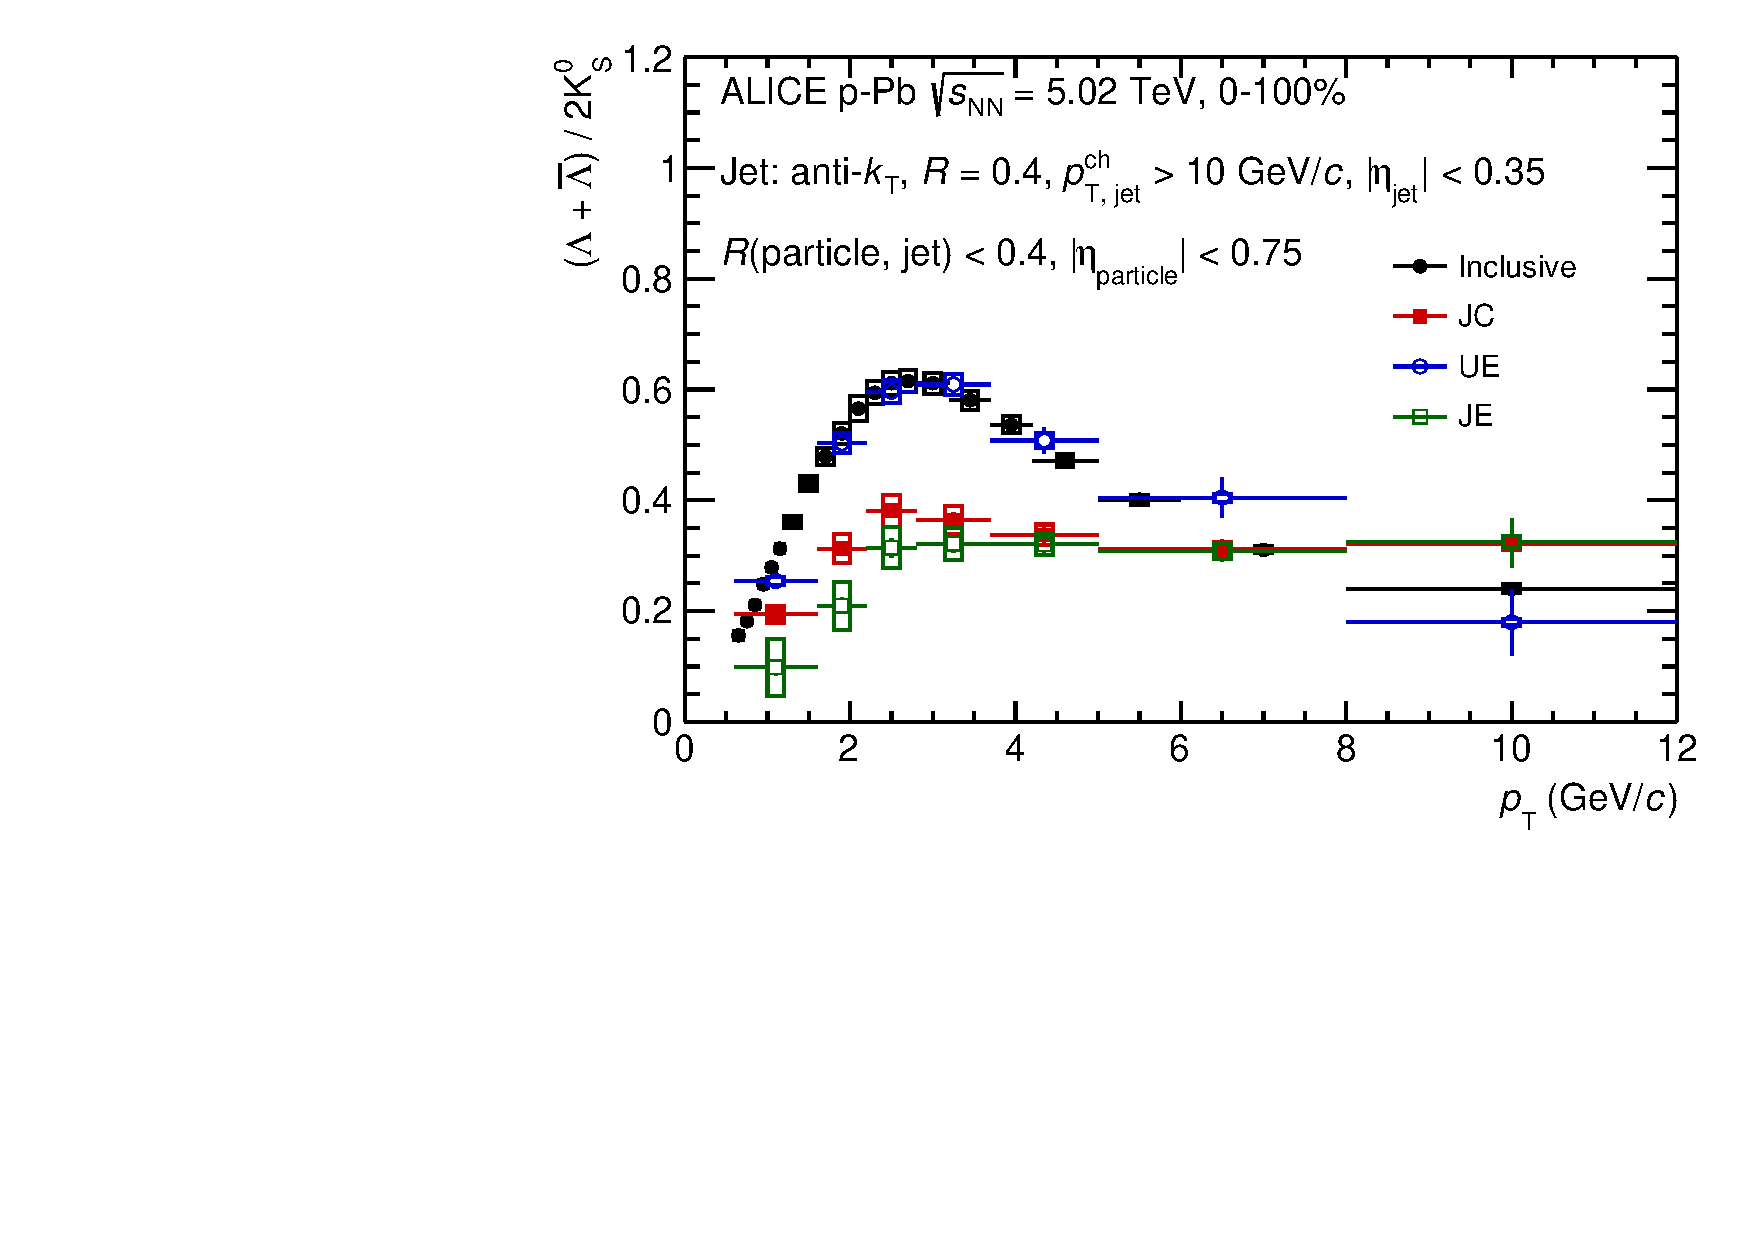
\includegraphics[width=.3\textwidth]{cf08_1}
		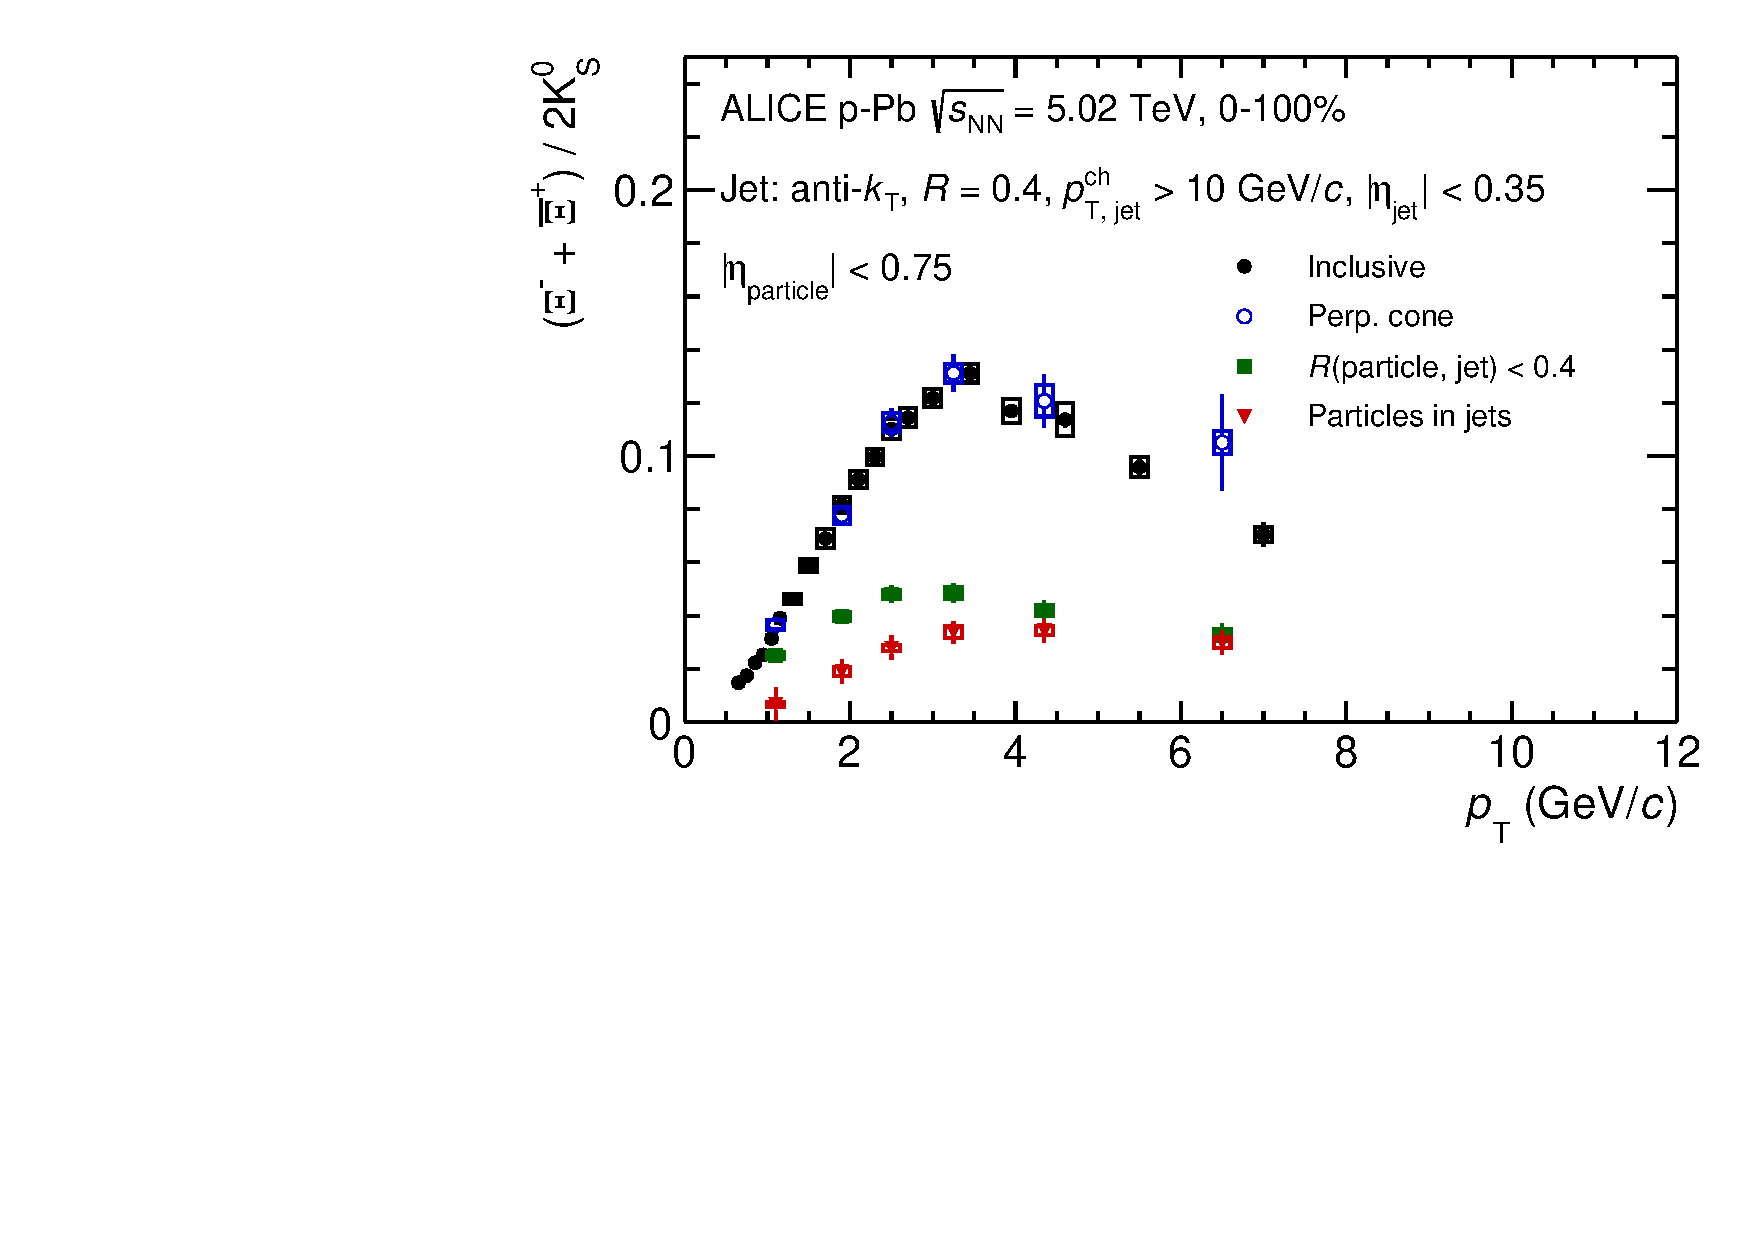
\includegraphics[width=.3\textwidth]{cf08_2}
		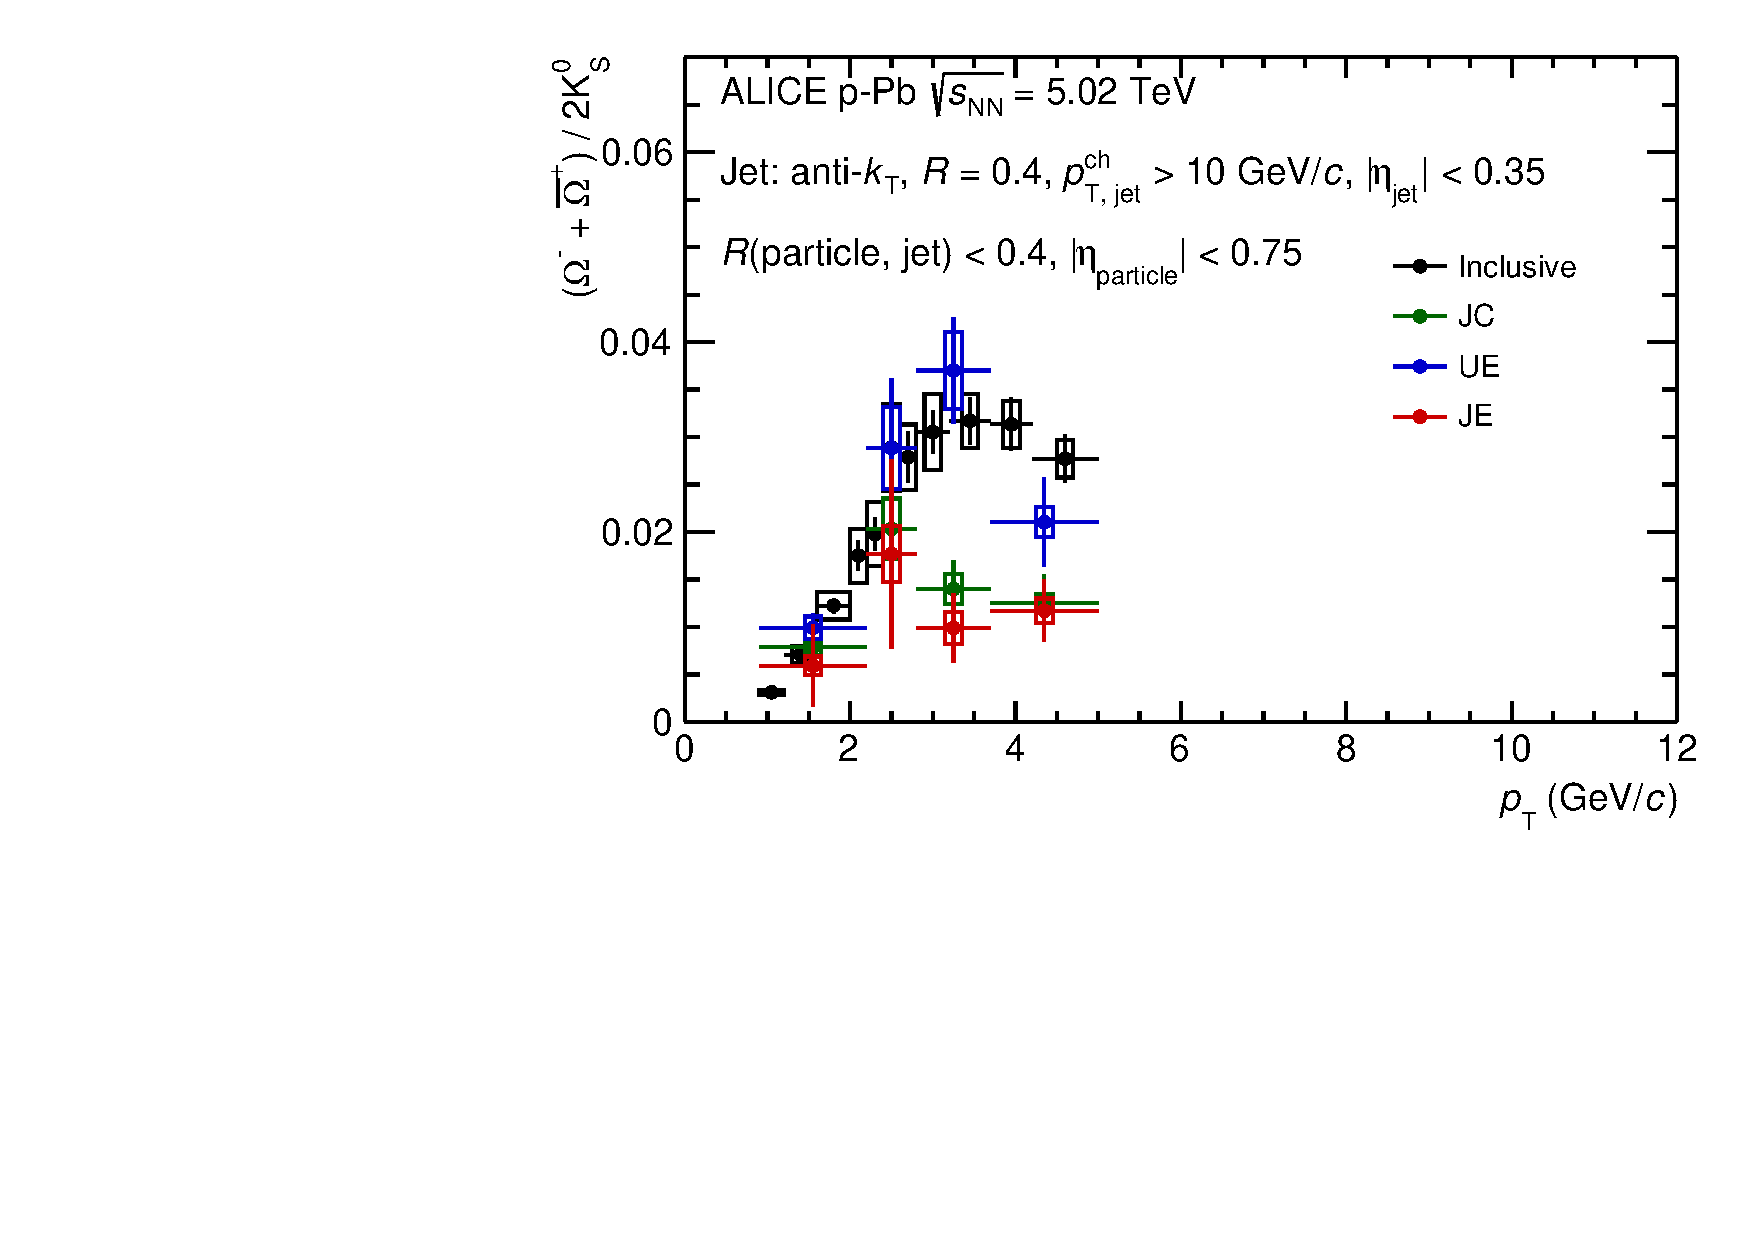
\includegraphics[width=.3\textwidth]{cf08_3}
		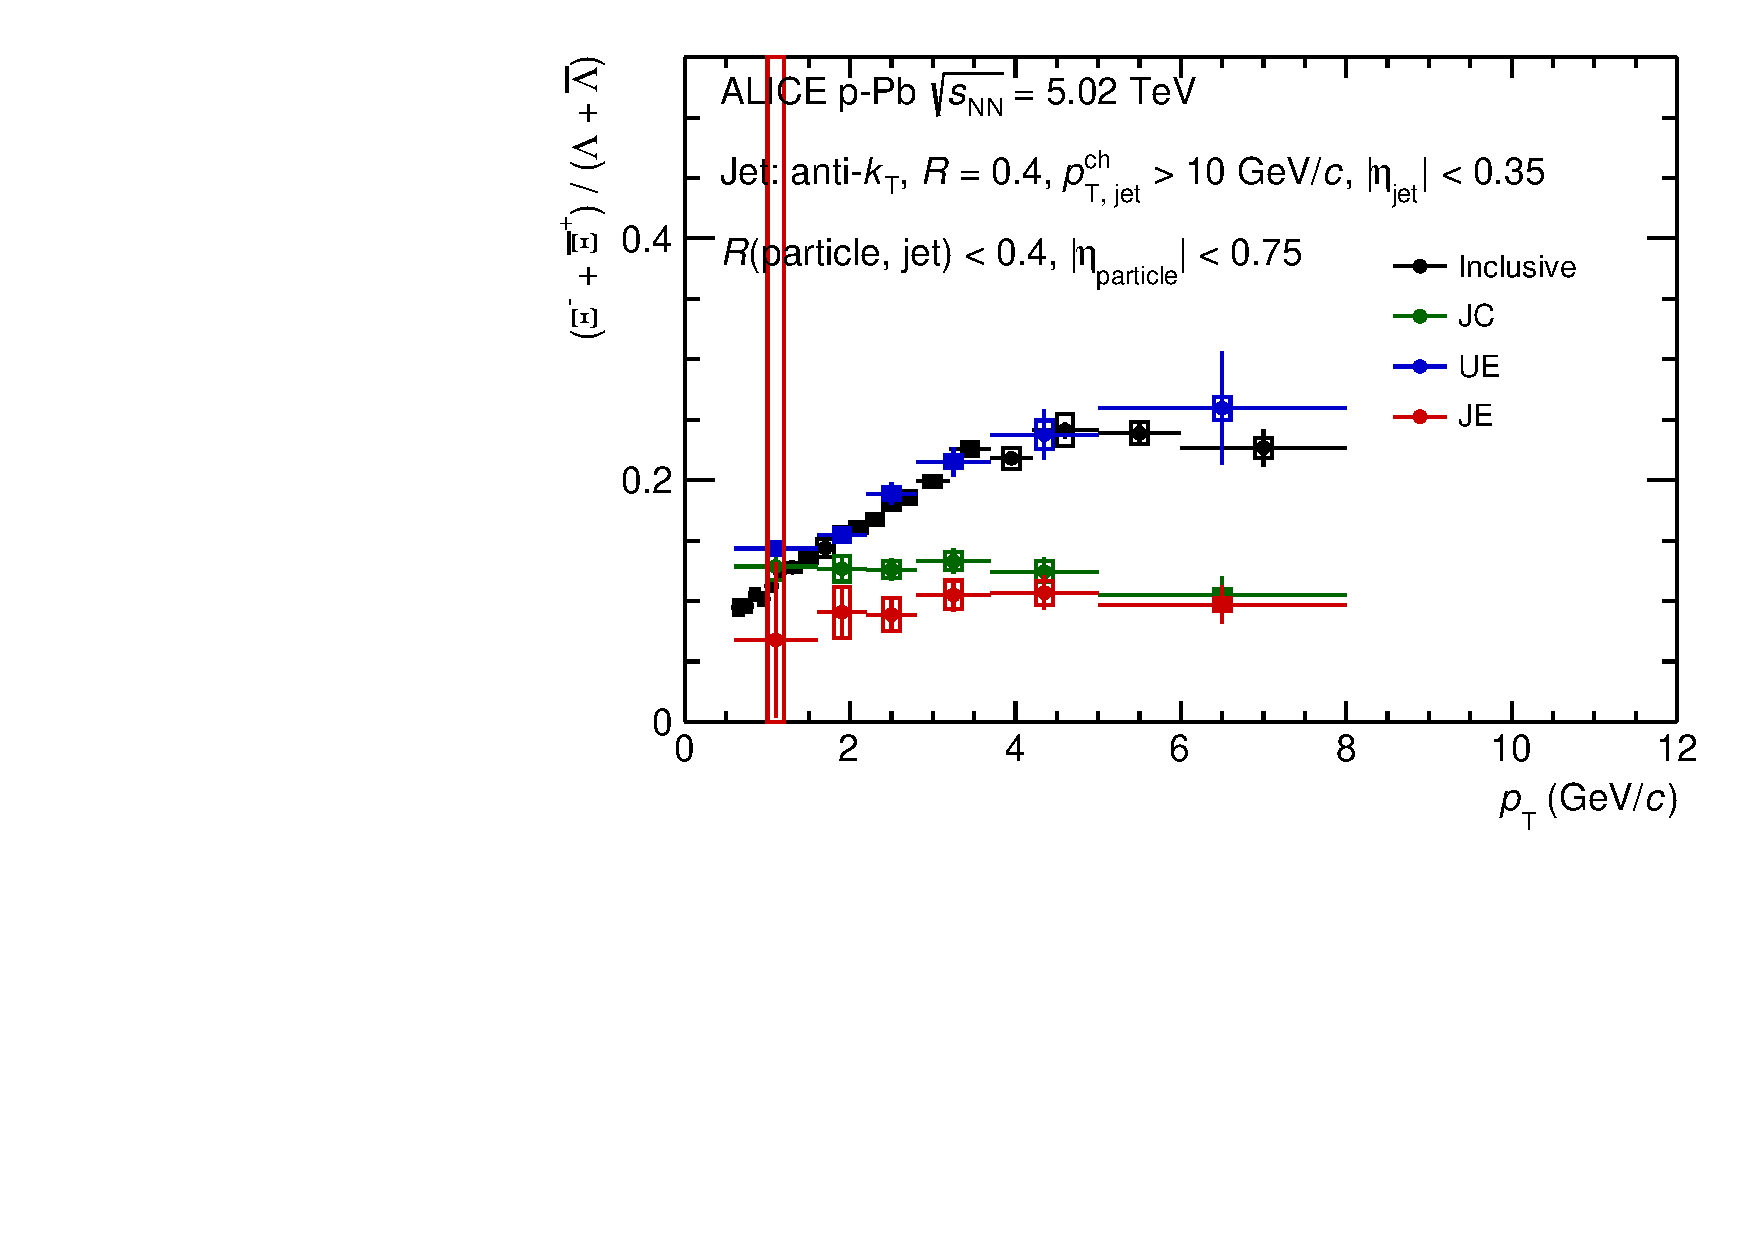
\includegraphics[width=.3\textwidth]{cf08_4}
		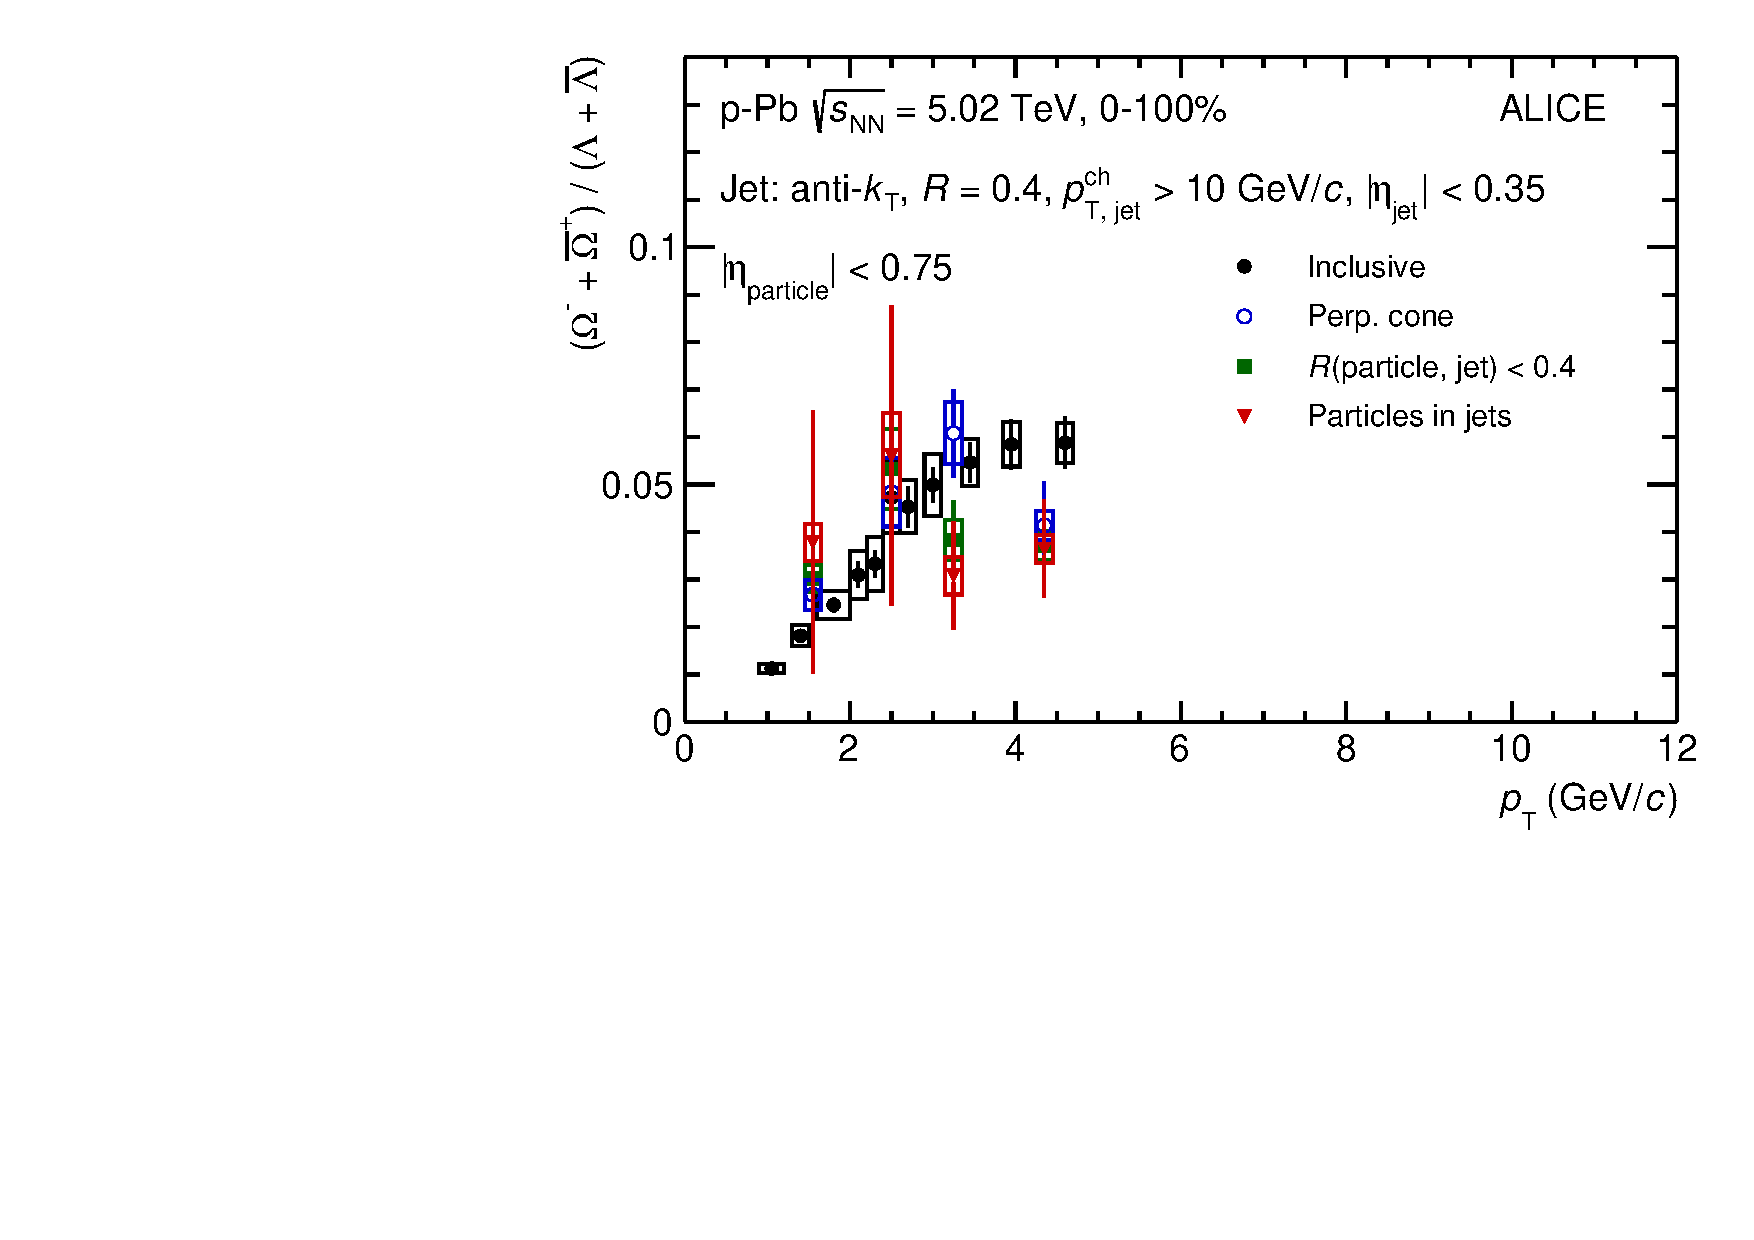
\includegraphics[width=.3\textwidth]{cf08_5}
		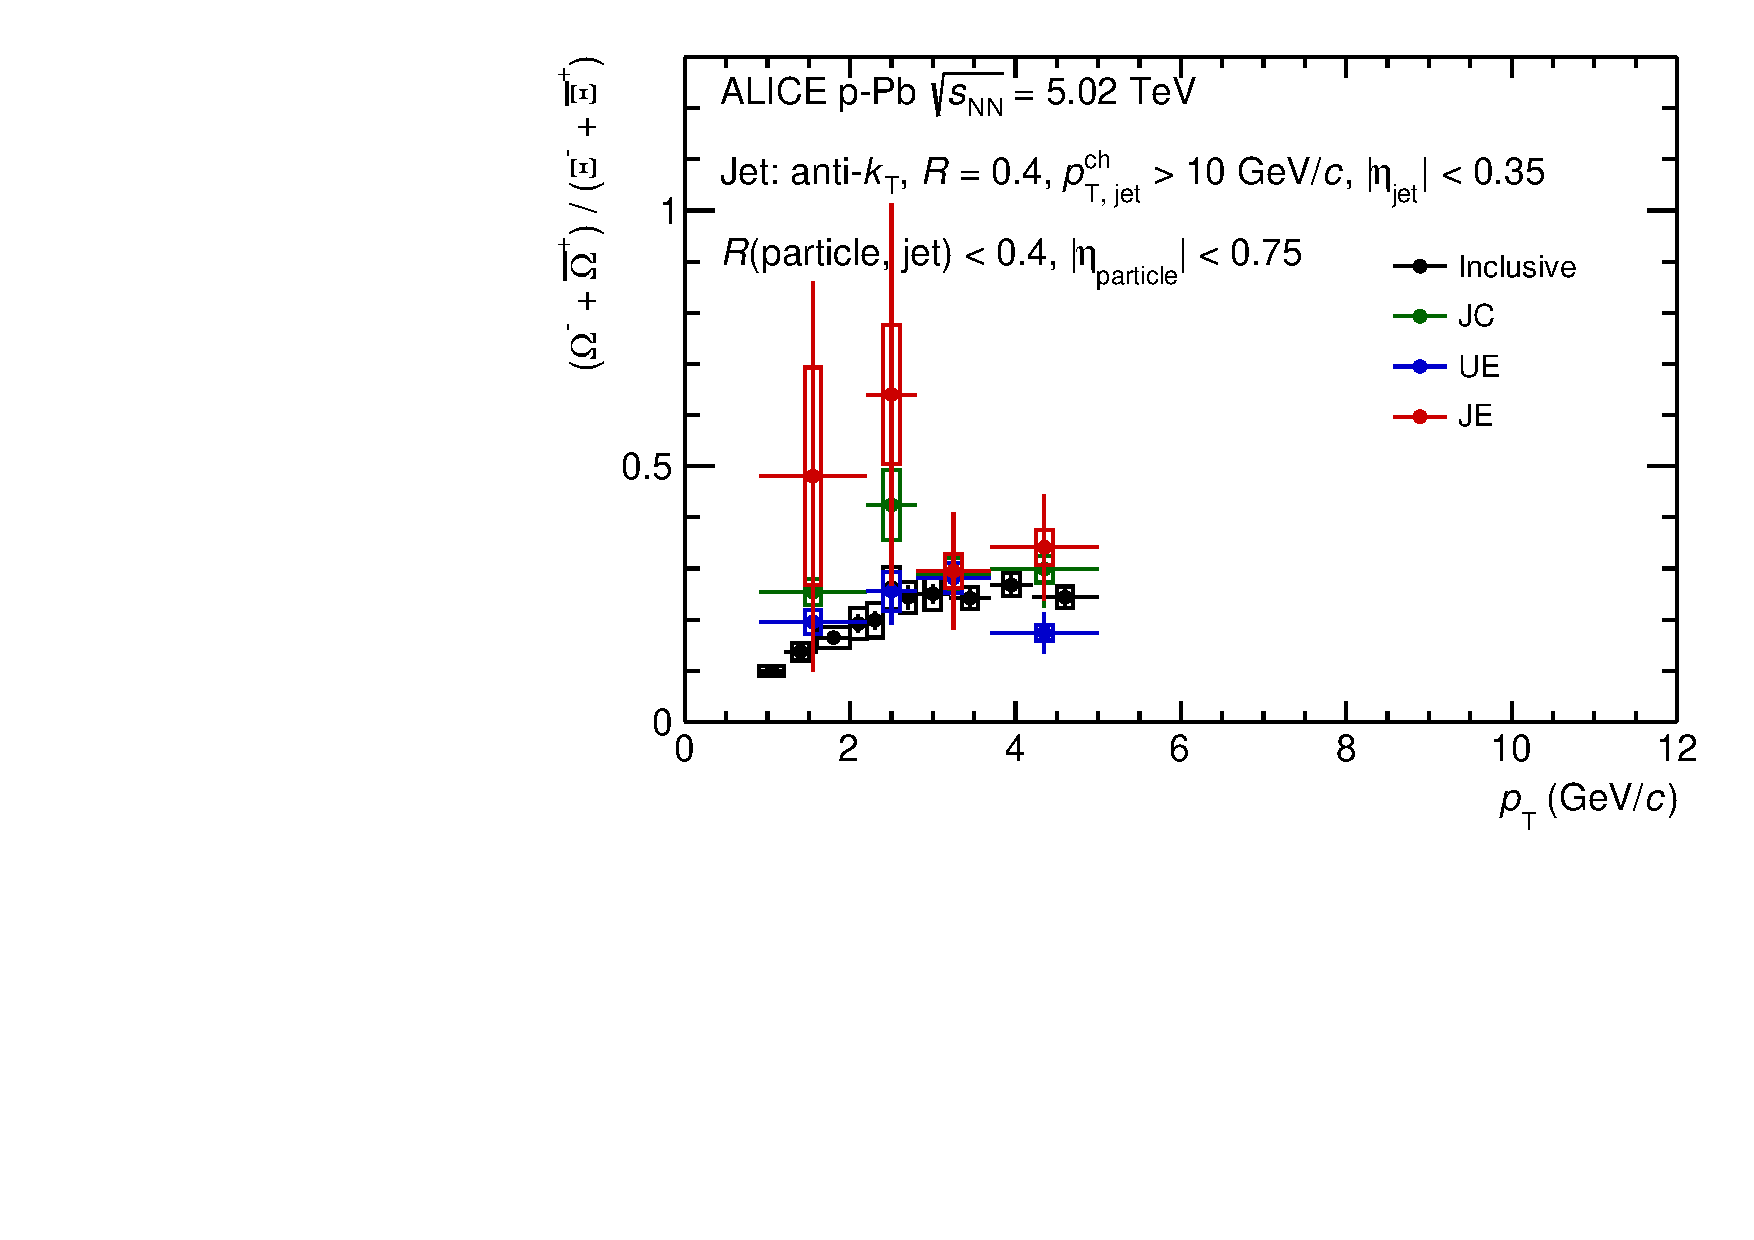
\includegraphics[width=.3\textwidth]{cf08_6}
	\end{center}
	\caption{The baryon-to-meson (top) and baryon-to-baryon(bottom) ratio as a function of particle $\pT$ in \pPb collisions at \fivenn. In those panels, the black point shows the ratio with particles from minimum bias events, the green point shows the ratio with particles from the jet cones, the blue point shows the ratio with particles from perpendicular cones with jet and the red point shows the ratio with particles that generated by jet.}
	\label{fig:pPbRatio}
\end{figure}

The particle ratios in jet with centrality and collision system distribution is studied in Fig.~\ref{fig:pppPbRatio}. The particle ratios in the jet are observed to be relatively centrality and system independent. It is noteworthy that the baryon-to-meson ($\lmb/\kzero$, $\Xi/\kzero$ and $\Omega/\kzero$) ratios have a hint of centrality (collision system) dependent for $2 < \pT < 4$~\GeVc, however this is barely significant given the quoted uncertainties. For $\pT > 5$~\GeVc, the baryon-to-meson ratios become fairly consistent for all centrality classes and collision systems. 

\begin{figure}[!ht]
	\begin{center}
		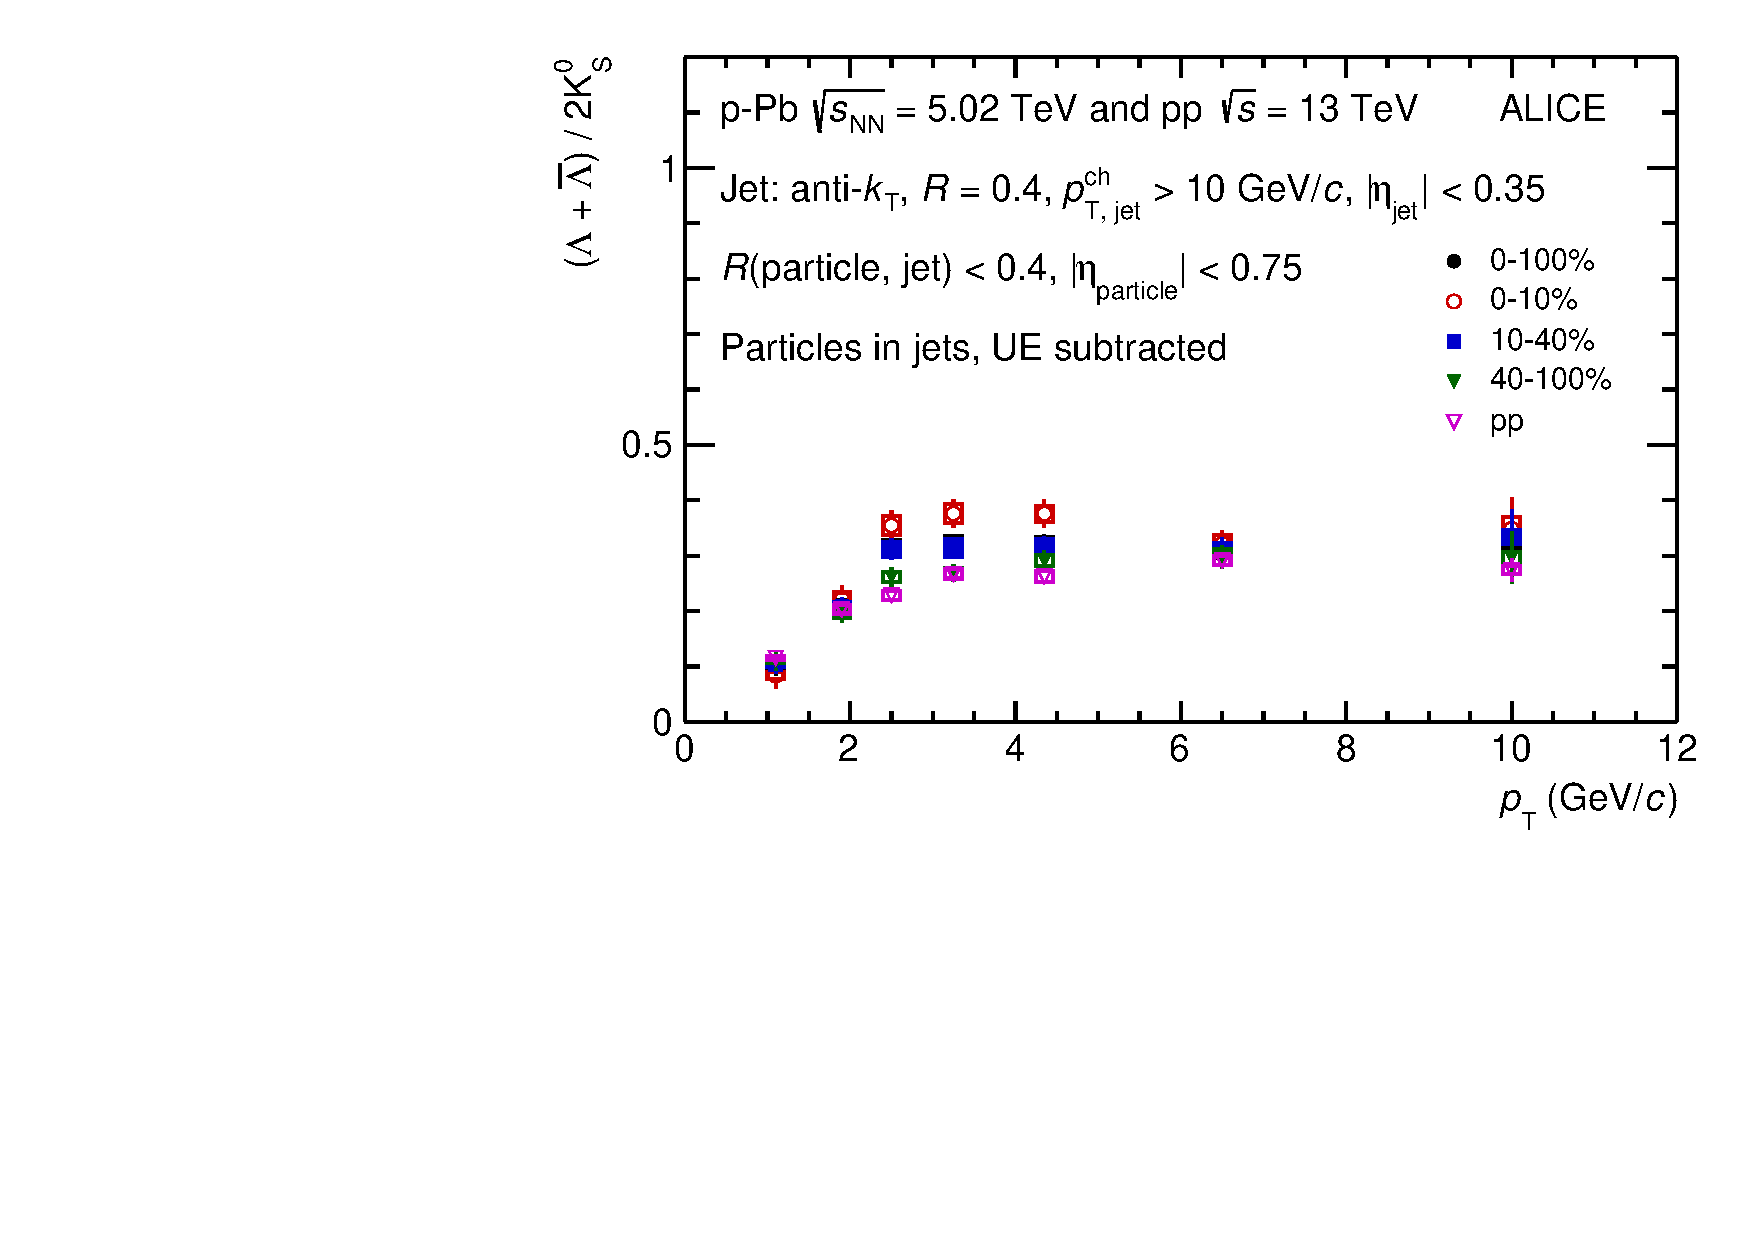
\includegraphics[width=.3\textwidth]{cf09_1}
		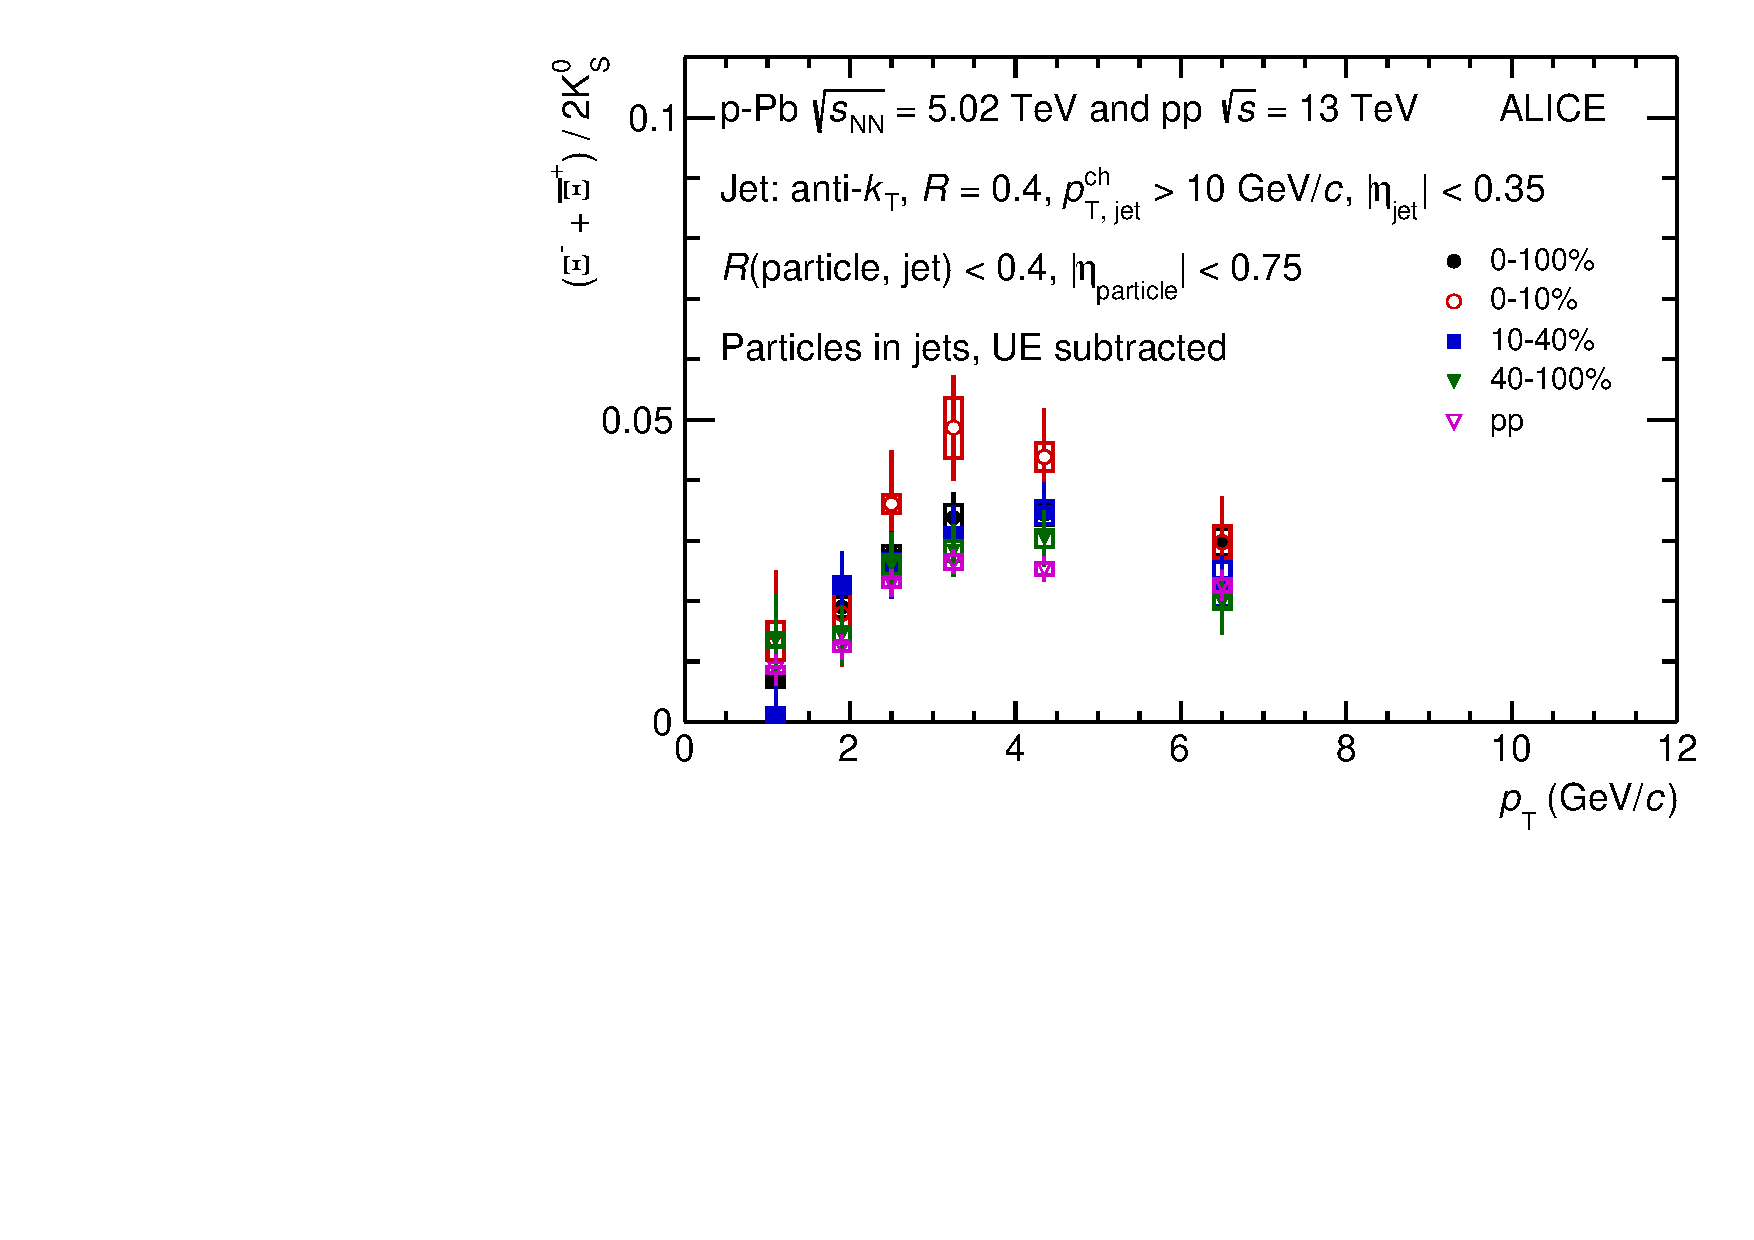
\includegraphics[width=.3\textwidth]{cf09_2}
		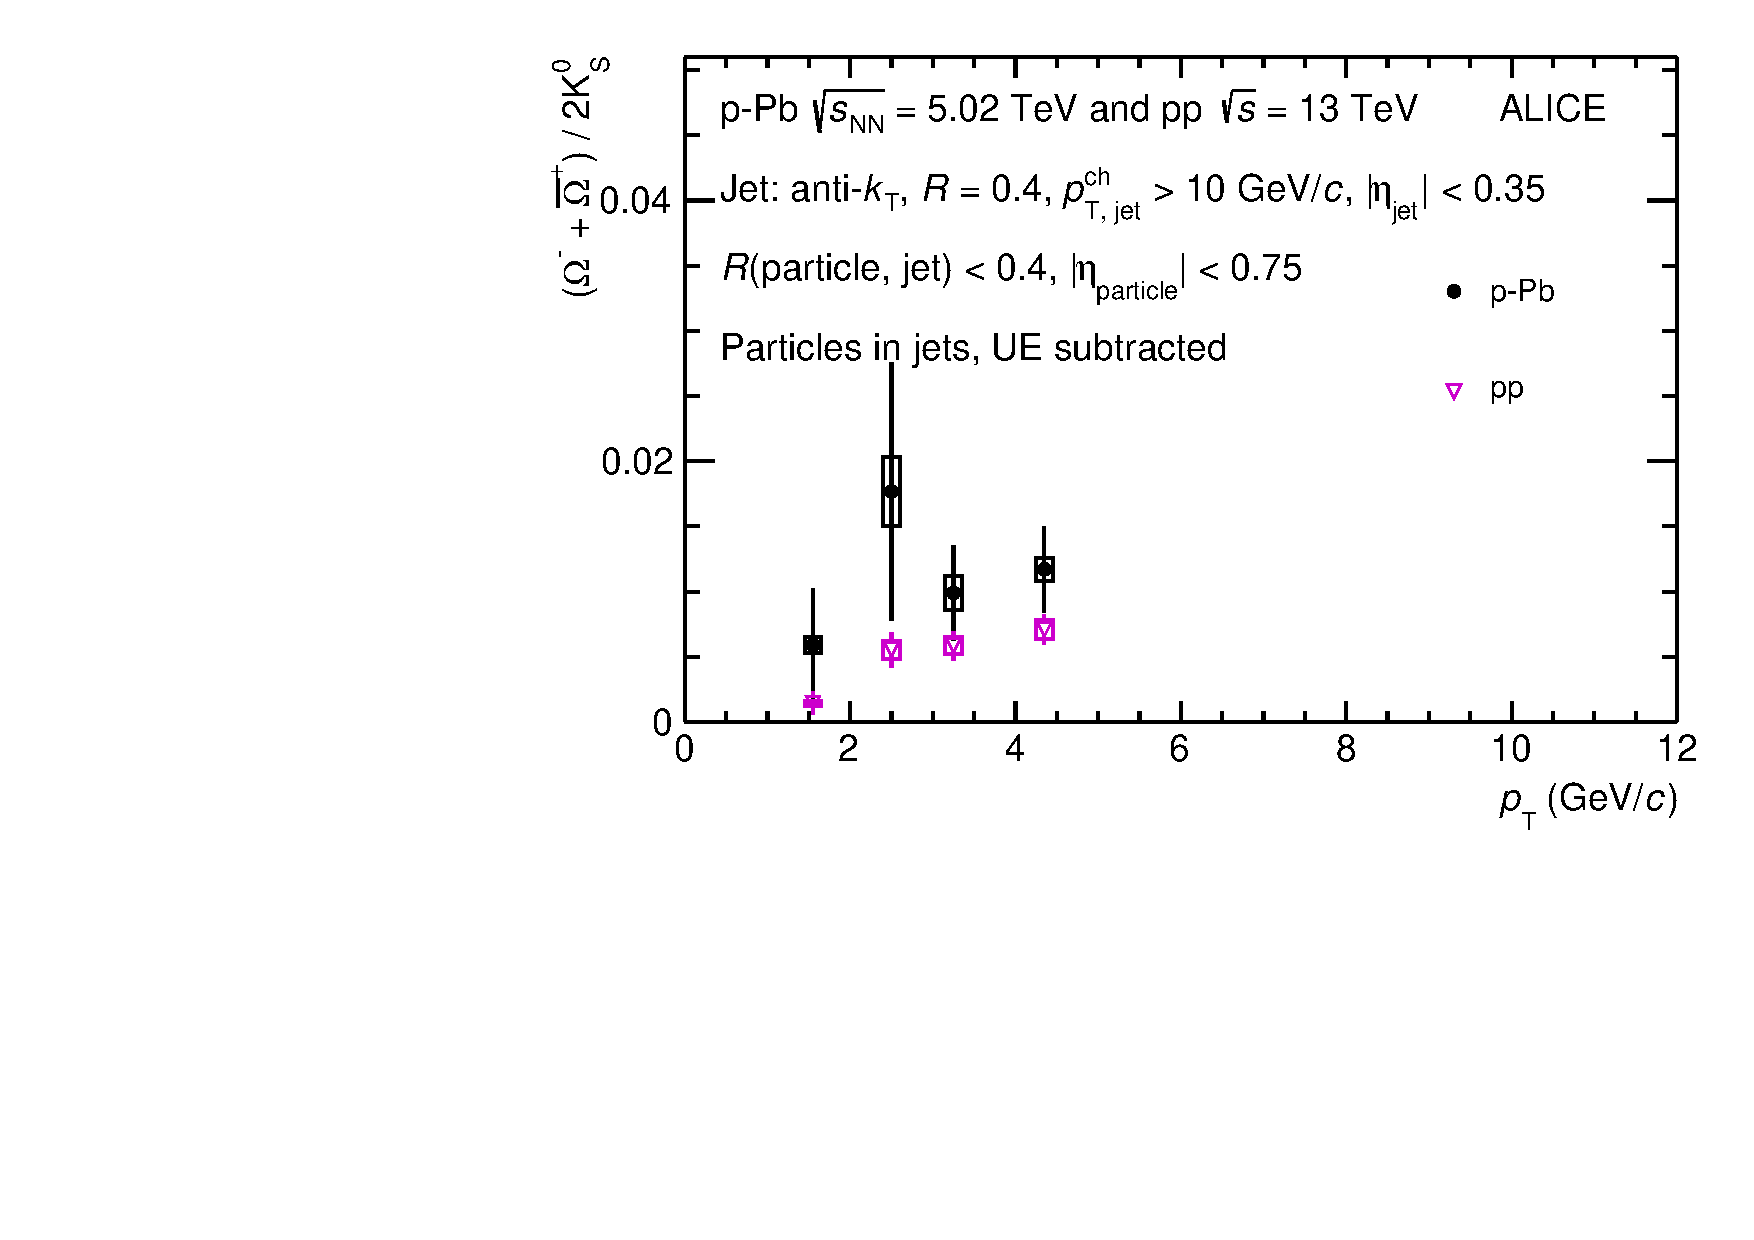
\includegraphics[width=.3\textwidth]{cf09_3}
		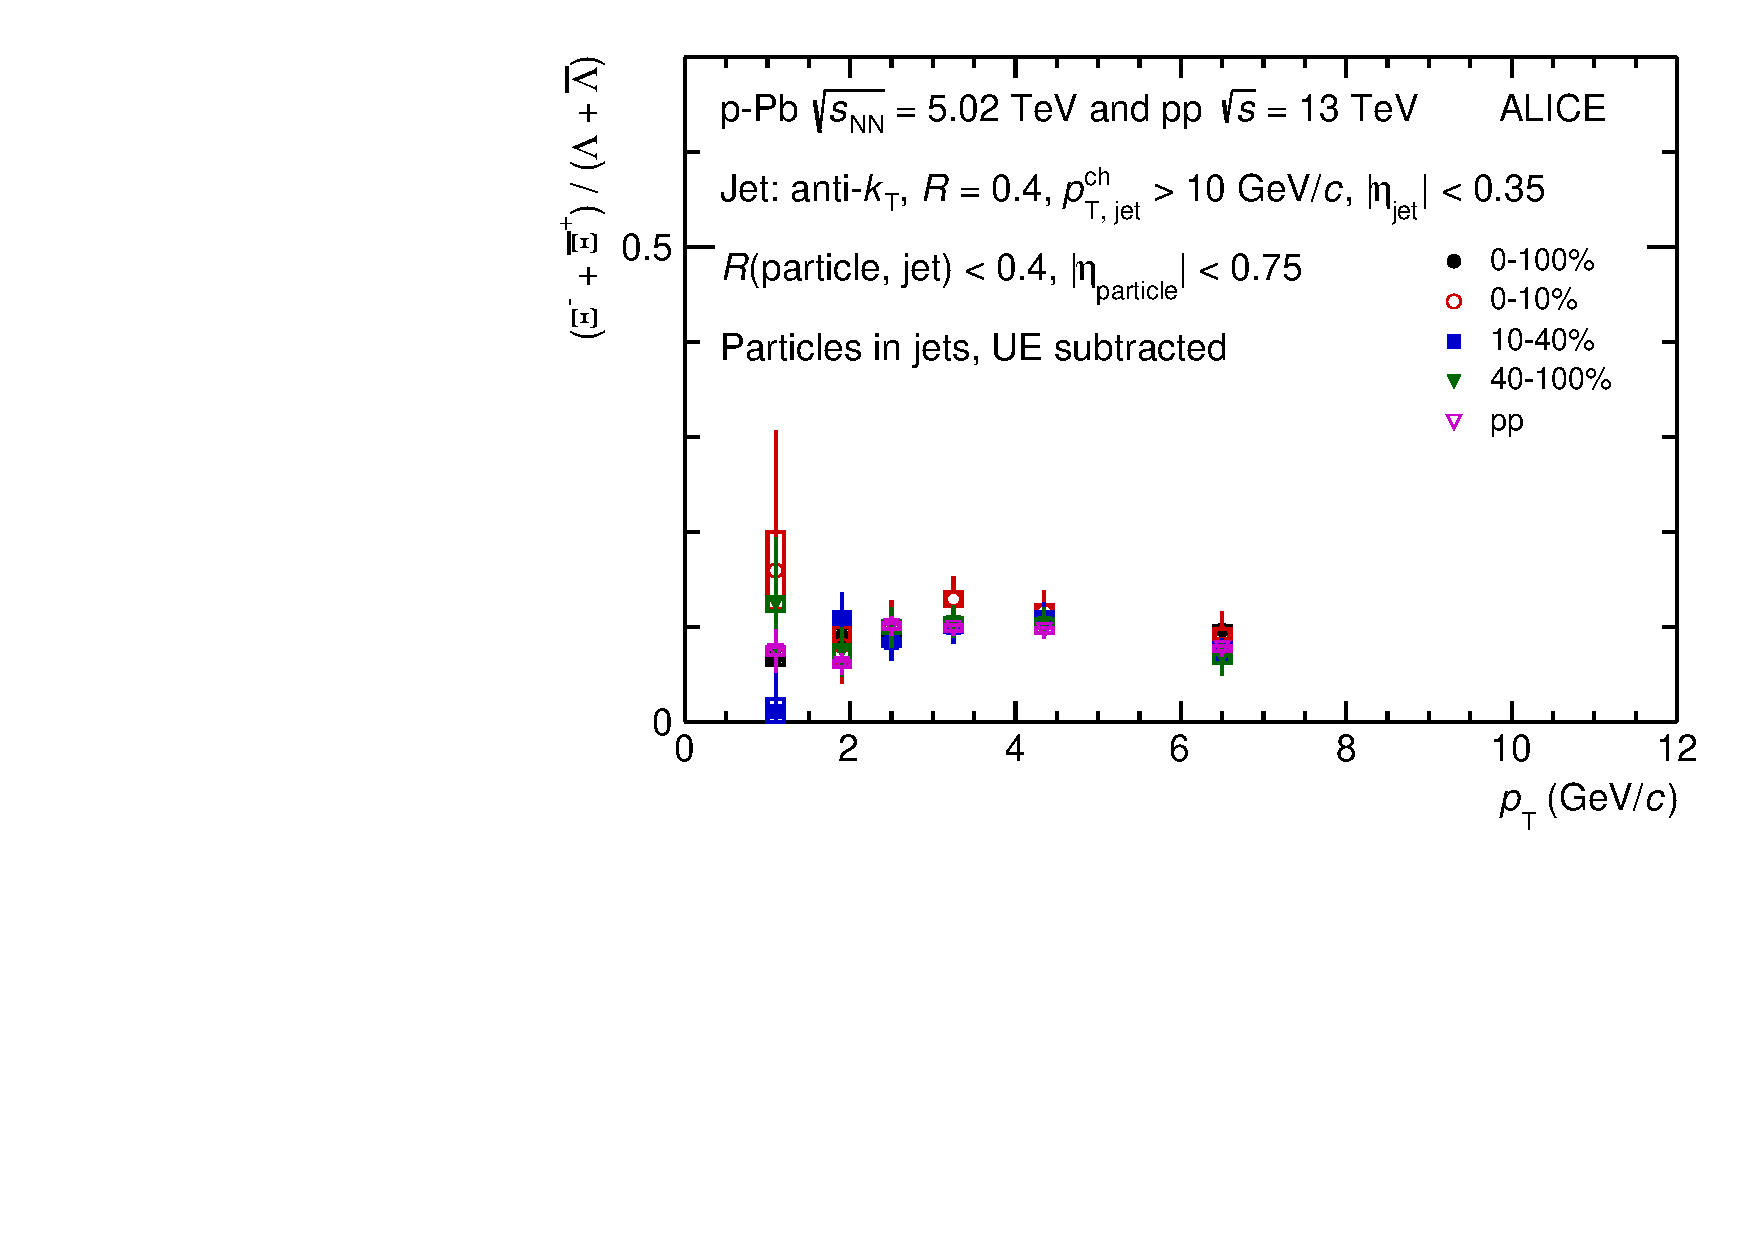
\includegraphics[width=.3\textwidth]{cf09_4}
		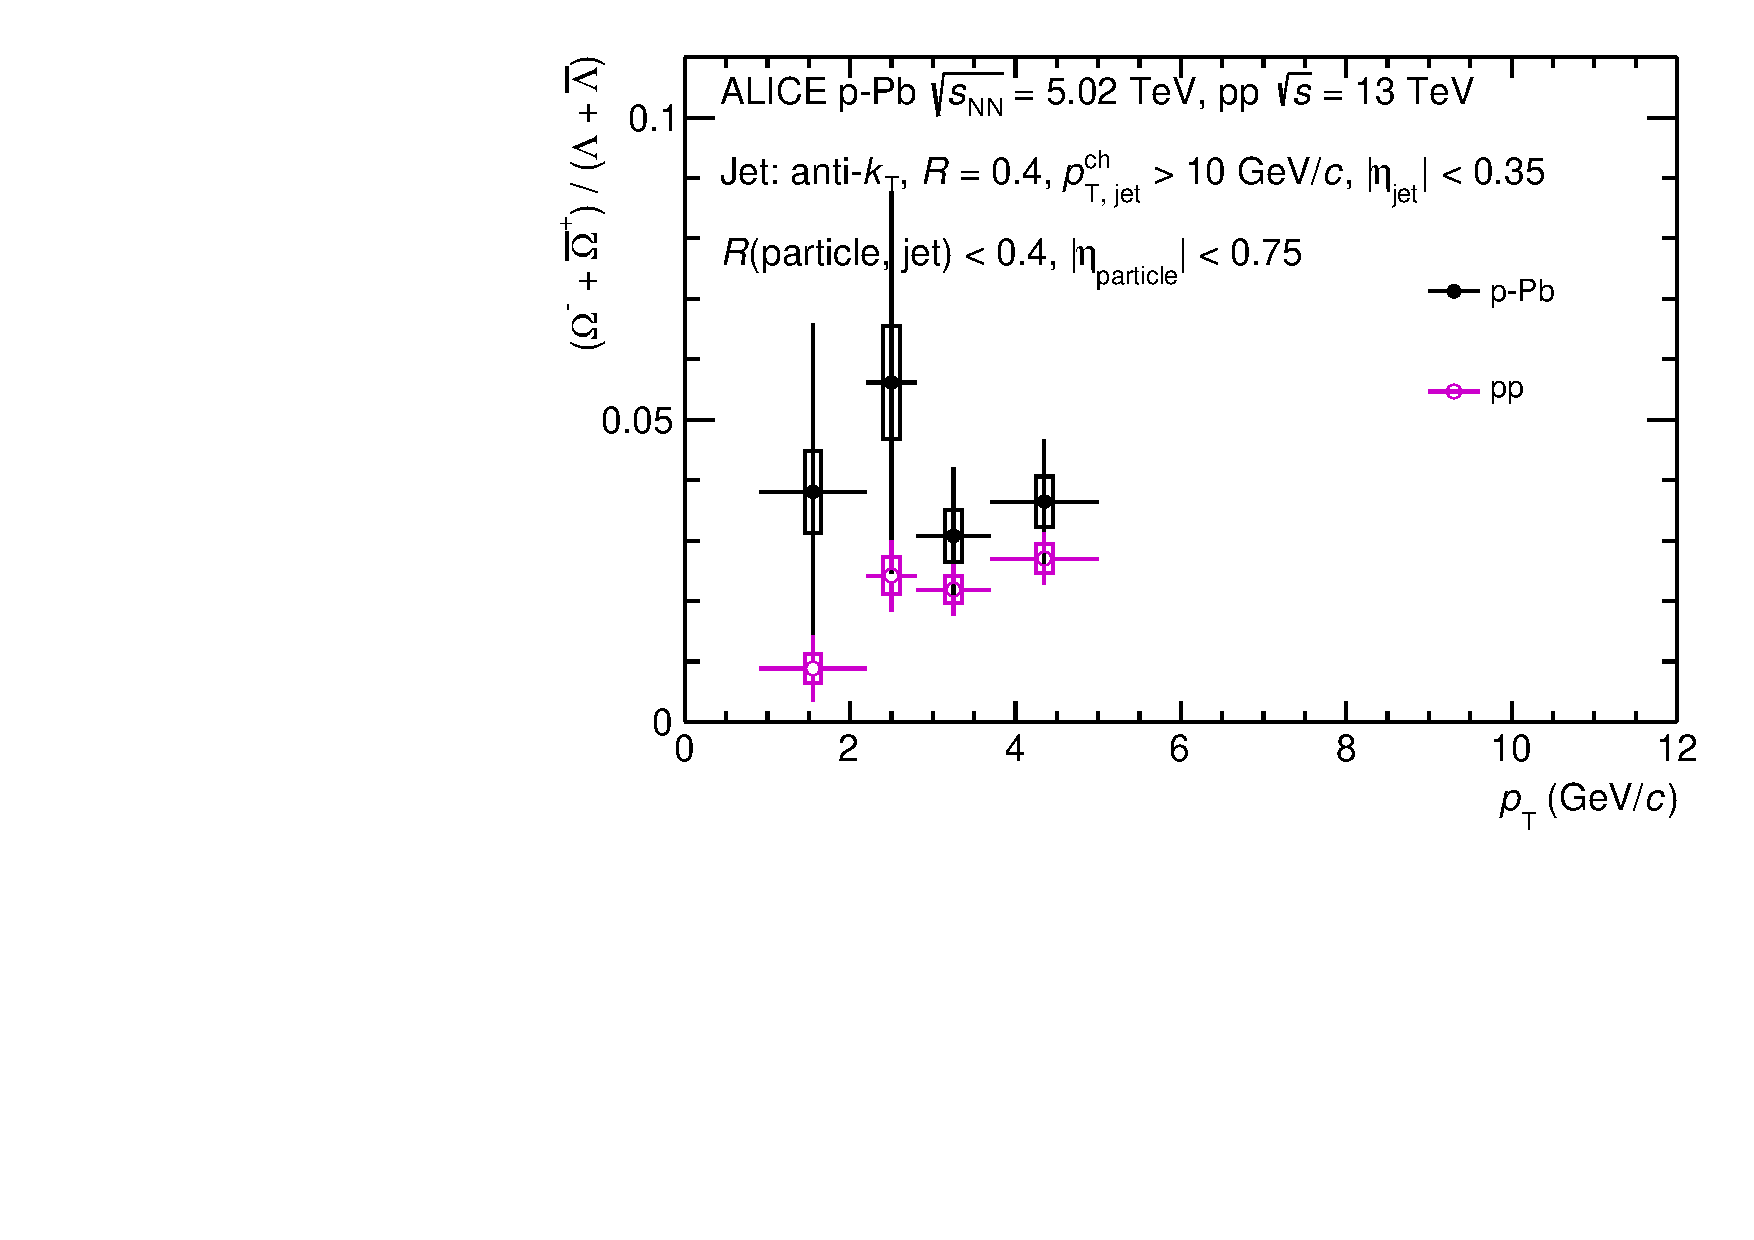
\includegraphics[width=.3\textwidth]{cf09_5}
		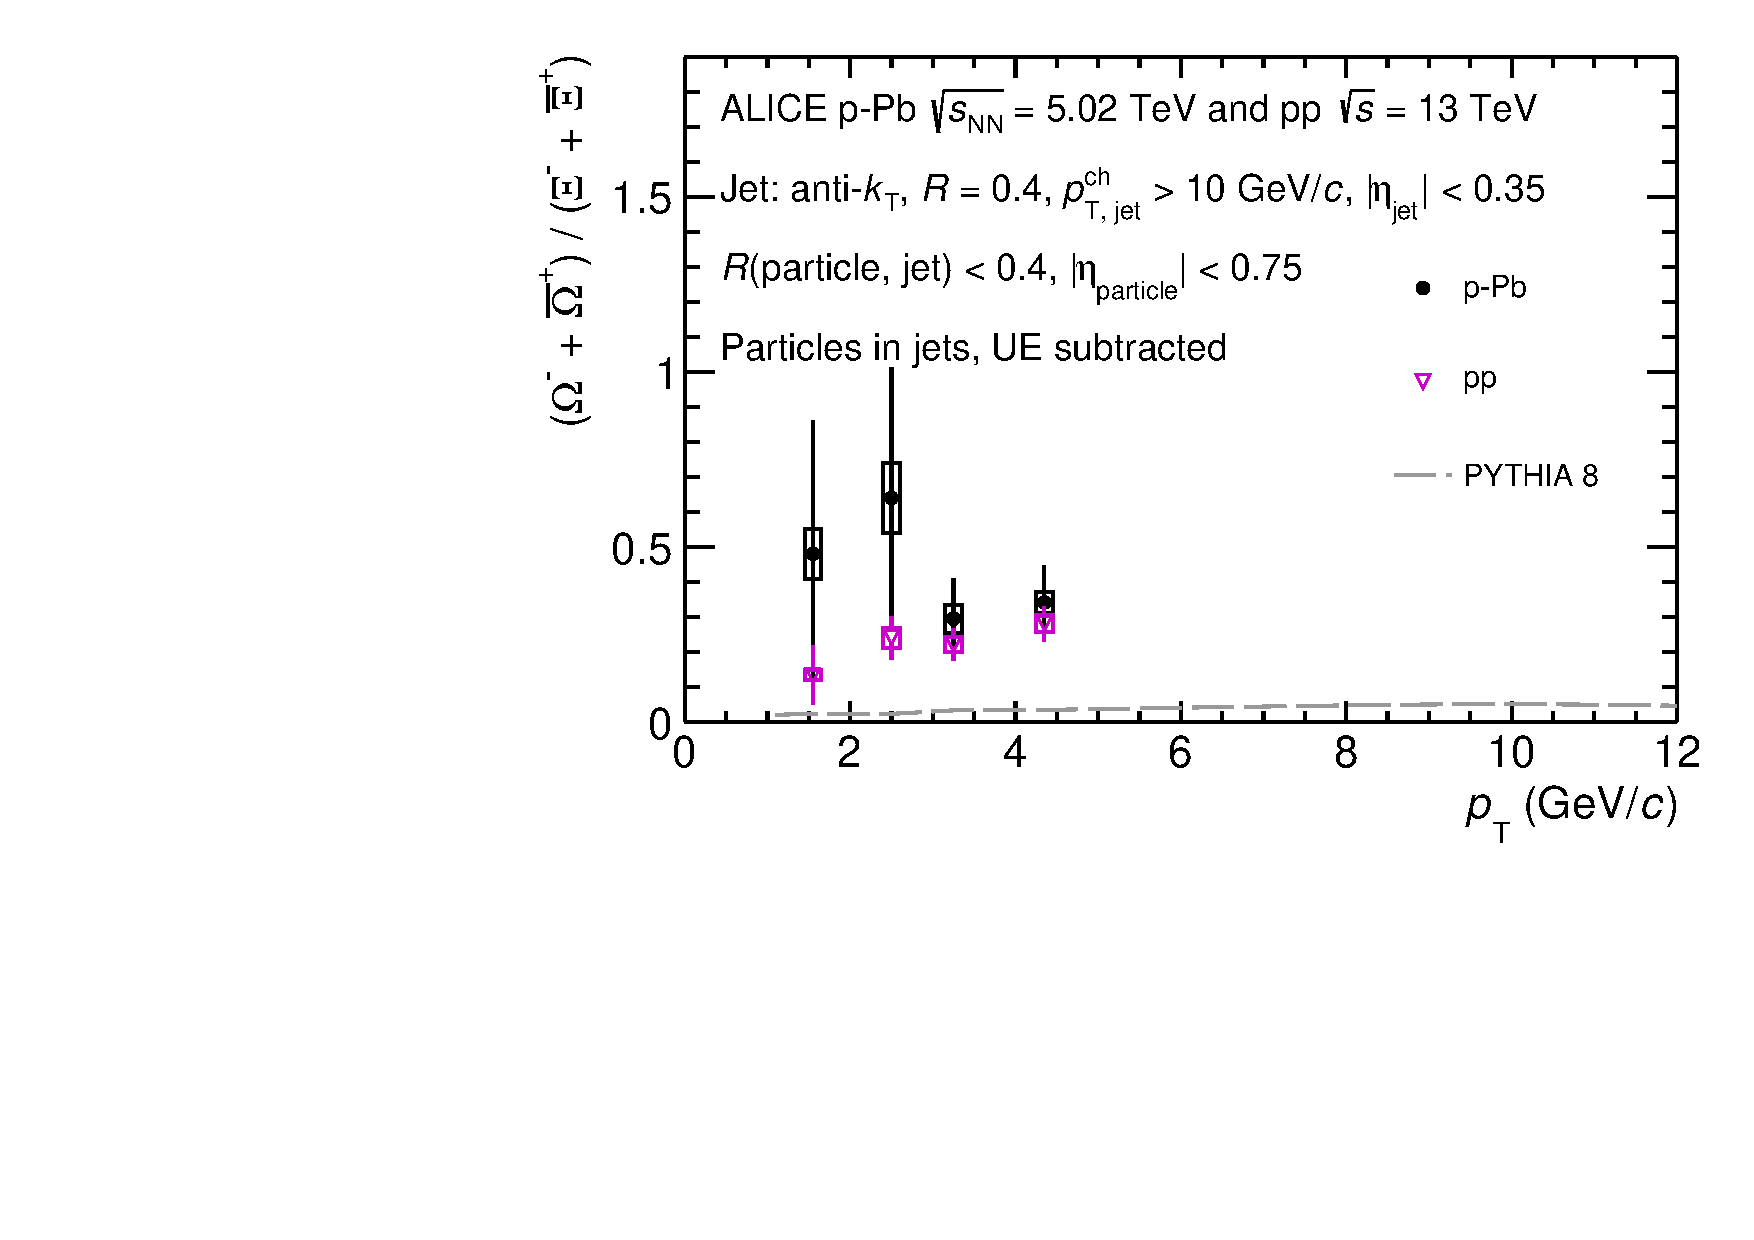
\includegraphics[width=.3\textwidth]{cf09_6}
	\end{center}
	\caption{The baryon-to-meson (top) and baryon-to-baryon(bottom) ratio as a function of particle $\pT$ in jets in \pp (open symbols) and \pPb (full symbols). The different centrality classes for \pPb collisions are depicted with different color.}
	\label{fig:pppPbRatio}
\end{figure}

\subsection{Comparison to models}
\label{subsec:ComToMod}

need to be added.

\begin{figure}[!ht]
	\begin{center}
		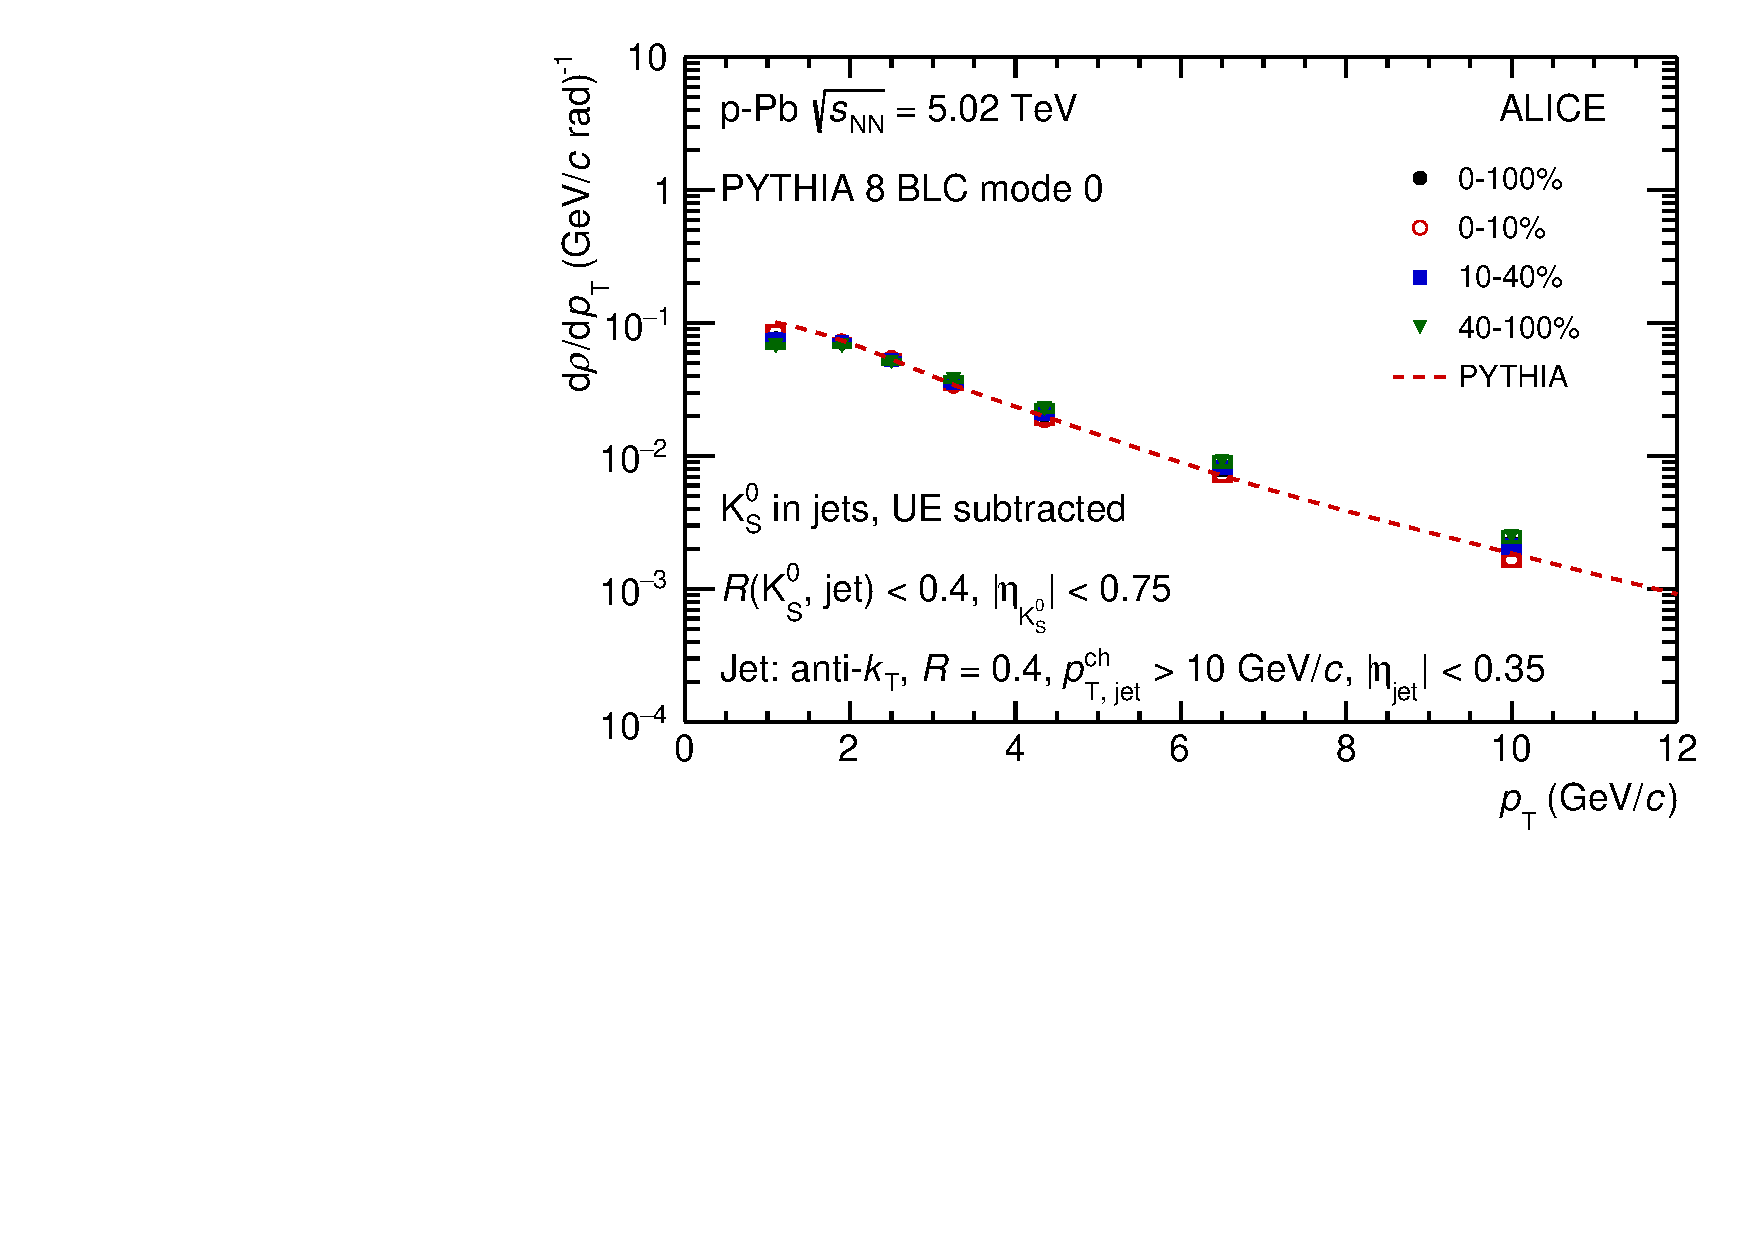
\includegraphics[width=.4\textwidth]{cf10_1}
		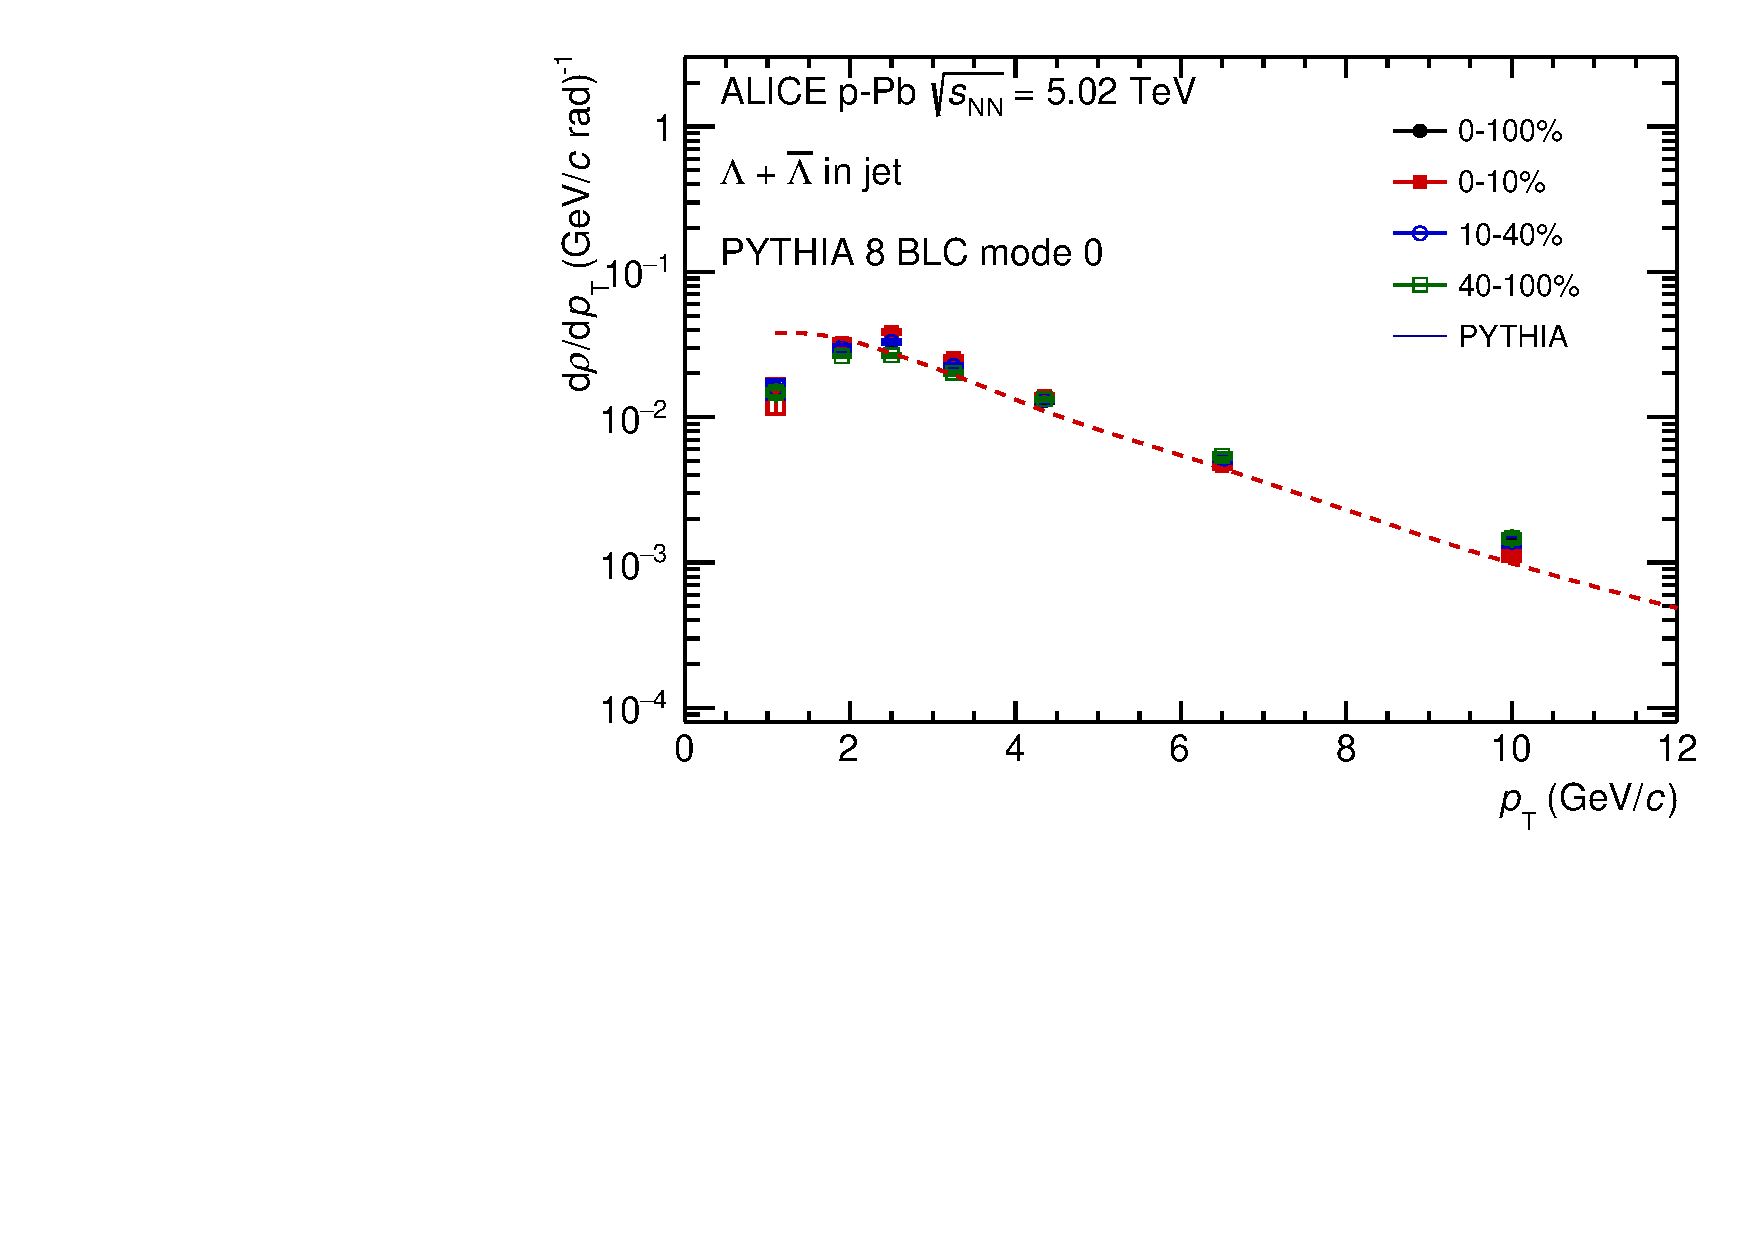
\includegraphics[width=.4\textwidth]{cf10_2}
		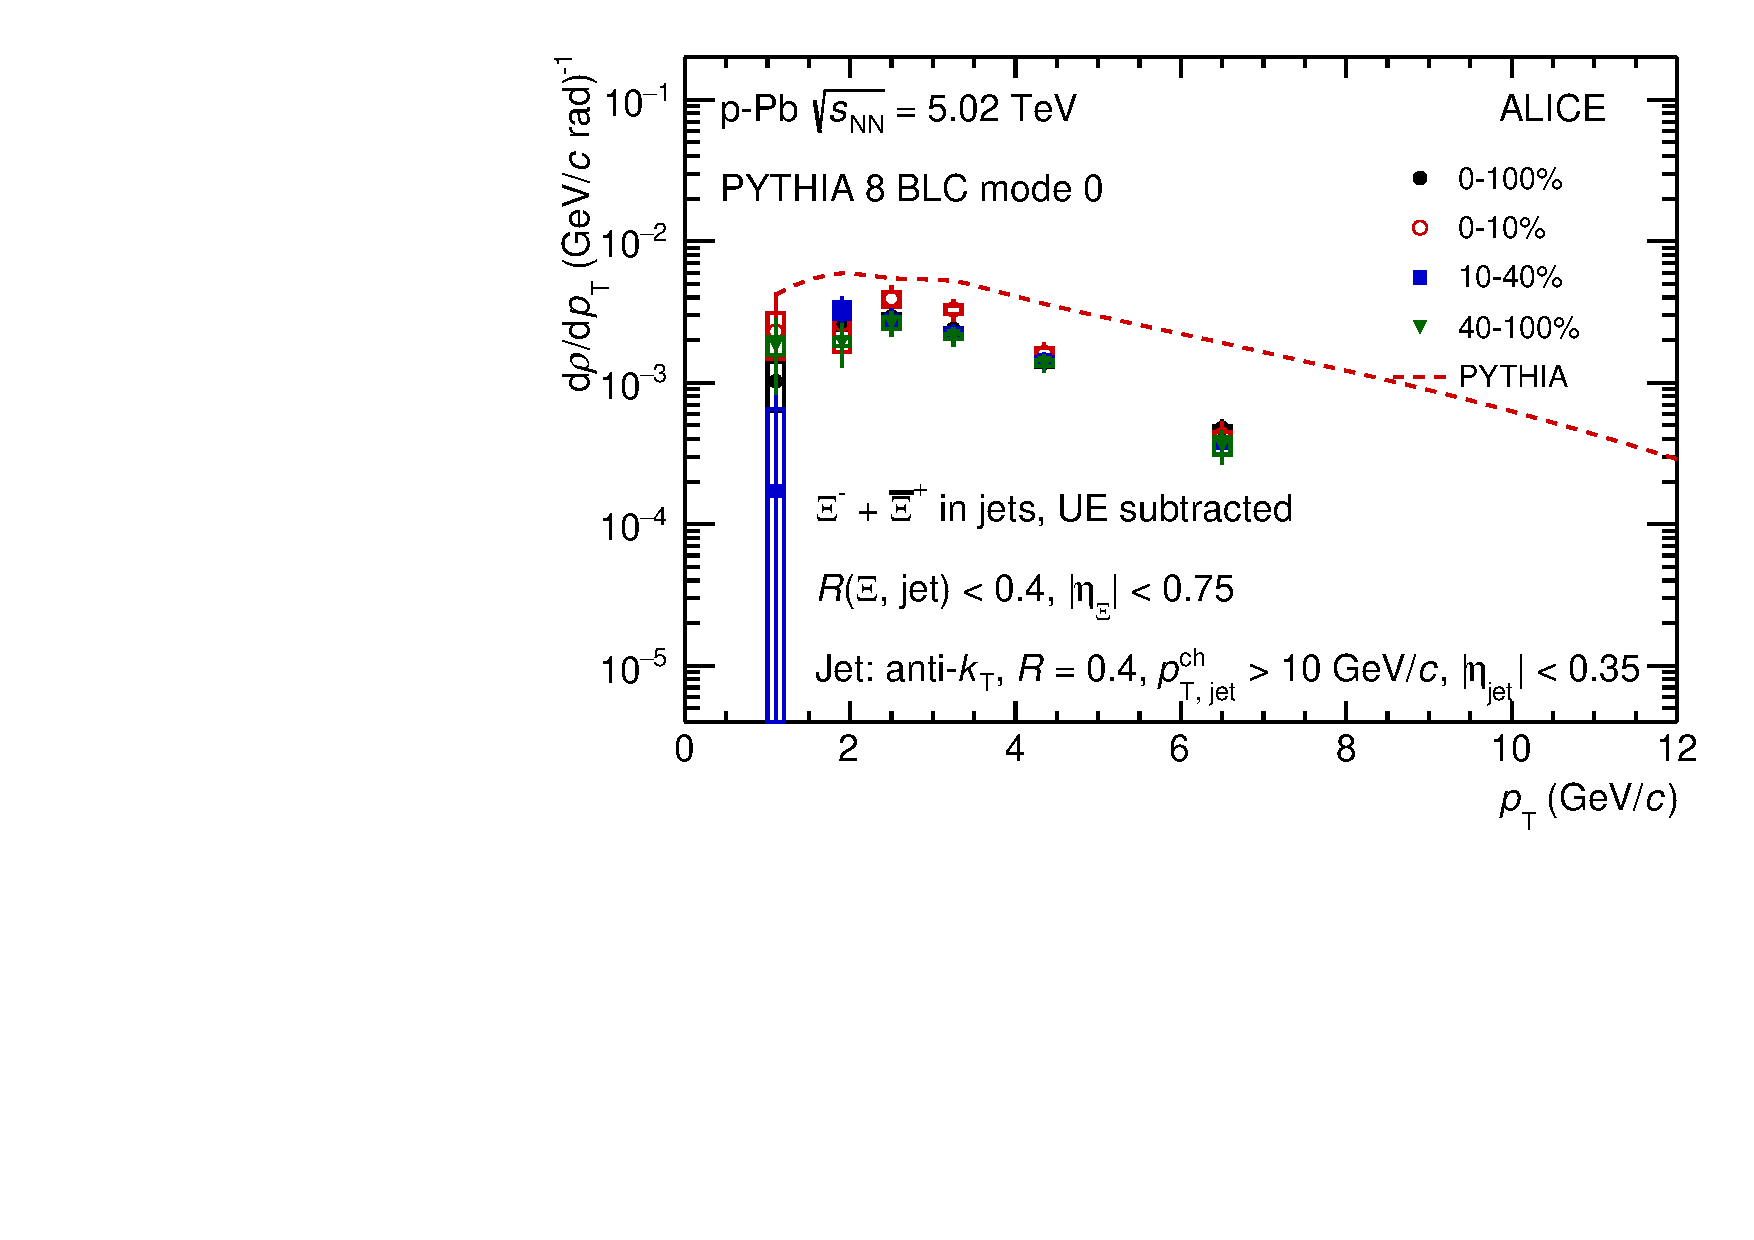
\includegraphics[width=.4\textwidth]{cf10_3}
		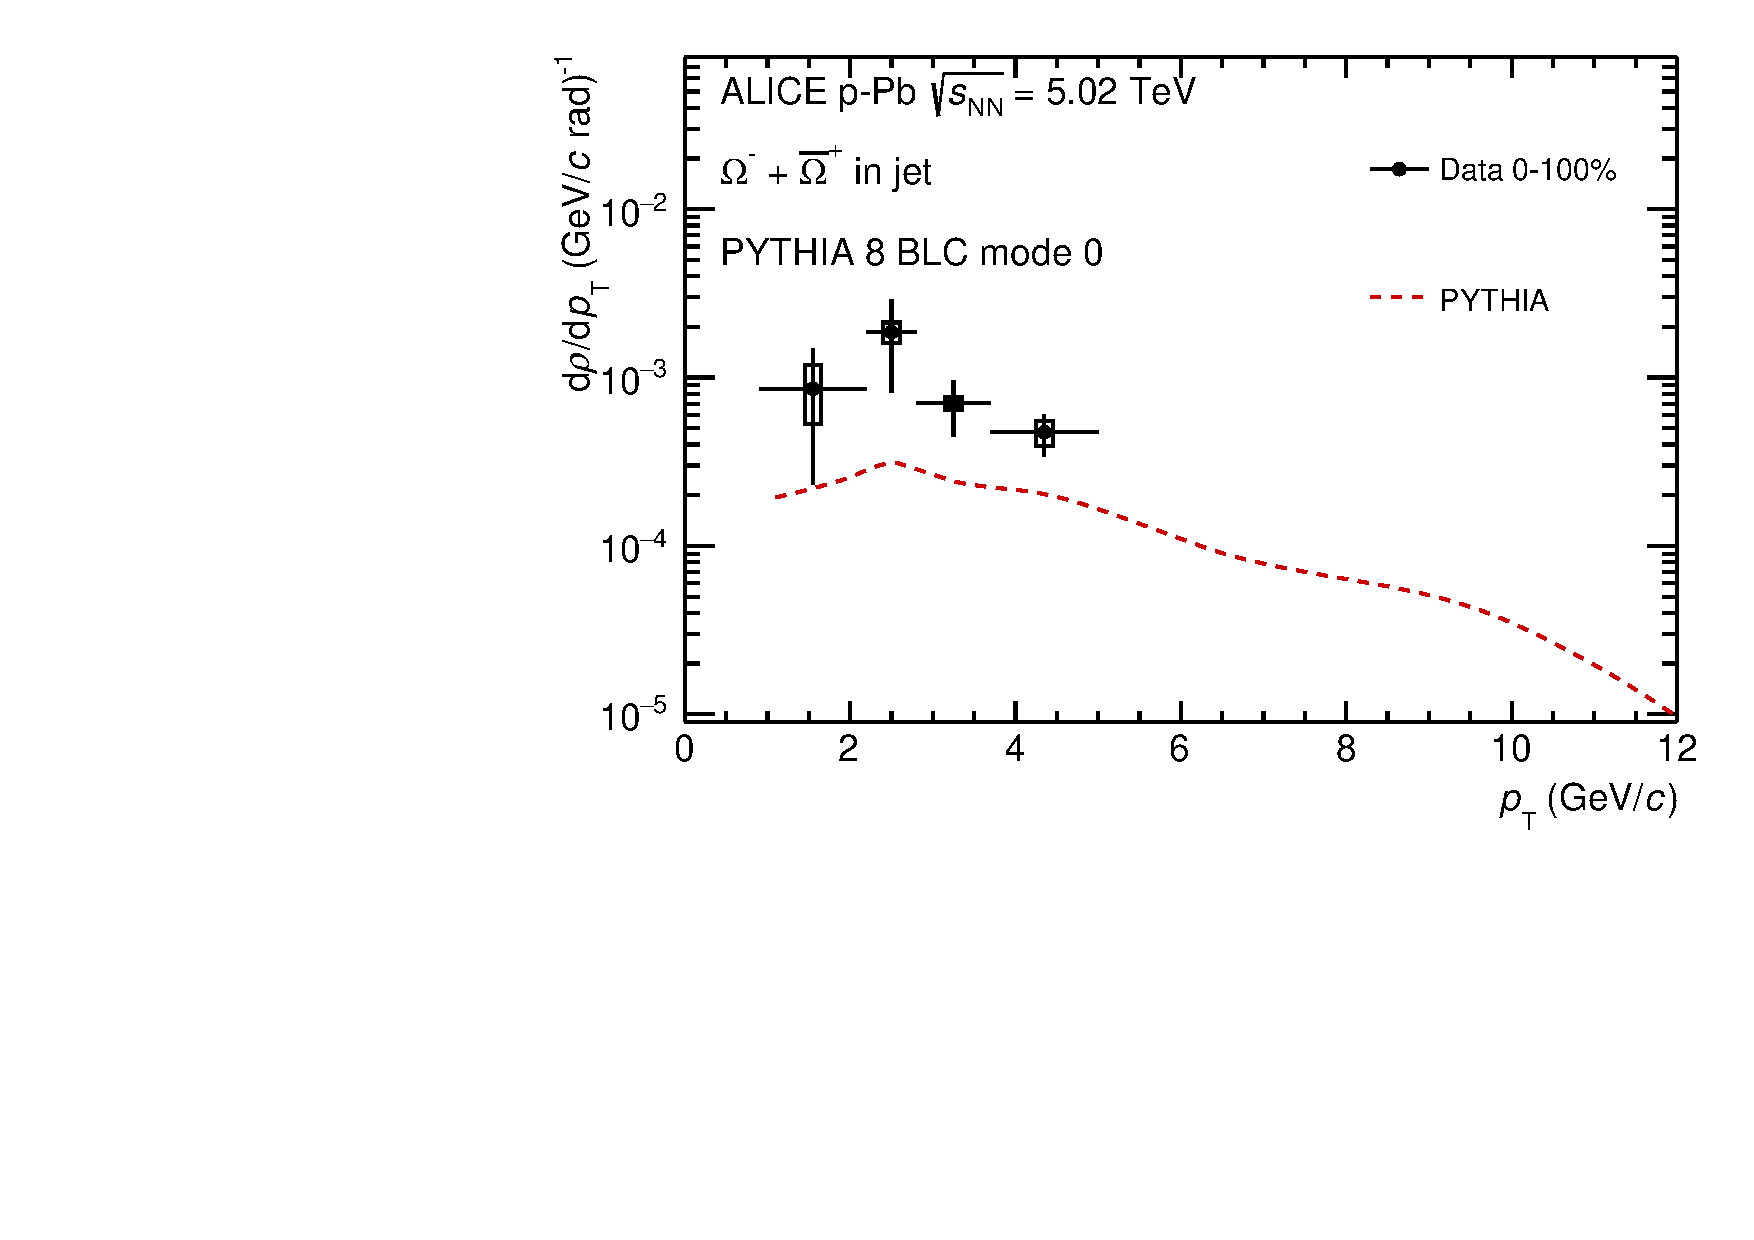
\includegraphics[width=.4\textwidth]{cf10_4}

	\end{center}
	\caption{Particles in jet in \pPb at \fivenn with PYTHIA 8 BLC mode 0}
	\label{fig:pPbpyJESpect}
\end{figure}

